\documentclass[]{fairmeta}

\usepackage{amsmath,amsthm,amssymb,bm}
\usepackage{color}
\usepackage{algorithm}
\usepackage[noend]{algpseudocode}
\usepackage[linesnumbered,ruled,algo2e]{algorithm2e}%
\usepackage{derivative}
\usepackage{longtable}
\usepackage{pifont}
\usepackage{mdframed}
\usepackage{enumitem}
\usepackage{adjustbox}
\usepackage{mathrsfs}

\usepackage[normalem]{ulem}

\usepackage{siunitx}
\usepackage{tocloft}

\let\oldaddcontentsline\addcontentsline
\newcommand{\stoptocentries}{\renewcommand{\addcontentsline}[3]{}}
\newcommand{\starttocentries}{\let\addcontentsline\oldaddcontentsline}

\usepackage{tikz}
\usetikzlibrary{positioning, fit, calc}

\usepackage{booktabs}

% \usepackage{amsmath}
% \usepackage{amssymb}
\usepackage{graphicx}
\usepackage{mathtools}
% \mathtoolsset{showonlyrefs}
\usepackage{amsfonts}
% \usepackage{amsthm,bm}
\usepackage{color}
% \usepackage{enumitem}
\usepackage{dsfont}
% \usepackage{pgfplots}
% \pgfplotsset{width=10cm,compat=1.9}
%  \usepackage{pifont}%http://ctan.org/pkg/pifont
\usepackage{thmtools} 
% \usepackage{thm-restate}
% \usepackage{sidecap}

\declaretheorem[name=Theorem]{thm}
\declaretheorem[name=Proposition]{prop}
\declaretheorem[name=Corollary]{cor}


\newcommand{\cmark}{\ding{51}}%
\newcommand{\xmark}{\ding{55}}%
\newcommand{\R}{\mathbb{R}}
\newcommand{\upmark}{\ding{218}}
\newcommand{\downmark}{\ding{216}}
\newcommand{\norm}[1]{\lVert#1\rVert}
\newcommand{\dotprod}[1]{\langle #1\rangle}
\newcommand{\E}{\mathbb{E}} 
\newcommand{\Et}[1]{\mathbf{E}_t\left[#1\right] } 
\newcommand{\Ev}[1]{\mathbf{E}_v\left[#1\right] } 
\newcommand{\EE}[2]{\mathbf{E}_{#1}\left[#2\right] } 
\newcommand{\Prb}[1]{\mathbf{P}\left[#1\right] }
\newcommand{\Tr}[1]{\mathrm{Tr}( #1)}
\newcommand{\Rea}[1]{\mathrm{Re}[ #1]}
\newcommand{\Ima}[1]{\mathrm{Im}[ #1]}
\newcommand{\eqdef}{\overset{\text{def}}{=}} 
\newcommand{\floor}[1]{\lfloor #1 \rfloor}
\newcommand{\Cov}[1]{\mathrm{Cov}\left[#1\right]}
\newcommand{\Var}[1]{\mathrm{Var}\left[#1\right]}
%\newcommand{\argmin}[1]{\underset{#1}{\text{argmin }}  } 
\newcommand{\breg}[2]{\mathcal{D}_{\Phi}\left(#1,#2\right) }
\newcommand{\xx}{\mathbf{x}}
\newcommand{\yy}{\mathbf{y}}
\newcommand{\zz}{\mathbf{z}}
\newcommand{\hmu}{\hat{\mu}}
\renewcommand{\phi}{\varphi}

%\usepackage{algorithm}
%\usepackage[noend]{algpseudocode}

\newcommand{\carles}[1]{{\color{red}{\bf[Carles:} #1{\bf]}}}
\newcommand{\ricky}[1]{{\color{magenta}{\bf[Ricky:} #1{\bf]}}}
\newcommand{\brian}[1]{{\color{orange}{\bf[Brian:} #1{\bf]}}}

% \newcommand{\carles}[1]{}
% \newcommand{\ricky}[1]{}
% \newcommand{\brian}[1]{}

\setlength{\parskip}{0.5em}
\setlength\parindent{0pt}

\graphicspath {{figures/}}

\newcommand{\N}{\mathbb{N}}
\newcommand{\Ff}{\mathcal{F}}
\newcommand{\Gg}{\mathcal{G}}
\usepackage{hyperref}
\usepackage{caption}
\usepackage[super]{nth}
\delimitershortfall-1sp

\newtheorem{lemma}{Lemma}
\newtheorem{definition}{Definition}
\newtheorem{theorem}{Theorem}
\newtheorem{note}{Note}
\newtheorem{assumption}{Assumption}
\newtheorem{proposition}{Proposition}
\newtheorem{example}{Example}
\newtheorem{remark}{Remark}
\newtheorem{corollary}{Corollary}
\newtheorem{observation}{Observation}
% \newtheorem{algorithm}{Algorithm}
\usepackage{subcaption}
%\newcommand{\corollaryautorefname}{Corollary}

\DeclareMathOperator*{\argmin}{argmin}
\DeclareMathOperator*{\argmax}{argmax}

\DeclarePairedDelimiter\abs{\lvert}{\rvert}

\renewcommand{\sectionautorefname}{Sec.}
\renewcommand{\subsectionautorefname}{Subsec.}
\renewcommand{\appendixautorefname}{App.}
\renewcommand{\theoremautorefname}{Thm.}
\renewcommand{\propositionautorefname}{Prop.}
\renewcommand{\corollaryautorefname}{Cor.}
% \renewcommand(\algorithmautorefname}{Alg.}

\newenvironment{talign*}
 {\let\displaystyle\textstyle\csname align*\endcsname}
 {\endalign}
\newenvironment{talign}
 {\let\displaystyle\textstyle\csname align\endcsname}
 {\endalign}

\makeatletter
\renewcommand{\thealgorithm}{\arabic{algorithm}}
% \@addtoreset{algorithm}{chapter}  % Remove or modify this line if you do not want to reset with chapters
\makeatother

\makeatletter
\DeclareRobustCommand{\cev}[1]{%
  {\mathpalette\do@cev{#1}}%
}
\newcommand{\do@cev}[2]{%
  \vbox{\offinterlineskip
    \sbox\z@{$\m@th#1 x$}%
    \ialign{##\cr
      \hidewidth\reflectbox{$\m@th#1\vec{}\mkern4mu$}\hidewidth\cr
      \noalign{\kern-\ht\z@}
      $\m@th#1#2$\cr
    }%
  }%
}
\makeatother

\definecolor{mygray}{gray}{0.95}
\newcommand{\greybox}[1]{
\vspace{-0.9em}
\begin{center}			% Centering minipage
\vspace{-0.5em}
\colorbox{mygray} {		% Set's the color of minipage
\begin{minipage}{0.987\linewidth} 	% Starts minipage
\centering
\vspace{-0.8em}
{#1}
\end{minipage}}			% End minipage
\end{center}
\vspace{-0.5em}
}

\title{Adjoint Matching: Fine-tuning Diffusion Models as Stochastic Optimal Control}

\author[1]{Carles Domingo-Enrich}
\author[1]{Michal Drozdzal}
\author[1]{Brian Karrer}
\author[1]{Ricky T. Q. Chen}
\affiliation[1]{FAIR, Meta}

\abstract{
    % We perform a detailed analysis of existing and novel training losses for the stochastic optimal control problem, both at the theoretical and the empirical levels. We compare the losses on simple problems where the optimal control can be obtained by other means, and we also run experiments on RL fine-tuning for diffusion models. 
    % Diffusion and flow matching models have achieved state-of-the-art results for generative modeling of continuous data, and they need to be fine-tuned for specialized tasks. In analogy with RLHF for language generation, we formulate diffusion fine-tuning as learning to sample from the tilted distribution $p^*(x) \propto p_{\mathrm{base}}(x) \exp(r(x))$, where $p_{\mathrm{base}}$ is the distribution of the base model and $r$ is a reward model that typically captures sample quality and text-to-sample alignment. We cast this task as a stochastic optimal control (SOC) problem. We proceed to systematically study all the existing and some new deep learning techniques to solve SOC problems, which we benchmark on simple settings. Finally, we compare the performance of the most promising SOC techniques with existing diffusion RL fine-tuning approaches. Some of our algorithms, such as the Adjoint Matching loss, achieve significantly better results, both in terms of average reward $r$ and alternative quality metrics. 
    
    % Diffusion and Flow Matching models are the state-of-the-art generative modeling paradigm of continuous-valued data, but they often need to be fine-tuned for specialized tasks. 
    % In particular, Reinforcement Learning from Human Feedback (RLHF) aims to align diffusion models with human preferences, formulated as learning to sample from the fine-tuned distribution $p^*(x) \propto p^{\mathrm{base}}(x) \exp(r(x))$, where $p^{\mathrm{base}}$ is the distribution of a pretrained diffusion model and $r$ is a reward model that typically captures sample quality and text-to-image alignment. 
    
    % In this work, we cast fine-tuning diffusion models as a stochastic optimal control (SOC) problem, and find that the na\"ive formulation will theoretically introduce bias, an issue that prior works have struggled with. To address this, we propose an extremely simple solution: by choosing a particular noise schedule, we arrive at an SOC formulation where the solution is the desired distribution.

    % We next address the problem of choosing an SOC algorithm. In light of the success of diffusion models and Flow Matching, we propose a novel matching objective called Adjoint Matching, an entirely new approach in the taxonomy of SOC algorithms. 
    % In particular, it is faster to compute than the continuous adjoint method, it is more scalable than importance-weighted objectives, and it performs favorably on both synthetic SOC problems and large scale diffusion model fine-tuning. 
    % Ultimately, we find our approach can significantly improve diffusion fine-tuning, outperforming existing methods on the training reward function and achieving better generalization to other human preference reward models, while retaining the sample diversity of the original model.
    % \ricky{suggestion from Michal: add diversity metric into evaluation}

    Diffusion and Flow Matching models are the state-of-the-art generative modeling paradigm for continuous-valued data. Reinforcement Learning from Human Feedback (RLHF) aims to align such models with human preferences, by learning to sample from the fine-tuned distribution $p^*(x) \propto p^{\mathrm{base}}(x) \exp(r(x))$, where $p^{\mathrm{base}}$ is the distribution of a pretrained model and $r$ is a reward model that captures sample quality and text-to-image alignment. 
    
    In this work, we cast fine-tuning diffusion models as stochastic optimal control (SOC): we introduce an SOC problem such that its solution allows us to sample from the fine-tuned distribution $p^*$. Critically, our SOC problem uses a specific fine-tuning noise schedule, independent of the noise schedule that one wishes to use at inference. To solve this SOC problem, we propose a new algorithm named Adjoint Matching which outperforms all existing SOC algorithms in realistic settings: it is faster to compute and more precise than other adjoint-based methods, and more scalable than importance-weighted objectives. To support this claim, we provide a detailed taxonomy of algorithms to solve SOC problems, including five novel ones, and we benchmark them on synthetic settings.

    We find that our approach significantly improves diffusion fine-tuning, achieving higher values for the training reward model and better generalization to other human preference reward models, while retaining the sample diversity of the original diffusion model.
}

\stoptocentries

% \date{\today}
\correspondence{Carles Domingo-Enrich at \email{cd2754@nyu.edu}}

\metadata[Code]{\url{TBD}}

\begin{document}

\maketitle

\section{Introduction}
\label{sec:intro}

Diffusion models %(\textcolor{red}{cite} Sohl-Dickstein et al., 2015; Song \& Ermon, 2019; Ho et al., 2020; Song et al., 2021b; Kingma et al., 2021)
\citep{song2019generative,ho2020denoising,song2021scorebased,kingma2021ondensity}
and flow matching models \citep{lipman2022flow,albergo2022building} have achieved state-of-the-art generative modeling performance for all kinds of continuous data, including text-to-image, text-to-video, and text-to-audio. For most use cases, the base model does not achieve the desired behavior or sample quality due to subpar pretraining data, distribution shifts, or small model capacity. To obtain better performance in specialized tasks, it is common to resort to techniques such as classifier and classifier-free guidance \citep{dhariwal2021diffusion,ho2021classifierfree} or noise sample optimization \citep{wallace2023endtoend,benhamu2024dflow} in order to get better text-to-sample alignment, or to fine-tune on curated datasets such as LAION Aesthetics \citep{schuhmann2022laion} to improve sample quality.

In the adjacent field of large language models (LLMs), the behavior of the model is aligned to user preferences through fine-tuning with reinforcement learning (RL), which has given rise to RL from human feedback (RLHF).  
% Ziegler et al. 2019; Stiennon et al. 2020; Ouyang et al. 2022; Bai et al. 2022a). 
Either explicitly or implicitly, RLHF deals with a reward model $r$ that captures human preferences. Their goal is to modify the model such that it generates the following distribution: 
% \begin{talign} \label{eq:p_star_info}
% p^*(x) = \frac{p_{\mathrm{base}}(x) \exp(r(x))}{\int p_{\mathrm{base}}(y) \exp(r(y)) dy}, 
% \end{talign}
\begin{talign} \label{eq:p_star_info}
p^*(x) \propto p^{\mathrm{base}}(x) \exp(r(x)),
\end{talign}
where $p_{\mathrm{base}}$ is the base model distribution. There are two main RLHF strategies \textit{reward-based} approach \citep{ziegler2020finetuning,stiennon2020learning,ouyang2022training,bai2022training} and \textit{direct preference optimization} (DPO; \cite{rafailov2023direct}).
The \textit{reward-based} approach \citep{ziegler2020finetuning,stiennon2020learning,ouyang2022training,bai2022training} consists in learning the reward model $r(x)$ from human preference data (typically human choices between pairs of generations for the same prompt), and then solving a maximum entropy RL problem with rewards produced by $r$, using e.g. proximal policy optimization (PPO; \cite{schulman2017proximal}). DPO merges the two previous steps into one: there is no need to learn $r$ as human preference data is directly used to fine-tune the model. However, DPO has narrower applicability as it cannot handle generic rewards, and is not well suited for highly complex tasks. %\textcolor{red}{What is the downside of DPO?}

Inspired by RLHF, %supervised and 
reinforcement learning methods have been developed to fine-tune diffusion models on human preference data; either using a reward-based approach \citep{fan2023optimizing,black2024training,fan2023dpok,xu2023imagereward,clark2024directly,uehara2024finetuning,uehara2024understanding},
or direct preference optimization \citep{wallace2023diffusion}. Reward models such as PickScore \citep{kirstain2023pickapic}, Human Preference Score v2 \citep{wu2023humanpreferencescorev2}, and ImageReward \citep{xu2023imagereward}, which are trained on human judgements between pairs of images generated by diffusion models for the same prompt, capture a combination of image quality and text-to-image alignment.

The main contributions of our paper are as follows:
\begin{enumerate}[label=(\roman*)]
    \item Through the connection between maximum entropy RL and stochastic optimal control (SOC) (\autoref{subsec:max_ent_RL}), in \autoref{subsec:diffusion_SOC} we present the
    % stochastic optimal control
    SOC problem that needs to be solved to fine-tune a diffusion model (DDPM, DDIM) or a flow matching model such that it generates the tilted distribution $p^*$ \eqref{eq:p_star_info}. Interestingly, the base dynamics for the SOC problem may differ from the dynamics that one intends to use at inference time; e.g., even if we want to use DDIM in practice, we need to fine-tune using DDPM.
    \item Since diffusion fine-tuning amounts to solving SOC problems, we review existing deep learning loss functions to tackle such problems (\autoref{subsec:existing_losses}), and we propose additional ones, among them the Adjoint Matching loss.
    % four additional algorithms (\autoref{sec:new_losses}): the Work Adjoint, Work-SOCM, Cost-SOCM and Unweighted SOCM losses. 
    We organize all 
    % the existing algorithms 
    the loss functions
    into a taxonomy (\autoref{fig:SOC_taxonomy}), identifying those losses that have equal gradients in expectation. In \autoref{sec:simple_exp} we benchmark all of them on four simple SOC problems for which the optimal control is known, such that we can measure the control $L^2$ error incurred by each one. 
    % In these simple settings, the best-performing algorithms are those based on the stochastic optimal control matching (SOCM) framework \citep{domingoenrich2023stochastic}, followed by algorithms based on the adjoint method.
    \item Finally, in \autoref{sec:diff_finetuning_exp} we conduct fine-tuning experiments on a text-to-image flow matching model. We benchmark the most promising SOC algorithms introduced in previous sections against the existing reward-based %diffusion fine-tuning 
    approaches in the literature. Our experiments showcase that several SOC algorithms, and in particular the Adjoint Matching loss, outperform all existing methods in terms of the average reward obtained, and when measuring sample quality using alternative metrics (\textcolor{red}{check}).
\end{enumerate}

\section{Related work} 
Among existing reward-based diffusion fine-tuning methods, \cite{fan2023optimizing} interpret the denoising process as a multi-step decision-making task and use policy gradient algorithms to fine-tune diffusion samplers. They restrict their attention to rewards that are integral probability metrics between a target distribution and the generated distribution. \cite{black2024training,fan2023dpok} extend policy gradient fine-tuning to arbitrary reward functions; \cite{black2024training} also consider KL-regularized rewards (see \autoref{subsec:max_ent_RL}) but do not make the subtle yet critical connection to the tilted distribution $p^*$ \eqref{eq:p_star_info} that we flesh out in \autoref{subsec:diffusion_SOC}. 
These approaches based on policy gradients to not take advantage of the differentiability of the reward model $r$, which is a key feature that does not play a role in classical RL but dramatically improves fine-tuning performance. The fine-tuning algorithms of \cite{xu2023imagereward,clark2024directly} do take gradients of the reward model, but their behavior is not well understood and unrelated to the tilted distribution $p^*$: \cite{xu2023imagereward} takes gradients of the reward applied on the denoised sample at different points in time, and \cite{clark2024directly} backpropagates the reward function through all or part of the diffusion trajectory. Finally, \cite{uehara2024finetuning} also fine-tune diffusion models with the goal of sampling from the tilted distribution \eqref{eq:p_star_info}, but their approach is much more involved than ours as it requires learning a value function, and solving two stochastic optimal control problems.

% \textcolor{red}{Add additional related work (find citations for alternative methods)}

\section{Background: diffusion models and flow matching} \label{sec:background}

Diffusion models and Flow Matching are generative modeling techniques that can be understood from the perspective of stochastic interpolants. Given random variables $\bar{X}_0 \sim N(0,I)$ and $\bar{X}_1$ sampled from the training data, the stochastic interpolant $\bar{\bm{X}} = (\bar{X}_t)_{t \in [0,1]}$ is defined as 
\begin{talign} \label{eq:stochastic_interpolant}
\bar{X}_t = \beta_t \bar{X}_0 + \alpha_t \bar{X}_1,
\end{talign}
where $(\alpha_t)_{t \in [0,1]}, (\beta_t)_{t \in [0,1]}$ are increasing and decreasing functions such that $\alpha_0 = \beta_1 = 0$ and $\alpha_1 = \beta_0 = 1$. Diffusion models and Flow Matching construct stochastic or ordinary differential equations (SDEs/ODEs) such that their solution $\bm{X} = (X_t)_{t \in [0,1]}$ has the same time marginals as the stochastic interpolant $\bar{\bm{X}}$, i.e. such that the distributions of $X_t$ and $\bar{X}_t$ are equal for all times. Since $\bar{X}_1$ has the same distribution as the training data, solving such \textit{inference SDEs} is a way to generate artificial samples.

\subsection{Diffusion models: DDIM and DDPM} \label{subsec:background_diffusion}
% Diffusion models are based on pairs of forward and backward stochastic differential equations. The forward process starts from the data distribution $p_1$ that one wants to model, and ends at a distribution $p_0$ which is easy to sample from, typically a standard Gaussian. The backward process, which is the one that is simulated at inference time, starts from the distribution $p_0$ and ends at the distribution $p_1$. 
Denoising Diffusion Implicit Models (DDIM; \cite{song2022denoising}), and Denoising Diffusion Probabilistic Models (DDPM; \cite{ho2020denoising}), which are a particular case of the former, are the most commonly used diffusion models for image, audio, and video applications. The DDIM inference update \citep[Eq.~12]{song2022denoising} is\footnote{We 
% keep 
depart from the notation in \cite{song2022denoising} 
% up to a flip in 
by flipping
the direction of time, for ease of presentation, and using $\gamma_k$ instead of $\alpha_k$.}
\begin{talign} \label{eq:DDIM_original_main}
    % x_{k+1} = \sqrt{\alpha_{k+1}}
    % \big( \frac{x_{k} - \sqrt{1-\alpha_k} \epsilon(x_k,k)}{\sqrt{\alpha_k}} \big)
    % + \sqrt{1-\alpha_{k+1} - \sigma_{k}^2} \epsilon(x_k,k) +
    % \sigma_{k} \varepsilon_{k},
    % \qquad \varepsilon_k \sim N(0,I), \ x_0 \sim N(0,I),
    x_{k+1} = \sqrt{\gamma_{k+1}}
    \big( \frac{x_{k} - \sqrt{1-\gamma_k} \epsilon(x_k,k)}{\sqrt{\gamma_k}} \big)
    + \sqrt{1-\gamma_{k+1} - \sigma_{k}^2} \epsilon(x_k,k) +
    \sigma_{k} \varepsilon_{k},
    \qquad \varepsilon_k \sim N(0,I), \ x_0 \sim N(0,I),
\end{talign}
where $\gamma_k$ is an increasing sequence such that $\gamma_0 = 0$, $\gamma_K = 1$, and the sequence $\sigma_k$, known as the noise schedule, is arbitrary.
That is, one samples an initial Gaussian random variable $x_0$, and applies the stochastic update \eqref{eq:DDIM_original_main} iteratively $K$ times in order to obtain an artificial sample $x_K$. Updates can be interpreted as progressively denoising the iterate: $x_0$ is completely noisy and $x_K$ is fully denoised. The map $\epsilon(x_k,k)$, which is a neural network, is trained to predict the noise of $x_k$. When the noise schedule is $\sigma_k = \sqrt{
% \frac{1-\alpha_{k+1}}{1-\alpha_k}\big(
% 1 - \frac{\alpha_k}{\alpha_{k+1}}
1 - \frac{\gamma_k}{\gamma_{k+1}}
% \big)
}$, DDIM reduces to DDPM\footnote{Up to first order approximations.}, which appeared first:
\begin{talign} \label{eq:DDPM_discrete}
    % x_{k+1} = \sqrt{\frac{\alpha_{k+1}}{\alpha_{k}}} x_k - \big( 1-\frac{\alpha_k}{\alpha_{k+1}} \big) \frac{\epsilon(x_k,k)}{\sqrt{1-\alpha_{k+1}}} + \sqrt{1-\frac{\alpha_k}{\alpha_{k+1}}} \epsilon_k,
    % \qquad \epsilon_k \sim N(0,I), \ x_0 \sim N(0,I),
     x_{k+1} = \sqrt{\frac{\gamma_{k+1}}{\gamma_{k}}} x_k - \big( 1-\frac{\gamma_k}{\gamma_{k+1}} \big) \frac{\epsilon(x_k,k)}{\sqrt{1-\gamma_{k+1}}} + \sqrt{1-\frac{\gamma_k}{\gamma_{k+1}}} \epsilon_k,
    \qquad \epsilon_k \sim N(0,I), \ x_0 \sim N(0,I).
\end{talign}
Up to first-order approximations, the DDIM update \eqref{eq:DDIM_original_main} and the DDPM update \eqref{eq:DDPM_discrete}
% can be written in a simpler form (see \autoref{subsec:continuous_DDIM}): \textcolor{red}{remove this, all explanation in appendix}
% \begin{talign} \label{eq:DDIM_approx_main}
%     x_{k+1} = \big( 1 + \frac{\alpha_{k+1} - \alpha_k}{2\alpha_k} \big) x_k - \big( \frac{\alpha_{k+1} - \alpha_k}{2\alpha_k} + \frac{\sigma_{k}^2}{2} \big) \frac{\epsilon(x_k,k)}{\sqrt{1-\alpha_{k+1}}} + \sigma_k \epsilon_k, \qquad x_0 \sim N(0,I).
% \end{talign}
% And equation \eqref{eq:DDIM_approx_main} 
can be interpreted as the Euler-Maruyama discretization of the following SDEs between $t=0$ and $t=1$, respectively (see \autoref{subsec:continuous_DDIM}):
\begin{talign} \label{eq:euler_maruyama_DDIM}
    % \mathrm{d}X_t = \big( \frac{\dot{\alpha}_{t}}{2\alpha_{t}} X_t - \big( \frac{\dot{\alpha}_{t}}{2\alpha_{t}} + \frac{\sigma(t)^2}{2} \big) \frac{\epsilon(X_{t},t)}{\sqrt{1-\alpha_{t}}} \big) \mathrm{d}t + \sigma(t) \mathrm{d}B_t, \qquad X_{0} \sim N(0,I).
    \mathrm{d}X_t &= \big( \frac{\dot{\gamma}_{t}}{2\gamma_{t}} X_t - \big( \frac{\dot{\gamma}_{t}}{2\gamma_{t}} + \frac{\sigma(t)^2}{2} \big) \frac{\epsilon(X_{t},t)}{\sqrt{1-\gamma_{t}}} \big) \mathrm{d}t + \sigma(t) \mathrm{d}B_t, \qquad X_{0} \sim N(0,I). \\
    \mathrm{d}X_t &= \big( \frac{\dot{\gamma}_{t}}{2\gamma_{t}} X_t - \frac{\dot{\gamma}_{t}}{\gamma_{t}} \frac{\epsilon(X_{t},t)}{\sqrt{1-\gamma_{t}}} \big) \mathrm{d}t + \sqrt{\frac{\dot{\gamma}_{t}}{\gamma_{t}}} \mathrm{d}B_t, \qquad X_{0} \sim N(0,I),
    \label{eq:euler_maruyama_DDPM}
\end{talign}
where $\mathbf{B}=(B_t)_{t\geq 0}$ is a Brownian motion.
To go from equations 
% \eqref{eq:DDIM_approx_main} 
\eqref{eq:DDIM_original_main}, \eqref{eq:DDPM_discrete}
to equations \eqref{eq:euler_maruyama_DDIM}, \eqref{eq:euler_maruyama_DDPM} we assumed that $\gamma_k := \gamma_{kh}$, where $h$ is a fixed step size
and $(\gamma_t)_{t \in [0,1]}$ is a differentiable, increasing function, that $\sigma_k := \sqrt{h} \sigma(kh)$, and we identified $X_{kh}$ with $x_{k}$, and $\epsilon(x_k,k)$ with $\epsilon(x_k,kh)$. 
% Similarly, the DDPM update can be seen as a discretization of the following SDE:
% DDIM can be interpreted as a discretization of a certain SDE between times 0 and 1. That is, if we define the stepsize $\delta = 1/K$, we can suppose that the sequence $(\alpha_k)_{0 \leq k \leq K}$ is of the form $\alpha_k := \alpha_{}$ with a function decreasing function $(\alpha_t)_{t \in [0,1]}$. The SDE is as follows (\autoref{subsec:continuous_DDIM}):
% \begin{talign} \label{eq:euler_maruyama_DDPM}
% \end{talign}
The solutions of the inference SDEs \eqref{eq:euler_maruyama_DDIM}, \eqref{eq:euler_maruyama_DDPM} have the same time marginals as the stochastic interpolant \eqref{eq:stochastic_interpolant} with the choices $\alpha_t = \sqrt{\gamma_t}$, $\beta_t = \sqrt{1-\gamma_t}$. The map $\epsilon$ is trained to predict the noise of $\bar{X}_t$: 
\begin{talign}
\epsilon = \argmin_{\hat{\epsilon}} \mathbb{E}[\|\bar{X}_0 - \hat{\epsilon}(\bar{X}_t,t) \|^2] \implies \epsilon(x,t) = \mathbb{E}[\bar{X}_0|\bar{X}_t=x].
\end{talign}
% and up to numerical errors, matches the marginals of the forward process for all times, up to a time reversal.

\subsection{Flow matching}
Flow matching \citep{lipman2022flow,albergo2022building,albergo2023stochastic,pooladian2023multisample} 
is increasingly being adopted, e.g. by Stable Diffusion 3 \citep{esser2024scaling}. In its basic version, its inference ODE is of the form:
\begin{talign} \label{eq:FM_ode}
    \mathrm{d}X_t = v(X_t,t) \, \mathrm{d}t, \qquad X_0 \sim N(0,I).
\end{talign}
where the vector field $v$ is trained to learn the derivative of the stochastic interpolant
\begin{talign}
\begin{split}
    &v = \argmin_{\hat{v}} \mathbb{E}[\|\frac{\mathrm{d}}{\mathrm{d}t}\bar{X}_t - \hat{v}(\bar{X}_t,t)\|^2] = \argmin_{\hat{v}} \mathbb{E}[\|\dot{\beta}_t \bar{X}_0 + \dot{\alpha}_t \bar{X}_1 - \hat{v}(\beta_t \bar{X}_0 + \alpha_t \bar{X}_1,t)\|^2], \\ &\implies v(x,t) = \mathbb{E} \big[\frac{\mathrm{d}}{\mathrm{d}t}\bar{X}_t \big| \bar{X}_t=x \big] = \mathbb{E} \big[\dot{\beta}_t \bar{X}_0 + \dot{\alpha}_t \bar{X}_1 \big| \beta_t \bar{X}_0 + \alpha_t \bar{X}_1 = x \big].
\end{split}
\end{talign}
% Flow matching \citep{lipman2022flow,albergo2022building,albergo2023stochastic,pooladian2023multisample} 
% is a framework that generalizes diffusion models and 
% is increasingly being adopted, e.g. by Stable Diffusion 3 \citep{esser2024scaling}. 
% Define the interpolation process $(Y_t)_{t \in [0,1]}$ as $Y_t = \beta_t Y_0 + \alpha_t Y_1$, where $Y_0$ is a sample from the data distribution, $Y_0 \sim N(0,1)$, and $(\alpha_t)_{t \in [0,1]}, (\beta_t)_{t \in [0,1]}$ are increasing and decreasing functions such that $\alpha_0 = \beta_1 = 0$ and $\alpha_1 = \beta_0 = 1$.
% The goal of Flow Matching is to find learn a vector field $v$, such that the solution $(X_t)_{t \in [0,1]}$ of the ODE
% \begin{talign} \label{eq:FM_ode}
%     \mathrm{d}X_t = v(X_t,t) \, \mathrm{d}t, \qquad X_0 \sim N(0,I).
% \end{talign}
% has the same marginals as $(Y_{t})_{t \in [0,1]}$. 
The solution $\bm{X}$ of the inference ODE has the same time marginals as the stochastic interpolant \eqref{eq:stochastic_interpolant}.
% That is, for all times $t$, the distributions of $X_t$ and $Y_{t}$, which in particular means that $X_1$ is distributed according to the data distribution. 
Alternatively, it is possible to perform inference by solving an SDE with an arbitrary diffusion coefficient: 
%(see \textcolor{red}{complete}):
\begin{talign} \label{eq:FM_general_diffusion_coeff}
    \mathrm{d}X_t = \big( v(X_t,t) + \frac{\sigma(t)^2}{2\beta_{t}(\frac{\dot{\alpha}_{t}}{\alpha_{t}} \beta_{t} -\dot{\beta}_{t})} \big( v(X_t,t) - \frac{\dot{\alpha}_{t}}{\alpha_{t}} X_t \big) \big) \, \mathrm{d}t + \sigma(t) \, \mathrm{d}B_t, \qquad X_0 \sim N(0,I).
\end{talign}
As in equation \eqref{eq:euler_maruyama_DDIM}, the diffusion coefficient $\sigma$ in \eqref{eq:FM_general_diffusion_coeff} is compensated by the second drift term, which is proportional to $\sigma^2$. The particular choice $\sigma(t) = \sqrt{2 \beta_{t}(\frac{\dot{\alpha}_{t}}{\alpha_{t}} \beta_{t} -\dot{\beta}_{t})}$ yields a simplified inference SDE:
\begin{talign} \label{eq:memoryless_FM_sde}
    \mathrm{d}X_t = \big( 2v(X_t,t) - \frac{\dot{\alpha}_{t}}{\alpha_{t}} X_t \big) \, \mathrm{d}t + \sqrt{2\beta_{t}(\frac{\dot{\alpha}_{t}}{\alpha_{t}} \beta_{t} - \dot{\beta}_{t})} \, \mathrm{d}B_t, \qquad X_0 \sim N(0,I).
\end{talign}
This noise schedule has not been considered by previous works, but it will have a special significance in our framework, which is why we refer to it as \textit{Memoryless Flow Matching}, for reasons that will become apparent later.

\subsection{Diffusion models and flow matching from a common perspective}
While seemingly different, diffusion models and flow matching can be viewed in a unified way through the score function $\mathfrak{s}(x,t)$, which is defined as the gradient of the log-density of the random variable $X_t$. In particular, the noise predictor $\epsilon$ from DDIM can be expressed in terms of the score function (see \autoref{subsec:hat_epsilon_score}):
\begin{talign}
    % \epsilon(x,t) = - \frac{\mathfrak{s}(x,t)}{\sqrt{1-\alpha_t}}.
    \epsilon(x,t) = - \frac{\mathfrak{s}(x,t)}{\sqrt{1-\gamma_t}}.
\end{talign} 
And the vector field $v$ also admits an expression in terms of the score function:
\begin{talign}
    v(x,t) = \frac{\dot{\alpha}_t}{\alpha_t} x + \beta_t(\frac{\dot{\alpha}_t}{\alpha_t} \beta_t - \dot{\beta}_t) \mathfrak{s}(x,t).
\end{talign}
Plugging these two equations into \eqref{eq:euler_maruyama_DDIM}, \eqref{eq:FM_general_diffusion_coeff}, respectively, we can write both DDIM and Flow Matching as:
\begin{talign} \label{eq:DDIM_FM_unified}
    \mathrm{d}X_t &= b(X_t,t) \, \mathrm{d}t + \sigma(t) \, \mathrm{d}B_t, \qquad X_0 \sim N(0,I), \\
% \end{talign}
% where $b(x,t)$ is a time-dependent linear combination of $x$ and $\mathfrak{s}(x,t)$:
% \begin{talign} 
    \text{where} \ b(x,t) &= \kappa_t x + \big(\frac{\sigma(t)^2}{2} + \eta_t\big) \mathfrak{s}(x,t). \label{eq:b_diffusion}
\end{talign}
The functions $\kappa_t$ and $\eta_t$ take particular expressions for DDIM and Flow Matching; see \autoref{table:coefficients}.
% contains the diffusion coefficients $\sigma$, and
% \begin{table}[]
% \begin{tabular}{|l|l|l|l|}
% \hline
% Algorithm & Drift & Drift in terms of score function & Diffusion coefficient $\sigma$ \\ \hline
% DDIM &  &  & Arbitrary \\ \hline
% DDPM &  &  &  \\ \hline
% Flow Matching & $v(X_t,t) + \frac{\sigma(t)^2}{2\beta_{t}(\frac{\dot{\alpha}_{t}}{\alpha_{t}} \beta_{t} -\dot{\beta}_{t})} \big( v(X_t,t) - \frac{\dot{\alpha}_{t}}{\alpha_{t}} X_t \big)$ &  & Arbitrary \\ \hline
% Memoryless FM &  &  & \\ \hline
% \end{tabular}
% \end{table}

% \begin{table}[h]
% % \begin{figure}[h]
% \centering
% \begin{tabular}{|l|l|l|l|l|}
% \hline
% Algorithm & $\kappa_t$ & $\eta_t$ & Diffusion coefficient $\sigma$ & $X_0$ and $X_1$ independent \\ \hline
% DDIM & $\frac{\dot{\alpha}_{t}}{2\alpha_{t}}$ & $\frac{\dot{\alpha}_{t}}{2\alpha_{t}}$ & Arbitrary & Not for general $\sigma$ \\ \hline
% DDPM & $\frac{\dot{\alpha}_{t}}{2\alpha_{t}}$ & $\frac{\dot{\alpha}_{t}}{2\alpha_{t}}$ & $\sqrt{2\eta_t} 
% % = \sqrt{\frac{\dot{\alpha}_{t}}{\alpha_{t}}}
% $ & Yes \\ \hline
% Flow Matching & $\frac{\dot{\alpha}_t}{\alpha_t}$ & $\beta_t(\frac{\dot{\alpha}_t}{\alpha_t} \beta_t - \dot{\beta}_t)$ & Arbitrary & Not for general $\sigma$ \\ \hline
% Memoryless FM & $\frac{\dot{\alpha}_t}{\alpha_t}$ & $\beta_t(\frac{\dot{\alpha}_t}{\alpha_t} \beta_t - \dot{\beta}_t)$ & $\sqrt{2\eta_t}
% % = \sqrt{2\beta_{t}(\frac{\dot{\alpha}_{t}}{\alpha_{t}} \beta_{t} - \dot{\beta}_{t})}
% $ & Yes \\ \hline
% \end{tabular}
% \caption{Diffusion coefficient $\sigma$ and factors $\kappa_t$, $\eta_t$ for DDIM, DDPM, Flow Matching, and Memoryless Flow Matching. The drift is given by $ b(x,t) = \kappa_t x + \big(\frac{\sigma(t)^2}{2} + \eta_t\big) \mathfrak{s}(x,t)$. \textcolor{red}{Make table nicer}}
% \label{table:coefficients}
% % \end{figure}
% \end{table}

\begin{table}[h]
\centering
\begin{tabular}{lcccc}
    \toprule
     & $\kappa_t$ & $\eta_t$ & Diffusion coefficient $\sigma$ & $X_0$ and $X_1$ independent \\
    \midrule
    DDIM & 
    % $\frac{\dot{\alpha}_{t}}{2\alpha_{t}}$
    $\frac{\dot{\gamma}_{t}}{2\gamma_{t}}$
    & 
    % $\frac{\dot{\alpha}_{t}}{2\alpha_{t}}$
    $\frac{\dot{\gamma}_{t}}{2\gamma_{t}}$
    & Arbitrary & Not for general $\sigma$ \\
    \addlinespace
    DDPM & 
    % $\frac{\dot{\alpha}_{t}}{2\alpha_{t}}$
    $\frac{\dot{\gamma}_{t}}{2\gamma_{t}}$
    & 
    % $\frac{\dot{\alpha}_{t}}{2\alpha_{t}}$
    $\frac{\dot{\gamma}_{t}}{2\gamma_{t}}$
    & $\sqrt{2\eta_t}$ & Yes \\
    \addlinespace
    Flow Matching & $\frac{\dot{\alpha}_t}{\alpha_t}$ & $\beta_t \big(\frac{\dot{\alpha}_t}{\alpha_t} \beta_t - \dot{\beta}_t\big)$ & Arbitrary & Not for general $\sigma$ \\
    \addlinespace
    Memoryless FM & $\frac{\dot{\alpha}_t}{\alpha_t}$ & $\beta_t \big(\frac{\dot{\alpha}_t}{\alpha_t} \beta_t - \dot{\beta}_t\big)$ & $\sqrt{2\eta_t}$ & Yes \\
    \bottomrule
\end{tabular}
\caption{Diffusion coefficient $\sigma$ and factors $\kappa_t$, $\eta_t$ for DDIM, DDPM, Flow Matching, and Memoryless Flow Matching. The drift is given by $ b(x,t) = \kappa_t x + \big(\frac{\sigma(t)^2}{2} + \eta_t\big) \mathfrak{s}(x,t)$. 
}
\label{table:coefficients}
\end{table}
% \section{Background} \label{sec:background}

\ricky{possible suggestion from Michal: maybe move table to section 3 because we want to claim novelty?} \carles{This table is not that novel though}

\section{Stochastic optimal control as maximum entropy RL in continuous space and time}
\label{subsec:max_ent_RL}

\subsection{Maximum entropy RL}
% \textcolor{red}{Add connection to existing diffusion methods based on maxent rl}
Several diffusion fine-tuning methods \citep{black2024training,uehara2024finetuning} are based on KL-regularized RL, also known as maximum entropy RL, which we review in the following.
In the classical reinforcement learning (RL) setting, we have an agent that, starting from state $s_0 \sim p_0$, iteratively observes a state $s_k$, takes an action $a_k$ according to a policy $\pi(a_k;s_k,k)$ which leads to a new state $s_{k+1}$ according to a fixed transition probability $p(s_{k+1}|a_k,s_k)$, and obtains rewards $r_k(s_k,a_k)$. 
% $r_{k+1}(s_{k+1})$. 
This can be summarized into a trajectory $\tau = ((s_k,a_k))_{k=0}^{K}$. 
% $\tau = (s_k)_{k=0}^{K}$.
The goal is to optimize the policy $\pi$ in order to maximize the expected total reward, i.e. $\max_{\pi} \mathbb{E}_{\tau \sim \pi,p} [\sum_{k=0}^{K} r_k(s_k,a_k)
% r_k(s_k)
]$. 

% Without loss of generality and to simplify the exposition, 
% To simplify the exposition, we can merge the policy $\pi$ and the transition probability $p$ into the transition kernel $\pi(s_{k+1};s_k,k) := \sum_{a_k} \pi(a_k;s_k,k) p(s_{k+1}|a_k,s_k)$ by integrating out the actions. The resulting problem is $\max_{\pi} \mathbb{E}_{\tau \sim \pi} [\sum_{k=0}^{K} r_k(s_k)]$, where the transition kernel $\pi$ may be subject to certain constraints, by construction.

Maximum entropy RL (MaxEnt RL; \cite{ziebart2008maximum}) amounts to adding the entropy $H(\pi)$ of the %transition kernel 
policy $\pi(\cdot;s_k,k)$ to the reward for each step $k$, in order to encourage exploration and improve robustness to changes in the environment: $\max_{\pi} \mathbb{E}_{\tau \sim \pi,p} [\sum_{k=0}^{K} r_k(s_k,a_k)
% r_k(s_k) 
+ \sum_{k=0}^{K-1} H(\pi(\cdot;s_k,k))]$ \footnote{The entropy terms are usually multiplied by a factor to tune their magnitude, but one can equivalently rescale the rewards, which is why we do not add any factor.}. As a generalization, one can regularize using the negative KL divergence between $\pi(\cdot;s_k,k)$ and a base %transition kernel 
policy $\pi_{\mathrm{base}}(\cdot;s_k,k)$: 
\begin{talign} \label{eq:maxent_rl}
\max_{\pi} \mathbb{E}_{\tau \sim \pi,p} [\sum_{k=0}^{K} r_k(s_k,a_k) 
% r_k(s_k)
- \sum_{k=0}^{K-1} \mathrm{KL}(\pi(\cdot;s_k,k)||\pi_{\mathrm{base}}(\cdot;s_k,k))],
\end{talign}
which prevents the learned policy to deviate too much from the base policy. Each %transition kernel 
policy $\pi$ induces a distribution $q(\tau)$ over trajectories $\tau$, and the MaxEnt RL problem \eqref{eq:maxent_rl} can be expressed solely in terms of such distributions (\autoref{lem:KL_equality} in \autoref{sec:proofs_max_ent_RL}):
\begin{talign} \label{eq:distribution_maxent_RL_first}
    \max_{q} \mathbb{E}_{\tau \sim q}[\sum_{k=0}^{K} r_k(s_k,a_k)
    % r_k(s_k)
    ] - \mathrm{KL}(q||q^{\mathrm{base}}),
\end{talign}
where $q^{\mathrm{base}}$ is the distribution induced by the base %transition kernel 
policy $\pi_{\mathrm{base}}$, and the maximization is over all distributions $q$ such that their marginal for $s_0$ is $p_0$. We can further recast this problem as (\autoref{lem:q_star_lemma} in \autoref{sec:proofs_max_ent_RL}):
\begin{talign} \label{eq:distribution_maxent_RL}
    &\min_{q} \mathrm{KL}(q||q^*), \qquad \text{where} \ 
     q^*(\tau) := 
     % \frac{q^{\mathrm{base}}(\tau) \exp\big( \sum_{k=0}^{K} r_k(s_k,a_k) \big)}{\frac{1}{p_0(s_0)} \sum_{\{\tau' | s'_0 = s_0 \}} q^{\mathrm{base}}(\tau') \exp\big( \sum_{k=0}^{K} r_k(s'_k,a'_k) \big)}, 
    q^{\mathrm{base}}(\tau) \exp\big( \sum_{k=0}^{K} r_k(s_k,a_k) 
    % r_k(s_k) 
    - \mathcal{V}(s_0,0) \big), 
    % \\
    % \begin{split}
    % &\qquad\qquad \text{with} \ \mathcal{V}(s_0,0) = \log\big( \mathbb{E}_{\tau \sim \pi_{\mathrm{base}},p}[ \exp\big( \sum_{k=0}^{K} r_k(s_k,a_k) \big) | s_0] \big) \\ &\qquad\qquad\qquad\qquad\quad \ \ = \max_{\pi} \mathbb{E}_{\tau \sim \pi,p} \big[\sum_{k=0}^{K} r_{k}(s_{k},a_{k}) - \sum_{k=0}^{K-1} \mathrm{KL}(\pi(\cdot;s_{k},k)||\pi_{\mathrm{base}}(\cdot;s_{k},k)) | s_0 \big]
    % \end{split}
\end{talign}
where 
\begin{talign}
\begin{split} \label{eq:value_function_maxent_RL}
    \mathcal{V}(s_k,k) &:= \log\big( \mathbb{E}_{\tau \sim \pi_{\mathrm{base}},p}[ \exp\big( \sum_{k'=k}^{K} r_{k'}(s_{k'},a_{k'}) 
    % r_{k'}(s_{k'}) 
    \big) | s_k] \big) \\ &= \max_{\pi} \mathbb{E}_{\tau \sim \pi,p} \big[\sum_{k'=k}^{K} r_{k'}(s_{k'},a_{k'})
    % r_{k'}(s_{k'}) 
    - \sum_{k'=k}^{K-1} \mathrm{KL}(\pi(\cdot;s_{k'},k')||\pi_{\mathrm{base}}(\cdot;s_{k'},k')) | s_{k} \big]
\end{split}
\end{talign}
is the value function.
% which makes apparent 
Problem \eqref{eq:distribution_maxent_RL} directly implies that the distribution induced by the optimal policy $\pi^*$ is the tilted distribution $q^*$ (which has initial marginal $p_0$). 
% The value function $\mathcal{V}$ is the analog of the value function $V$ presented in \autoref{sec:soc_problem}, up to a sign flip.

\subsection{The stochastic optimal control problem} \label{sec:soc_problem}

Let $(\Omega, \mathcal{F}, (\mathcal{F}_t)_{t\geq 0}, \mathcal{P})$ be a fixed filtered probability space on which a Brownian motion $B=(B_t)_{t\geq 0}$ is defined. We consider the control-affine problem
\begin{talign} \label{eq:control_problem_def}
    &\min\limits_{u \in \mathcal{U}} \mathbb{E} \big[ \int_0^T 
    \big(\frac{1}{2} \|u(X^u_t,t)\|^2 \! + \! f(X^u_t,t) \big) \, \mathrm{d}t \! + \! 
    g(X^u_T) \big], \\
    \begin{split}
    \text{s.t.}~ \mathrm{d}X^u_t \! = \! (b(X^u_t,t) \! + \! \sigma(t) u(X^u_t,t)) \, \mathrm{d}t \! + \! %\sqrt{\lambda} 
    \sigma(t) \mathrm{d}B_t, \qquad X^u_0 \sim p_0
    \end{split} 
    \label{eq:controlled_SDE}
\end{talign}
and where $X_t^u \in \R^d$ is the state, $u : \R^d \times [0,T] \to \R^d$ is the feedback control and belongs to the set of admissible controls $\mathcal{U}$, $f : \R^d \times [0,T] \to \R$ is the state cost, $g : \R^d \to \R$ is the terminal cost, $b : \R^d \times [0,T] \to \R^d$ is the base drift, and $\sigma : [0,T] \to \R^{d \times d}$ is the invertible diffusion coefficient. 
%and $\lambda \in (0, +\infty)$ is the noise level. 
For a formal treatment of the technical assumptions on these objects, and for connections between the problem \eqref{eq:control_problem_def}-\eqref{eq:controlled_SDE} and the Hamilton-Jacobi-Bellman equation, forward-backward SDEs, path-integral formulas, and importance sampling on diffusions, we refer the reader to \cite{domingoenrich2023stochastic} or \cite{nüsken2023solving}. Two relevant facts are \textit{(i)} that the optimal control $u^*$ for \eqref{eq:control_problem_def}-\eqref{eq:controlled_SDE} admits the expression 
\begin{talign} \label{eq:optimal_control}
u^*(x,t) = - \sigma(t)^{\top} \nabla V(x,t),
\end{talign}
where $V(x,t) := \min_{u\in \mathcal{U}} J(u;x,t)$ is the value function and 
\begin{talign} \label{eq:cost_functional}
J(u;x,t) := \mathbb{E} \big[ \int_t^T 
\big(\frac{1}{2} \|u(X^u_t,t)\|^2 \! + \! f(X^u_t,t) \big) \, \mathrm{d}t \! + \! 
g(X^u_T) | X^u_t = x \big]
\end{talign}
is the cost functional, and \textit{(ii)} that the value function can be expressed in terms of an expectation involving the uncontrolled process $X$, which is the process $X^u$ with $u \equiv 0$: 
\begin{talign}
V(x,t) \! = \! - %\lambda 
\log \mathbb{E} \big[ \exp \big( \! - \! %\lambda^{-1} 
\int_t^T f(X_s,s) \, \mathrm{d}s - \! 
%\lambda^{-1} 
g(X_T) \big) \big| X_t = x \big].
\end{talign}

\subsection{From maximum entropy RL to stochastic optimal control}
The following well-known result, which we prove in \autoref{sec:proofs_max_ent_RL}, shows that in a natural sense, the continuous-time continuous-space version of MaxEnt RL is the SOC
% stochastic optimal control 
framework introduced in \autoref{sec:soc_problem}. In particular, when states and actions are vectors in $\R^d$, policies are specified by a vector field $u$ (the control), and transition probabilities are conditional Gaussians, the MaxEnt RL problem becomes an SOC problem when the number of timesteps grows to infinity. 

\begin{proposition} \label{prop:max_ent_stochastic_optimal_control}
    Suppose that 
    \begin{enumerate}[label=(\roman*)]
    % \textit{(i)} 
    \item The state space and the action space are 
    $\R^d$,
    \item Policies $\pi$ are specified as $\pi(a_k;s_k,k) = \delta(a_k - u(s_k,kh))$, where $u : \R^d \times [0,T] \to \R^d$ is a vector field, and $\delta$ denotes the Dirac delta, 
    \item 
    Transition probabilities are conditional Gaussian densities: $p(s_{k+1}|a_k,s_k) = N(s_k + h (b(s_k,kh) + \sigma(kh) a_k), h 
    \sigma(kh)\sigma(kh)^{\top})$, where $h  = T/K$ is the stepsize, and $b$ and $\sigma$ are defined as in \autoref{sec:soc_problem}. 
    % \item Transition kernels $\pi$ are restricted to be of the form 
    % \begin{talign}
    % \pi(s_{k+1}|s_k,k) = N(s_k + h (b(s_k,kh) + \sigma(kh) u(s_k,kh)), h \sigma(kh)\sigma(kh)^{\top}),
    % \end{talign}
    % where $h  = T/K$ is the stepsize, and $b$, $u$ and $\sigma$ are fixed and defined as in \autoref{sec:soc_problem}. That is, each vector field $u$ is associated to a transition kernel $\pi$. The base transition kernel is the one for which $u \equiv 0$.
    \end{enumerate}
    Then, in the limit in which the number of steps $K$ grows to infinity, the problem \eqref{eq:maxent_rl} is equivalent to the SOC
    % stochastic optimal control 
    problem \eqref{eq:control_problem_def}-\eqref{eq:controlled_SDE}, identifying
    \begin{itemize}
    \item the sequence of states $(s_k)_{k=0}^{k}$ with the trajectory $\bm{X}^u = (X^u_t)_{t \in [0,1]}$,
    \item the running reward $\sum_{k=0}^{K-1} r_k(s_k,a_k)$ with the negative running cost $- \int_0^T f(X^u_t,t) \, \mathrm{d}t$, 
    \item the terminal reward $r_K(s_K,a_K)$ with the negative terminal cost $- 
    g(X^u_T)$, 
    \item the KL regularization $\mathbb{E}_{\tau \sim \pi,p}[\sum_{k=0}^{K-1} \mathrm{KL}(\pi(\cdot;s_k,k)||\pi_{\mathrm{base}}(\cdot;s_k,k))]$ with $\frac{1}{2}$ times the expected $L^2$ norm of the control $\frac{1}{2} \mathbb{E} \big[ \int_0^T 
   \|u(X^u_t,t)\|^2 \, \mathrm{d}t \big]$,
   \item and the value function $\mathcal{V}(s_k,k)$ defined in \eqref{eq:value_function_maxent_RL} with the negative value function $-V(x,t)$ defined in \autoref{sec:soc_problem}. 
   \end{itemize}
\end{proposition}

A first consequence of this result is that every loss function designed for generic MaxEnt RL problems has a corresponding loss function for SOC
% stochastic optimal control 
problems. The geometric structure of the latter allows for additional losses that do not have an analog in the classical MaxEnt RL setting; in particular, we can differentiate the state and terminal costs. We provide a brief overview of relevant existing losses for SOC
% stochastic optimal control 
problems in \autoref{subsec:existing_losses} and \autoref{sec:more_losses}. %(\textcolor{red}{check}).

%  If we translate this result to the SOC
% % stochastic optimal control 
% setting,
% \subsection{A first approach to diffusion fine-tuning}


A second consequence of \autoref{prop:max_ent_stochastic_optimal_control} is that the characterization \eqref{eq:distribution_maxent_RL} can be translated to the SOC setting. The analogs of the distributions $q^{*}$, $q^{\mathrm{base}}$ induced by the optimal policy $\pi^{*}$ and the base policy $\pi^{\mathrm{base}}$ are the distributions 
% $\mathbb{P}^{*}$, $\mathbb{P}^{\mathrm{base}}$
$p^*, p^{\mathrm{base}}$ induced by the optimal control $u^*$ and the null control.
% \footnote{
% \textcolor{red}{explain what $\mathbb{P}^{*}$, $\mathbb{P}^{\mathrm{base}}$ mean in plain English}
% $\mathbb{P}^{*}$, $\mathbb{P}^{\mathrm{base}}$ are the limiting objects of the joint distributions $q^{*}$, $q^{\mathrm{base}}$ when the stepsize $h$ goes to zero.
% The statement in 
% }. 
For an arbitrary trajectory $\bm{X} = (X_t)_{t\in[0,T]}$, the 
% ratio between $\mathbb{P}^{*}$ and $\mathbb{P}^{\mathrm{base}}$ is given by:
relation between $p^*$ and $p^{\mathrm{base}}$ is given by\footnote{Equation \eqref{eq:optimal_distribution_SOC} is informal because densities over continuous-time processes are ill-defined; the formal statement is $\frac{\mathrm{d}\mathbb{P}^{*}}{\mathrm{d}\mathbb{P}^{\mathrm{base}}}(\bm{X}) = \exp ( - \int_0^T f(X_t,t) \, \mathrm{d}t - g(X_T) + V(X_0,0))$, where $\frac{\mathrm{d}\mathbb{P}^{*}}{\mathrm{d}\mathbb{P}^{\mathrm{base}}}$ is the Radon-Nikodym derivative. This is the notation used in the proofs.}:
% We obtain that the distribution over trajectories $\mathbb{P}^{*}$ induced by the optimal control $u^*$ can be expressed in terms of the distribution $\mathbb{P}^{\mathrm{base}}$ of the uncontrolled process: %and the state and terminal costs:
\begin{talign} \label{eq:optimal_distribution_SOC}
    % \frac{\mathrm{d}\mathbb{P}^{*}}{\mathrm{d}\mathbb{P}^{\mathrm{base}}}(X_{0:T})
    % \mathbb{P}^{*}
    p^{*}(\bm{X}) = 
    % \mathbb{P}^{\mathrm{base}}
    p^{\mathrm{base}}(\bm{X}) \exp \big( - \int_0^T f(X_t,t) \, \mathrm{d}t - g(X_T) + V(X_0,0) \big), 
\end{talign}
% \textcolor{red}{Add footnote that it is more formal in appendix.}
where $V$ is the value function as defined in \autoref{sec:soc_problem}. As we show in \autoref{subsec:diffusion_SOC}, this characterization of $\mathbb{P}^*$ is critical to connect diffusion fine-tuning to stochastic optimal control.
\ricky{suggestion from Michal: emphasize this part more because it is a core contribution; we should also cite the previous finetuning paper that described this problem but chose to learn the value function over $x_0$.}

\section{Diffusion and flow matching fine-tuning as stochastic optimal control} \label{subsec:diffusion_SOC}

Note that the unified inference SDE \eqref{eq:DDIM_FM_unified}-\eqref{eq:b_diffusion} for DDIM and Flow Matching can be seen as a particular case of the SOC SDE \eqref{eq:controlled_SDE} when we set $u = 0$. Hence, it is natural to consider an SOC problem of the form: 
\begin{talign} \label{eq:control_problem_def_diffusion}
    &\min\limits_{u \in \mathcal{U}} \mathbb{E} \big[ \frac{1}{2} \int_0^1 \|u(X^u_t,t)\|^2 \, \mathrm{d}t \! -
    r(X^u_1) \big], \\
    \begin{split}
    \text{s.t.}~ \mathrm{d}X^u_t \! = \! (b(X^u_t,t) \! + \! \sigma(t) u(X^u_t,t)) \, \mathrm{d}t \! + \! %\sqrt{\lambda} 
    \sigma(t) \mathrm{d}B_t, \qquad X^u_0 \sim p_0,
    \end{split} 
    \label{eq:controlled_SDE_diffusion}
\end{talign}
where $r(x)$ is an arbitrary reward model defined on sample space, and $b(x,t)$ is the diffusion/flow matching drift defined in \eqref{eq:b_diffusion}. That is, we set the state cost $f$ to zero and the terminal cost $g$ to the negative reward $r$. Intuitively, the control objective \eqref{eq:control_problem_def_diffusion} balances out high reward values and low control norms; we want to modify the drift of the pretrained generative model as little as possible, while increasing the average reward of generated samples. Applying equation \eqref{eq:optimal_distribution_SOC}, the ratio between the optimally controlled process $\mathbb{P}^*$ and the base process $\mathbb{P}^{\mathrm{base}}$ is given by: 
% \begin{talign}
\begin{talign} \label{eq:optimal_distribution_SOC_reward}
    % \frac{\mathrm{d}\mathbb{P}^{*}}{\mathrm{d}\mathbb{P}^{\mathrm{base}}}(X) = 
    p^{*}(\bm{X}) = p^{\mathrm{base}}(\bm{X}) \exp \big( r(X_1) + V(X_0,0) \big), \qquad  V(x,0) \! = \! - 
\log \mathbb{E} \big[ \exp \big( r(X_1) \big) \big| X_0 = x \big].
\end{talign}
Since the ratio of densities depends only on the endpoints of the process, we marginalize out the intermediate values and write a similar equation for the joint distribution of the endpoints:
\begin{talign}
    p^{*}_{0,1}(x_0,x_1) = p^{\mathrm{base}}_{0,1}(x_0,x_1) \exp \big( r(x_1) + V(x_0,0) \big).
\end{talign}
When the endpoint samples $X_0$, $X_1$ are independent for the base process, a property that we refer to as \textit{memorylessness}, we have that $p^{\mathrm{base}}_{0,1}(x_0,x_1) = p^{\mathrm{base}}_{0}(x_0) p^{\mathrm{base}}_{1}(x_1)$,
which implies:
\begin{talign}
    p^{*}_{1}(x_1) = \int p^{*}_{0,1}(x_0,x_1) \, dx_0 = p^{\mathrm{base}}_{1}(x_1) \exp \big( r(x_1) \big) \int p^{\mathrm{base}}_{0}(x_0) \exp \big( V(x_0,0) \big) \, dx_0 \propto p^{\mathrm{base}}_{1}(x_1) \exp \big( r(x_1) \big).
\end{talign}
Thus, only under memoryless base processes, the fine-tuned model successfully generates the tilted distribution \eqref{eq:p_star_info}, which is the goal of RL fine-tuning. For arbitrary noise schedules, DDIM and Flow Matching do not satisfy the memorylessness property. In fact, for each of them there is a single noise schedule that makes the process memoryless (see the proof in \autoref{subsec:proof_memoryless}):
\begin{proposition}[Memorylessness property] \label{prop:memorylessness_property}
    Consider the unified SDE \eqref{eq:DDIM_FM_unified}-\eqref{eq:b_diffusion}. When $\sigma(t) = \sqrt{2\eta_t}$, the solution $X$ is memoryless; $X_0$ and $X_1$ are independent. From \autoref{table:coefficients}, for DDIM the choice $\sigma(t) = \sqrt{2\eta_t}$ corresponds to DDPM, and for Flow Matching it corresponds to Memoryless Flow Matching.
\end{proposition}
Hence, if we perform inference using DDPM or Memoryless Flow Matching, \autoref{prop:memorylessness_property} implies that we should fine-tune by solving the SOC problem \eqref{eq:control_problem_def_diffusion}-\eqref{eq:controlled_SDE_diffusion}. However, this proposition does not explain how to fine-tune DDIM or Flow Matching with generic noise schedules. The following theorem, which we prove in \autoref{subsec:proof_prop_diff_finetuning}, clarifies this.
\begin{theorem}[Fine-tuning recipe] \label{thm:general_fine-tuning}
    Even if we intend to do inference on the fine-tuned model using an arbitrary noise schedule, we need to fine-tune by solving the SOC problem \eqref{eq:control_problem_def_diffusion}-\eqref{eq:controlled_SDE_diffusion} with the schedule $\sigma(t) = \sqrt{2\eta_t}$.
    % If $u^*$ is the optimal control of this problem, the fine-tuned inference SDE with arbitrary noise schedule $\sigma$ is
    % \begin{talign} \label{eq:finetuned_inference_SDE}
    %     \mathrm{d}X^*_t &= \big( b(X^*_t,t) + \frac{\frac{\sigma(t)^2}{2} + \eta_t}{\sqrt{2 \eta_{t}}} u^*(X^*_t,t) \big) \mathrm{d}t + \sigma(t) \, \mathrm{d}B_t, \qquad X^*_0 \sim N(0,I).
    % \end{talign}
\end{theorem}
That is, \autoref{thm:general_fine-tuning} states that DDIM should be fine-tuned using DDPM, and Flow Matching should be fine-tuned using Memoryless Flow Matching.

% So far, we have not discussed how the control $u$ from \eqref{eq:control_problem_def_diffusion}-\eqref{eq:controlled_SDE_diffusion} relates to the vector fields $\epsilon$, $v$. We refer to the pretrained vector fields as $\epsilon^{\mathrm{base}}$, $v^{\mathrm{base}}$. We have the following equivalences for DDPM and Memoryless Flow Matching:
Let $\epsilon^{\mathrm{base}}$, $v^{\mathrm{base}}$ denote the pretrained vector fields and $\epsilon^{\mathrm{finetune}}$, $v^{\mathrm{finetune}}$ the finetuned vector fields. Then we have the following expressions for the base drift $b(x,t)$ and control $u(x,t)$ when $\sigma(t) = \sqrt{2\eta_t}$,

\quad \textit{DDPM}:
\greybox{
\begin{talign} \label{eq:conversion_DDPM}
b(x,t) = \frac{\dot{\alpha}_{t}}{2\alpha_{t}} x - \frac{\dot{\alpha}_{t}}{\alpha_{t}} \frac{\epsilon^{\mathrm{base}}(x,t)}{\sqrt{1-\alpha_{t}}} 
,\quad\quad\quad
u(x,t) = 
- \sqrt{\frac{\dot{\alpha}_t}{\alpha_t(1-\alpha_t)}} (\epsilon^{\mathrm{finetune}}(x,t) - \epsilon^{\mathrm{base}}(x,t)).
\end{talign}
}
\vspace{0.4em}
\quad \textit{Memoryless Flow Matching}:
\greybox{
\begin{talign} \label{eq:conversion_MFM}
b(x,t) = 2v^{\mathrm{base}}(x,t) - \frac{\dot{\alpha}_{t}}{\alpha_{t}} x 
,\quad\quad\quad
u(x,t) = 
\sqrt{\frac{2}{\beta_{t}(\frac{\dot{\alpha}_{t}}{\alpha_{t}} \beta_{t} - \dot{\beta}_{t})}} (v^{\mathrm{finetune}}(x,t) - v^{\mathrm{base}}(x,t)).
\end{talign}
}
% \begin{talign} \label{eq:conversion_DDPM}
% \left.
% \begin{array}{r}
%     b(x,t) = \frac{\dot{\alpha}_{t}}{2\alpha_{t}} X_t - \frac{\dot{\alpha}_{t}}{\alpha_{t}} \frac{\epsilon^{\mathrm{base}}(x,t)}{\sqrt{1-\alpha_{t}}} \\
%     b(x,t) + \sqrt{\frac{\dot{\alpha}_{t}}{\alpha_{t}}} u(x,t) = \frac{\dot{\alpha}_{t}}{2\alpha_{t}} x - \frac{\dot{\alpha}_{t}}{\alpha_{t}} \frac{\epsilon(x,t)}{\sqrt{1-\alpha_{t}}}
% \end{array}
% \right\} \implies u(x,t) = 
% %- \frac{\dot{\alpha}_{t}}{\alpha_{t}} \frac{\epsilon(X_{t},t)}{\sqrt{1-\alpha_{t}}}
% - \sqrt{\frac{\dot{\alpha}_t}{\alpha_t(1-\alpha_t)}} (\epsilon(x,t) - \epsilon^{\mathrm{base}}(x,t)).
% \end{talign}
% \begin{talign} \label{eq:conversion_MFM}
% \left.
% \begin{array}{r}
%     b(x,t) = 2v^{\mathrm{base}}(x,t) - \frac{\dot{\alpha}_{t}}{\alpha_{t}} x \\
%     b(x,t) + \sqrt{2\beta_{t}(\frac{\dot{\alpha}_{t}}{\alpha_{t}} \beta_{t} - \dot{\beta}_{t})} u(x,t) = 2v(x,t) - \frac{\dot{\alpha}_{t}}{\alpha_{t}} x 
% \end{array}
% \right\} \implies u(x,t) = 
% \sqrt{\frac{2}{\beta_{t}(\frac{\dot{\alpha}_{t}}{\alpha_{t}} \beta_{t} - \dot{\beta}_{t})}} (v(x,t) - v^{\mathrm{base}}(x,t)).
% \end{talign}
Thus, to solve the SOC problem \eqref{eq:control_problem_def_diffusion}-\eqref{eq:controlled_SDE_diffusion} in practice, we parameterize the control $u$ in terms of $\epsilon^{\mathrm{finetune}}$ or $v^{\mathrm{finetune}}$ and optimize these vector fields instead. The conversion rules \eqref{eq:conversion_DDPM}-\eqref{eq:conversion_MFM} can be plugged into any SOC algorithm in order to perform fine-tuning. 
% We can use the expressions of $b$ and $u$ above to provide explicit expressions of the fine-tuned inference SDE \eqref{eq:finetuned_inference_SDE} for DDIM and Flow Matching (\autoref{subsec:finetuned_inference_SDE}):
% \begin{talign}
% \begin{split}
%     \mathrm{d}X^*_t &= \big(\frac{\dot{\alpha}_{t}}{2\alpha_{t}} X^*_t + \frac{\frac{\sigma(t)^2}{2} - \frac{\dot{\alpha}_t}{2\alpha_t}}{\sqrt{1-\alpha_t}} \epsilon^{\mathrm{base}}(X^*_t,t) - \frac{\frac{\sigma(t)^2}{2} + \frac{\dot{\alpha}_t}{2\alpha_t}}{\sqrt{1-\alpha_t}} \epsilon^*(X^*_t,t) \big) \, \mathrm{d}t + \sigma(t) \, \mathrm{d}B_t, \ X^*_t \sim N(0,I). \\
%     \mathrm{d}X^*_t &= \big( - \frac{\dot{\alpha}_{t}}{\alpha_{t}} X^*_t + \big( 1 -  \frac{\sigma(t)^2}{2 \beta_t(\frac{\dot{\alpha}_t}{\alpha_t} \beta_t - \dot{\beta}_t)} \big) v^{\mathrm{base}}(X^*_t,t) + \big( 1 + \frac{\sigma(t)^2}{2 \beta_t(\frac{\dot{\alpha}_t}{\alpha_t} \beta_t - \dot{\beta}_t)} \big) v^*(X^*_t,t) \big) \, \mathrm{d}t + \sigma(t) \, \mathrm{d}B_t, \ X^*_t \sim N(0,I).
% \end{split}
% \end{talign}

% \ricky{Since we cannot just plug $\epsilon^\mathrm{finetune}$ and $v^\mathrm{finetune}$ back into the original sampling algorithm (e.g. an ODE), should we even refer to them as finetuned velocity fields?}

% \ricky{EDIT: just tried this, something is wrong with this equation. If we set $\sigma(t)=0$, it should recover the ODE (which works in practice).}

% If we rewrite $b(x,t)$ in terms of the DDIM noise predictor $\epsilon$ and the Flow Matching vector field $v$, we obtain the following control problems:
% \begin{talign}
%     \substack{\text{SOC problem} \\ \text{for DDIM fine-tuning}} \quad \left\{
%     \begin{aligned}
%         &\min\limits_{\epsilon} \mathbb{E} \big[ \frac{1}{2} \int_0^T \big\|\frac{\dot{\alpha}_{t}}{\alpha_{t}} \frac{\epsilon(X^{\epsilon}_{t},t) - \epsilon^{\mathrm{base}}(X^{\epsilon}_{t},t)}{\sqrt{1-\alpha_{t}}} \big\|^2 \, \mathrm{d}t \! -
%         r(X^{\epsilon}_T) \big], \\
%         \begin{split}
%         \text{s.t.}~ \mathrm{d}X^{\epsilon}_t = \big( \frac{\dot{\alpha}_{t}}{2\alpha_{t}} X^{\epsilon}_t - \frac{\dot{\alpha}_{t}}{\alpha_{t}} \frac{\epsilon(X^{\epsilon}_{t},t)}{\sqrt{1-\alpha_{t}}} \big) \mathrm{d}t + \sqrt{\frac{\dot{\alpha}_{t}}{\alpha_{t}}} \mathrm{d}B_t, \qquad X^{\epsilon}_{0} \sim N(0,I).
%         \end{split}
%     \end{aligned}
%     \right.
% \end{talign}
% \begin{talign}
%     \substack{\text{SOC problem for} \\ \text{Flow Matching fine-tuning}} \quad \left\{
%     \begin{aligned}
%         &\min\limits_{v} \mathbb{E} \big[ 2 \int_0^T \|v(X^v_t,t) - v^{\mathrm{base}}(X^v_t,t)\|^2 \, \mathrm{d}t \! -
%         r(X^v_T) \big], \\
%         \begin{split}
%         \text{s.t.}~ \mathrm{d}X^v_t = \big( 2v(X^v_t,t) - \frac{\dot{\alpha}_{t}}{\alpha_{t}} X^v_t \big) \, \mathrm{d}t + \sqrt{2\beta_{t}(\frac{\dot{\alpha}_{t}}{\alpha_{t}} \beta_{t} - \dot{\beta}_{t})} \, \mathrm{d}B_t, \qquad X_0 \sim N(0,I).
%         \end{split} 
%     \end{aligned}
%     \right.
% \end{talign}
% % Diffusion and flow matching algorithms are based on pairs of forward and backward stochastic differential equations. The forward process starts from the data distribution $p_1$ that one wants to model, and ends at a distribution $p_0$ which is easy to sample from, typically a standard Gaussian. The backward process, which is the one that is simulated at inference time, starts from the distribution $p_0$ and ends at the distribution $p_1$, and up to numerical errors, matches the marginals of the forward process for all times, up to a time reversal. 

% At a high-level, and assuming a time horizon $T = 1$ and a scalar diffusion coefficient $\tilde{\sigma}(t)$, we can write the forward and backward SDEs as follows:
% \begin{talign}
%     \label{eq:forward_sde}
%     &\text{Forward SDE:} \quad \mathrm{d}\vec{X}_t = -b(\vec{X}_t,t) \, \mathrm{d}t + \tilde{\sigma}(t) \, \mathrm{d}B_t, \qquad \vec{X}_0 \sim p_1, \\
%     \begin{split}
%     &\text{Backward SDE:} \quad \mathrm{d}\cev{X}_t = 
%     % \big(b(\cev{X}_t,1-t) + \tilde{\sigma}(1-t)^2 \mathfrak{s}(\cev{X}_t,1-t) \big)
%     \cev{b}(\cev{X}_t,1-t)
%     \, \mathrm{d}t + \tilde{\sigma}(1-t) \, \mathrm{d}B_t, \qquad \cev{X}_0 \sim p_0, 
%     \\ &\qquad\qquad\qquad\qquad \text{where} \quad \cev{b}(x,t) := b(x,t) + \tilde{\sigma}(t)^2 \mathfrak{s}(x,t),
%     \end{split}
%     \label{eq:backward_sde}
% \end{talign}
% and $\mathfrak{s}(x,t) = \nabla \log \vec{p}_{t}(x)$ is the gradient of the log-density of the forward process at time $t$, known as the score function. The score function $\mathfrak{s}$ is a priori unavailable, and needs to be learned using a neural network. Up to numerical errors, the densities $\vec{p}$, $\cev{p}$ of the forward and backward processes satisfy $\cev{p}_{t}(x) = \vec{p}_{1-t}(x)$.

% \begin{lemma} \label{lem:DDPM_DDIM_FM}
% Let $\alpha_{\cdot} : [0,1] \to [0,1]$ be a decreasing function such that $\alpha_0 = 1$, $\alpha_1 = 0$, and $\beta_{\cdot} : [0,1] \to [0,1]$ be an increasing function such that $\beta_0 = 0$, $\beta_1 = 1$.
% The following algorithms fall into the framework of forward-backward SDEs \eqref{eq:forward_sde}-\eqref{eq:backward_sde}:
% \begin{enumerate}[label=(\roman*)]
%     \item Denoising Diffusion Implicit Models (DDIM; \cite{song2022denoising}): $\tilde{\sigma}(t)$ arbitrary, and 
%     %$b(x,t) = \frac{x}{2(1-t)} - \frac{1}{2}(\tilde{\sigma}(t)^2 - \frac{1}{1-t})\mathfrak{s}(x,t)$.
%     $b(x,t) = - \frac{\dot{\alpha}_t}{2\alpha_t} x - \frac{1}{2}(\tilde{\sigma}(t)^2 + \frac{\dot{\alpha}_t}{\alpha_t})\mathfrak{s}(x,t)$.
%     \item Denoising Diffusion Probabilistic Models (DDPM; \cite{ho2020denoising}): %$\tilde{\sigma}(t) = \frac{1}{\sqrt{1-t}}$, 
%     It is a subcase of DDIM in which $\tilde{\sigma}(t) = \sqrt{-\frac{\dot{\alpha}_t}{\alpha_t}}$, which means that 
%     %$b(x,t) = \frac{x}{2(1-t)}$.
%     $b(x,t) = - \frac{\dot{\alpha}_t}{2\alpha_t} x$.
%     \item Flow Matching \citep{lipman2022flow,albergo2022building}: $\tilde{\sigma}(t)$ arbitrary, and 
%     %$b(x,t) = \frac{\dot{\beta}_t}{\beta_t} x - (\alpha_t(\dot{\alpha}_t - \frac{\dot{\beta}_t}{\beta_t} \alpha_t) + \frac{\tilde{\sigma}(t)^2}{2}) \mathfrak{s}(x,t)$.
%     $b(x,t) = - \frac{\dot{\alpha}_t}{\alpha_t}x - \big( \frac{\tilde{\sigma}(t)^2}{2} - \beta_t(\dot{\beta}_t - \frac{\dot{\alpha}_t}{\alpha_t} \beta_t) \big) \mathfrak{s}(x,t)$.
%     \item Flow Matching with explicit forward process: It is a subcase of Flow Matching where 
%     % $\tilde{\sigma}(t) = \sqrt{-2\alpha_t(\dot{\alpha}_t - \frac{\dot{\beta}_t}{\beta_t} \alpha_t)}$, 
%     $\tilde{\sigma}(t) = \sqrt{2\beta_t(\dot{\beta}_t - \frac{\dot{\alpha}_t}{\alpha_t} \beta_t)}$, 
%     which means that 
%     % $b(x,t) = \frac{\dot{\beta}_t}{\beta_t} x$.
%     $b(x,t) = - \frac{\dot{\alpha}_t}{\alpha_t} x$.
% \end{enumerate}
% \end{lemma}
% % \begin{talign}
% %     \mathrm{d}\vec{X}_t &= \big(\frac{\dot{\alpha}_t}{\alpha_t} \vec{X}_t + \big( \frac{\tilde{\sigma}(t)^2}{2} - \beta_t(\dot{\beta}_t - \frac{\dot{\alpha}_t}{\alpha_t} \beta_t) \big) \mathfrak{s}(\vec{X}_t,t) \big) \mathrm{d}t + \tilde{\sigma}(t) \mathrm{d}B_t, \qquad \vec{X}_0 \sim p_1.
% % \end{talign}
% Suppose that we are given a reward function $r$ defined on the samples of the data distribution $p_1$. For example, in text-to-image generation, the reward $r$ can measure image quality and/or alignment to the prompt. Mirroring the notion of reward-based fine-tuning in large language models, we argue that the goal of reward-based fine-tuning of diffusion and flow matching models is to sample from the tilted distribution 
% \begin{talign} \label{eq:p_star}
%     p^*(x) = \frac{p_1(x) \exp ( r(x) )}{\int p_1(y) \exp ( r(y) ) \, dy}.
% \end{talign}
% This is a sensible definition because $p^*$ places more mass in the samples that rank highly according to the reward function, while remaining close to the original distribution $p_1$.
% The following proposition, which we prove in \autoref{subsec:proof_prop_diff_finetuning}, introduces a 
% stochastic optimal control problem such that the final marginal of the optimally controlled process is precisely the measure $p^*$.
% \begin{proposition} \label{prop:diff_finetuning}
%     Suppose that $b(x,t) = \kappa_t x + \big( \eta_t - \frac{\tilde{\sigma}(t)^2}{2} \big) \mathfrak{s}(x,t)$, where $\kappa_{\cdot}, \eta_{\cdot} : [0,1] \to \R$, which holds for DDIM and Flow Matching. 
%     % Let $\tilde{b}(x,t) = b(x,t) + \tilde{\sigma}(t) \tilde{\sigma}(t)^{\top} \mathfrak{s}(x,t)$ be the drift of the backward SDE \eqref{eq:backward_sde}. 
%     Consider the stochastic optimal control problem 
%     % \begin{talign} \label{eq:control_problem_diffusion_def}
%     %     &\min\limits_{u \in \mathcal{U}} \mathbb{E} \big[ \frac{1}{2} \int_0^T \|u(X^u_t,t)\|^2 \, \mathrm{d}t - r(X^u_T) \big], \\
%     %     \begin{split}
%     %     \text{s.t.}~ \mathrm{d}X^u_t \! = \! (\tilde{b}(X^u_t,t) \! + \! \sigma(t) u(X^u_t,t)) \, \mathrm{d}t \! + \! \tilde{\sigma}(t) \mathrm{d}B_t, \qquad X^u_0 \sim p_0
%     %     \end{split} 
%     %     \label{eq:controlled_SDE_diffusion}
%     % \end{talign}
%     \begin{talign} \label{eq:control_problem_def_diff_main}
%         &\min\limits_{u \in \mathcal{U}} \mathbb{E} \big[ \frac{1}{2} \int_0^T \|u(X^u_t,t)\|^2 \, \mathrm{d}t \! - \! r(x) \big], \\
%         \begin{split}
%         \text{s.t.}~ \mathrm{d}X^u_t \! = \! \big(%\kappa_t X^u_t - \big( \tilde{\sigma}(t)^2 + 2 \eta_t \big) \nabla \mathscr{V}, \nabla \hat{\mathscr{V}} \rangle 
%         \hat{b}(X^u_t,1-t) \! + \! 
%         %\hat{\sigma}(1-t) 
%         \sqrt{2 \eta_{1-t}}
%         u(X^u_t,t) \big) \, \mathrm{d}t \! + \! 
%         % \hat{\sigma}(1-t) 
%         \sqrt{2 \eta_{1-t}}
%         \mathrm{d}B_t, \qquad X^u_0 \sim p_0.
%         \end{split} 
%         \label{eq:controlled_SDE_diff_main}
%     \end{talign}
%     where $\hat{b}(x,t) = \kappa_t x + 2 \eta_t \mathfrak{s}(x,t)$.
%     %$\frac{\hat{\sigma}(t)^2}{2} = \frac{\tilde{\sigma}(t)^2}{2} + \eta_t$
%     % \begin{talign}
%     % \hat{b}(x,t) = \kappa_t x + 2 \eta_t \mathfrak{s}(x,t).
%     % \end{talign}
%     % Defining the backward drift $\cev{b}(x,t) = b(x,t) + \tilde{\sigma}(t)^2 \mathfrak{s}(x,t)$,
%     Let $\cev{b}$ be the drift of the backward SDE defined in \eqref{eq:backward_sde}, $u^*$ be the optimal control of the problem \eqref{eq:control_problem_def_diff_main}-\eqref{eq:controlled_SDE_diff_main}, and $\cev{X}^*$ be the process satisfying the SDE
%     \begin{talign} \label{eq:inference_SDE}
%         \mathrm{d}\cev{X}^*_t &= \big( \cev{b}(\cev{X}^*_t,1-t) + 
%         % \frac{\eta_{1-t} + \tilde{\sigma}(1-t)^2}{\sqrt{2\eta_{1-t} + \tilde{\sigma}(1-t)^2}} 
%         \frac{\eta_{1-t} + \frac{\tilde{\sigma}(1-t)^2}{2}}{\sqrt{2\eta_{1-t}}}
%         u^*(\cev{X}^*_{t},t) \big) \, \mathrm{d}t + \tilde{\sigma}(1-t) \, \mathrm{d}B_t, \qquad \cev{X}^*_0 \sim p_0,
%     \end{talign}
%     Then, the final marginal $\cev{X}^{*}_1$ is distributed according to the tilted distribution $p^*$ \eqref{eq:p_star}. 
% \end{proposition}

% Remark that when we set $\tilde{\sigma}(t) = \eta_t$, the vector fields $\hat{b}$ and $\cev{b}$ are equal, and the controlled SDE \eqref{eq:inference_SDE} matches the inference SDE \eqref{eq:inference_SDE}. Hence, \autoref{prop:diff_finetuning} states that regardless of the noise schedule $\tilde{\sigma}(1-t)$ that we want to use at inference time, we need to fine-tune our diffusion or flow matching model using the noise schedule $\sqrt{2 \eta_{1-t}}$.
% % in order to fine-tune a diffusion or flow matching process with an arbitrary noise schedule $\tilde{\sigma}(t)$, we need to use 

% For DDIM we have that $\kappa_t = -\frac{\dot{\alpha}_t}{2\alpha_t}$ and $\eta_t = -\frac{\dot{\alpha}_t}{2\alpha_t}$, which means that %obtain that
% \begin{talign} 
% \label{eq:hat_sigma_hat_b_DDIM}
% \begin{split}
%     % \hat{\sigma}(t) = \sqrt{-\frac{\dot{\alpha}_t}{\alpha_t}}, \qquad\quad
%     \hat{b}(x,t) = - \frac{\dot{\alpha}_t}{2\alpha_t} x -\frac{\dot{\alpha}_t}{\alpha_t} \mathfrak{s}(x,t), \qquad\quad \cev{b}(x,t) = 
%     - \frac{\dot{\alpha}_t}{2\alpha_t} x - \frac{1}{2}(-\tilde{\sigma}(t)^2 + \frac{\dot{\alpha}_t}{\alpha_t})\mathfrak{s}(x,t).
% \end{split} \\
% % Note that $\hat{\sigma}$ and $\hat{b}$ are independent of $\tilde{\sigma}$. In fact, plugging these choices into the SDE \eqref{eq:controlled_SDE_diff_main}, one observes that the resulting uncontrolled SDE is equal to the backward SDE for DDPM as described in \autoref{lem:DDPM_DDIM_FM}(ii) (see \autoref{eq:proof_eqs}). And the SDE \eqref{eq:inference_SDE} reads
% \begin{split}
% \label{eq:inference_SDE_DDIM}
%     \mathrm{d}\cev{X}^*_t &= \bigg( 
%     % - \frac{\dot{\alpha}_{1-t}}{2\alpha_{1-t}} \cev{X}^*_t - \frac{1}{2}(-\tilde{\sigma}(1-t)^2 + \frac{\dot{\alpha}_{1-t}}{\alpha_{1-t}})\mathfrak{s}(\cev{X}^*_t,1-t) 
%     \cev{b}(\cev{X}^*_t,t)
%     + \frac{ \frac{1}{2}(\tilde{\sigma}(1-t)^2 - \frac{\dot{\alpha}_{1-t}}{\alpha_{1-t}})}{\sqrt{-\frac{\dot{\alpha}_{1-t}}{\alpha_{1-t}}}} u^*(\cev{X}^*_{t},t) \bigg) \, \mathrm{d}t + \tilde{\sigma}(1-t) \, \mathrm{d}B_t, \quad \cev{X}^*_0 \sim p_0.
% \end{split}
% \end{talign}
% Note that setting $\tilde{\sigma}(t) = \sqrt{2 \eta_t} = \sqrt{-\frac{\dot{\alpha}_t}{\alpha_t}}$ yields the DDPM algorithm as described in \autoref{lem:DDPM_DDIM_FM}(ii). Thus, DDIM with any noise schedule needs to be fine-tuned using DDPM.

% For Flow Matching, we have that 
% \begin{talign} 
% \begin{split} \label{eq:hat_sigma_hat_b_FM}
%     % \hat{\sigma}(t) \! = \! \sqrt{-2\alpha_t(\dot{\alpha}_t \! - \! \frac{\dot{\beta}_t}{\beta_t} \alpha_t)}, \quad \hat{b}(x,t) \! = \! \frac{\dot{\beta}_t}{\beta_t} x \! - \! 2\alpha_t(\dot{\alpha}_t \! - \! \frac{\dot{\beta}_t}{\beta_t} \alpha_t) \mathfrak{s}(x,t), \quad \cev{b}(x,t) \! = \! \frac{\dot{\beta}_t}{\beta_t} x \! - \! \big(\alpha_t(\dot{\alpha}_t \! - \! \frac{\dot{\beta}_t}{\beta_t} \alpha_t) \! - \! \frac{\tilde{\sigma}(t)^2}{2} \big) \mathfrak{s}(x,t). 
%     % \hat{\sigma}(t) \! = \! \sqrt{2\beta_t(\dot{\beta}_t \! - \! \frac{\dot{\alpha}_t}{\alpha_t} \beta_t)}, \quad
%     \hat{b}(x,t) \! = \! - \frac{\dot{\alpha}_t}{\alpha_t} x \! + \! 2\beta_t(\dot{\beta}_t \! - \! \frac{\dot{\alpha}_t}{\alpha_t} \beta_t) \mathfrak{s}(x,t), \quad
%     \cev{b}(x,t) \! = \! 
%     -\frac{\dot{\alpha}_t}{\alpha_t} x \! + \! \big(\beta_t(\dot{\beta}_t \! - \! \frac{\dot{\alpha}_t}{\alpha_t} \beta_t) \! + \! \frac{\tilde{\sigma}(t)^2}{2} \big) \mathfrak{s}(x,t) 
% \end{split} \\
% \begin{split} \label{eq:inference_SDE_FM}
%     \mathrm{d}\cev{X}^*_t &= \bigg( 
%     % - \frac{\dot{\alpha}_{1-t}}{2\alpha_{1-t}} \cev{X}^*_t - \frac{1}{2}(-\tilde{\sigma}(1-t)^2 + \frac{\dot{\alpha}_{1-t}}{\alpha_{1-t}})\mathfrak{s}(\cev{X}^*_t,1-t) 
%     \cev{b}(\cev{X}^*_t,t)
%     + \frac{ \beta_t(\dot{\beta}_t - \frac{\dot{\alpha}_t}{\alpha_t} \beta_t) + \frac{\tilde{\sigma}(t)^2}{2}}{\sqrt{2\beta_t(\dot{\beta}_t \! - \! \frac{\dot{\alpha}_t}{\alpha_t} \beta_t)}} u^*(\cev{X}^*_{t},t) \bigg) \, \mathrm{d}t + \tilde{\sigma}(1-t) \, \mathrm{d}B_t, \quad \cev{X}^*_0 \sim p_0.
% \end{split}
% \end{talign}
% And setting $\tilde{\sigma}(t) = \sqrt{2 \eta_t} = \sqrt{2\beta_t(\dot{\beta}_t - \frac{\dot{\alpha}_t}{\alpha_t} \beta_t)}$ yields Flow Matching with explicit forward process as described in \autoref{lem:DDPM_DDIM_FM}(iv). Thus, Flow Matching with any noise schedule needs to be fine-tuned using the noise schedule corresponding to the explicit forward process.

% If we denote by $\cev{b}(x,t) = b(x,t) + \tilde{\sigma}(t)^2 \mathfrak{s}(x,t)$ the drift of the backward SDE \eqref{eq:backward_sde}, for Flow Matching we obtain that
% \begin{talign}
%     \cev{b}(x,t) = \frac{\dot{\beta}_t}{\beta_t} x - \big(\alpha_t(\dot{\alpha}_t - \frac{\dot{\beta}_t}{\beta_t} \alpha_t) - \frac{\tilde{\sigma}(t)^2}{2} \big) \mathfrak{s}(x,t). 
% \end{talign}
% Note that $\hat{\sigma}$ and $\hat{b}$ are also independent of $\tilde{\sigma}$. Plugging these choices into the SDE \eqref{eq:controlled_SDE_diff_main}, one observes that the resulting uncontrolled SDE is equal to the backward SDE for Flow Matching with explicit forward process as described in \autoref{lem:DDPM_DDIM_FM}(iv) (see \autoref{eq:proof_eqs}). And the SDE \eqref{eq:inference_SDE} reads
% \begin{talign} \label{eq:inference_SDE_FM}
%     \mathrm{d}\cev{X}^*_t &= \bigg( 
%     % - \frac{\dot{\alpha}_{1-t}}{2\alpha_{1-t}} \cev{X}^*_t - \frac{1}{2}(-\tilde{\sigma}(1-t)^2 + \frac{\dot{\alpha}_{1-t}}{\alpha_{1-t}})\mathfrak{s}(\cev{X}^*_t,1-t) 
%     \cev{b}(\cev{X}^*_t,t)
%     + \frac{ \beta_t(\dot{\beta}_t - \frac{\dot{\alpha}_t}{\alpha_t} \beta_t) + \frac{\tilde{\sigma}(t)^2}{2}}{\sqrt{2\beta_t(\dot{\beta}_t \! - \! \frac{\dot{\alpha}_t}{\alpha_t} \beta_t)}} u^*(\cev{X}^*_{t},t) \bigg) \, \mathrm{d}t + \tilde{\sigma}(1-t) \, \mathrm{d}B_t, \quad \cev{X}^*_0 \sim p_0.
% \end{talign}

\begin{figure}
    \centering
    \begin{subfigure}[t]{\linewidth}
        \centering
        \includegraphics[width=0.7\linewidth]{figs/legend.png}
    \end{subfigure}\\
    \begin{subfigure}[t]{0.33\linewidth}
        \centering
        \includegraphics[width=\linewidth]{figs/pretrained_model.png}
        \caption{Pretrained FM $v^\mathrm{base}$}
    \end{subfigure}%
    \begin{subfigure}[t]{0.33\linewidth}
        \centering
        \includegraphics[width=\linewidth]{figs/finetuned_biased_model.png}
        \caption{Na\"ive Fine-tuning\\ without memoryless FM, $\sigma(t) = 0.2$}
    \end{subfigure}%
    \begin{subfigure}[t]{0.33\linewidth}
        \centering
        \includegraphics[width=\linewidth]{figs/finetuned_model.png}
        \caption{Fine-tuned FM $v^\mathrm{finetune}$\\ with memoryless FM, $\sigma(t) = \sqrt{2\eta_t}$}
    \end{subfigure}
    \caption{Caption}
    \label{fig:memorylessness_illustration}
\end{figure}

\section{Loss functions for stochastic optimal control} \label{subsec:existing_losses}

Next, we provide an overview of four relevant training loss functions for the SOC
%stochastic optimal control 
problem \eqref{eq:control_problem_def}-\eqref{eq:controlled_SDE}: the Continuous and Discrete Adjoint losses, the SOCM-Adjoint loss, and the Adjoint Matching loss, which is novel. 
% The reader is welcome to check out \cite{nüsken2023solving} and \cite{domingoenrich2023stochastic} for more details and complete references on these losses. 
We cover many more loss functions in \autoref{sec:more_losses}, three of which are also novel, and we organize all of them into a taxonomy (\autoref{sec:taxonomy}). 
All the loss functions we review, as well as the ones we introduce in this paper, fall into the framework of Iterative Diffusion Optimization (IDO) algorithms \citep{nüsken2023solving}. IDO schemes, which are described in \autoref{alg:IDO}, consist in using the control $u_{\theta_n}$ at iteration $n$ to sample trajectories from the SDE \eqref{eq:controlled_SDE} in order to get a Monte Carlo estimate $\hat{\mathcal{L}}$ of the loss $\mathcal{L}$, 
% and backpropagate through 
The gradient of $\hat{\mathcal{L}}$ with respect to the control parameters $\theta$ is used to obtain the updated parameter $u_{\theta_{n+1}}$. 
% Some losses, such as the moment loss and the SOCM losses, have additional parameters that one optimizes jointly with $u$. 
% Some losses admit modifications that leverage the \textit{sticking the landing} trick (STL) \citep{roeder2017sticking}, which is described in \autoref{rem:STL} in \autoref{sec:proof_existing_losses}. The STL terms, which are optional, are printed in blue.
Some losses admit modifications that leverage the \textit{sticking the landing} trick (STL) \citep{roeder2017sticking}, which we describe in \autoref{subsec:STL}.

\begin{algorithm} %[H]
\SetAlgoLined
\small{
\KwIn{ %State cost $f(x,t)$, terminal cost $g(x)$, covariance matrix $\sigma(t)$, base drift $b(x,t)$, noise level $\lambda$, number of iterations $N$, batch size $m$, number of time steps $K$, initial control parameters $\theta_0$, 
Loss $\mathcal{L}$ 
% \in \{ \mathcal{L}_{\mathrm{Adj}} \eqref{eq:L_RE}, \mathcal{L}_{\mathrm{CE}} \eqref{eq:L_CE}, \mathcal{L}_{\mathrm{Var}_v} \eqref{eq:variance_loss}, \mathcal{L}_{\mathrm{Var}_v}^{\mathrm{log}} \eqref{eq:log_variance_loss}, \mathcal{L}_{\mathrm{Mom}_v} \eqref{eq:moment_loss} \}
}
  \For{$n \in \{0,\dots,N-1\}$}{
    Simulate $m$ trajectories of the process $X^{v}$ controlled by $v = u_{\theta_n}$, e.g., using Euler-Maruyama updates

    \lIf{$\mathcal{L} \neq \mathcal{L}_{\mathrm{Disc-Adj}}$}{detach the $m$ trajectories from the computational graph, %so that 
    s.t. gradients do not backpropagate}

    Using the $m$ trajectories, compute an $m$-sample Monte Carlo approximation $\hat{\mathcal{L}}(u_{\theta_n})$ of the loss $\mathcal{L}(u_{\theta_n})$

    Compute the gradients $\nabla_{\theta} \hat{\mathcal{L}}(u_{\theta_n})$  of $\hat{\mathcal{L}}(u_{\theta_n})$ w.r.t. $\theta_n$

    Obtain $\theta_{n+1}$ with via an Adam update on $\theta_n$ (or another stochastic algorithm)
  }
\KwOut{Learned control $u_{\theta_N}$}}
\caption{Iterative Diffusion Optimization (IDO) algorithms for stochastic optimal control}
\label{alg:IDO}
\end{algorithm}

\paragraph{The Discrete and Continuous Adjoint losses} The adjoint loss or relative entropy loss is defined as the Kullback-Leibler divergence between $\mathbb{P}^{u}$ and $\mathbb{P}^{u^*}$: $\mathbb{E}_{\mathbb{P}^{u}} [ \log \frac{d\mathbb{P}^{u}}{d\mathbb{P}^{u^*}} ]$. 
Upon removing constant terms and factors, this loss is equivalent to (see e.g. \cite[Lemma~B.5]{domingoenrich2023stochastic}): 
\begin{talign} \label{eq:L_RE}
    \mathcal{L}_{\mathrm{Disc-Adj}}(u) := \mathbb{E} \big[ \int_0^T \big(\frac{1}{2} \|u(X^u_t,t)\|^2 \! + \! f(X^u_t,t) \big) \, \mathrm{d}t \! + \! g(X^u_T) %\textcolor{blue}{+ \lambda^{1/2} \int_0^T \text{stopgrad}(u)(X^u_t,t) \, \mathrm{d}B_t}
    \big].
\end{talign}
This is exactly the control objective in \eqref{eq:control_problem_def}, and it has been studied extensively \citep{bierkens2014explicit,gomez2014policy,hartmann2012efficient,kappen2012optimal,rawlik2013stochastic}. As detailed in \autoref{alg:IDO}, the gradient of this loss with respect to the parameters $\theta$ of the control $u_{\theta}$ can be computed by keeping the computational graph throughout the computation of the trajectories, and then backpropagating, leveraging the power of automatic differentiation. This strategy follows the \textit{discretize-then-optimize} paradigm \citep{onken2020discretize}, which is why we denote the loss \eqref{eq:L_RE} as the Discrete Adjoint loss.

The \textit{optimize-then-discretize} paradigm exploits the continuous-time structure of the problem, and is based on the \textit{adjoint ODE} \citep{chen2018neural,li2020scalable,pontryagin1962mathematical}, which is the continuous-time version of backpropagation: 
\begin{talign} 
\begin{split} \label{eq:cont_adjoint_1}
    \frac{\mathrm{d}}{\mathrm{d}t} a(t,\bm{X},u) \! &= \! - (\nabla_x (b (X_t,t) \! + \! \sigma(t) u(X_t,t)) a(t,\bm{X},u) \! + \! \nabla_x (f(X_t,t) \! + \! \frac{1}{2}\|u(X_t,t)\|^2)),
\end{split}
    \\ a(T,\bm{X},u) &= \nabla g(X_T). \label{eq:cont_adjoint_2}
\end{talign}
When $\bm{X} = \bm{X}^u$, the solution of the adjoint ODE is an unbiased estimator of the gradient of the cost functional, defined in \eqref{eq:cost_functional}: for any $t \in [0,T]$, $\mathbb{E}[a(t,\bm{X}^u,u)|X^u_t = x] = \nabla_x J(u;x,t)$. Since the optimal control satisfies that $u^*(x,t) = - \sigma(t)^{\top} \nabla V(x,t) = - \sigma(t)^{\top} \nabla_x J(u^*;x,t)$, 
% one can frame the problem of learning the optimal control as a regression problem with target vector field $- \sigma(t)^{\top} a(t,\bm{X}^u,u)$, where $u$ is taken as the current iterate. 
one can learn $u$ by solving a regression problem with target vector field $- \sigma(t)^{\top} a(t,\bm{X}^u,u)$.
The following proposition formalizes this intuition:
\begin{proposition}[Continuous Adjoint loss] \label{prop:continuous_adjoint_loss_main}
    Define the Continuous Adjoint loss as:
    \begin{talign}
    \begin{split} \label{eq:cont_adjoint}
        \mathcal{L}_{\mathrm{Cont-Adj}}(u) &:= \mathbb{E} \big[\int_0^{T} \big\| u(X^{\bar{u}}_t,t)
        + \sigma(t)^{\top} a(t,\bm{X}^{\bar{u}},\bar{u}) \big\|^2 \, \mathrm{d}t \big] 
        \rvert_{\bar{u} = \mathrm{stopgrad}(u)}~,
        % \rvert_{\bm{X} = \mathrm{stopgrad}(\bm{X}^u)}~,
    \end{split}
    \end{talign}
    where $\bar{u} = \mathrm{stopgrad}(u)$ means that the gradients of $\bar{u}$ with respect to the parameters $\theta$ of the control $u = u_{\theta}$ are set to zero.
    % Up to numerical errors, the gradients $\nabla_{\theta} \mathcal{L}_{\mathrm{Disc-Adj}}(u_{\theta})$ and $\nabla_{\theta} \mathcal{L}_{\mathrm{Cont-Adj}}(u_{\theta})$ are equal.
    The loss $\mathcal{L}_{\mathrm{Cont-Adj}}$ is the continuous time version of the loss $\mathcal{L}_{\mathrm{Disc-Adj}}$, i.e., up to numerical errors, the empirical gradients of the two losses are the same, for any batch of trajectories. Moreover, the only critical point of $\mathcal{L}_{\mathrm{Cont-Adj}}$ and $\mathcal{L}_{\mathrm{Disc-Adj}}$ is the optimal control $u^*$.
\end{proposition}

Critical points of $\mathcal{L}_{\mathrm{Cont-Adj}}$ are controls $u$ such that $\frac{\delta}{\delta u} \mathcal{L}_{\mathrm{Cont-Adj}}(u) = 0$, where $\frac{\delta}{\delta u} \mathcal{L}_{\mathrm{Cont-Adj}}$ denotes the first variation of the functional $\mathcal{L}_{\mathrm{Cont-Adj}}$\footnote{The first variation or Fréchet derivative of a functional is the analog of the gradient 
(see the proof in \autoref{subsec:proof_work_adjoint} for a more precise statement).}. In other words, \autoref{prop:continuous_adjoint_loss_main} states that the only control that satisfies the first-order optimality condition for the adjoint loss functions is the optimal control, which provides theoretical grounding for gradient-based optimization algorithms. 

% In \autoref{eq:cont_adjoint} we need to stop the gradients with respect to $\theta$, because  
While the expression \eqref{eq:cont_adjoint} of the Continuous Adjoint loss is novel, \cite{domingoenrich2023stochastic} already considered IDO schemes where learning the control is framed as an $L^2$ regression problem onto a target vector field which is an unbiased estimate of the optimal control $u^*(x,t) = -\sigma(t)^{\top} \nabla V(x,t)$. Their loss functions, which are known as stochastic optimal control matching (SOCM) and SOCM-Adjoint (see \autoref{subsec:existing_losses_app}), show good empirical performance on simple problems, but they do not scale to large $f$ and $g$ or large dimension due to an importance sampling weight with exploding variance.

In the following, we introduce the Adjoint Matching loss, 
% another novel loss which can be regarded as a simplified version
which is a simplification of both the Continuous Adjoint and the SOCM-Adjoint losses:
\begin{talign}
\begin{split} \label{eq:work_adjoint}
    \mathcal{L}_{\mathrm{Adj-M}}(u) &:= \mathbb{E} \big[\int_0^{T} \big\| u(X^{\bar{u}}_t,t)
    + \sigma(t)^{\top} \tilde{a}(t,\bm{X}^{\bar{u}}) \big\|^2 \, \mathrm{d}t \big] \rvert_{\bar{u} = \mathrm{stopgrad}(u)}~,
\end{split}
\\
    \label{eq:work_adjoint_1}
    \text{where} \qquad \frac{\mathrm{d}}{\mathrm{d}t} \tilde{a}(t,\bm{X}) &= - (\nabla_x b (X_t,t) \tilde{a}(t,\bm{X}) + \nabla_x f(X_t,t)), 
    % \ \textcolor{blue}{- \ \nabla_x v(X^v_t,t) \, \mathrm{d}B_t}, 
    \\ \tilde{a}(T,\bm{X}) &= \nabla g(X_T). \label{eq:work_adjoint_2}
\end{talign}
% Hence, $u(x,t)$ is trained to approximate the vector field $-\sigma(t)^{\top} \mathbb{E}[a(t,X^u)|X^u_t = x]$.
Remark that the differences between the ODEs \eqref{eq:work_adjoint_1} and \eqref{eq:cont_adjoint_1} are the terms $-\nabla_x (\sigma(t) u(X_t,t)) a(t,\bm{X},u)$ and $\nabla_x (\frac{1}{2}\|u(X_t,t)\|^2)$. These two terms cancel when $u$ is a critical point of $\mathcal{L}_{\mathrm{Adj-M}}$, which is a key property to show the following theoretical guarantee: 

\begin{proposition}[Theoretical guarantee of the Adjoint Matching loss] \label{prop:work_adjoint}
    The only critical point of the loss $\mathcal{L}_{\mathrm{Adj-M}}$ is the optimal control $u^*$.
\end{proposition}
To prove \autoref{prop:work_adjoint}, we show that critical points of the Adjoint Matching loss must be critical points of the Continuous Adjoint loss, and use that the only critical point of the latter is the optimal control by \autoref{prop:continuous_adjoint_loss_main}. 

The main advantage of Adjoint Matching loss over the Continuous Adjoint loss is that solving the ODE \eqref{eq:work_adjoint_1}-\eqref{eq:work_adjoint_2} numerically does not require handling gradients of the control $u$, which makes the algorithm faster and the variance of $\tilde{a}(t,X^v)$ smaller than that of $a(t,X^v)$. If we compare the Adjoint Matching loss against the SOCM-Adjoint loss \eqref{eq:SOCM_adjoint_loss}, the only difference is that the latter contains an importance sampling factor whose variance blows up in challenging settings. That is, the Adjoint Matching loss is a practical simplification of the SOCM-Adjoint loss where this factor is set to one.
In \autoref{sec:simple_exp} and \autoref{sec:diff_finetuning_exp} we benchmark these three loss functions.  

% The \textit{optimize-then-discretize} paradigm yields an alternative loss, which we refer to as the Continuous Adjoint loss:
% \begin{talign}
% \begin{split} \label{eq:cont_adjoint}
%     \mathcal{L}_{\mathrm{Cont-Adj}}(u) &:= \mathbb{E} \big[\int_0^{T} \big\| u(X_t,t)
%     + \sigma(t)^{\top} a(t,X) \big\|^2 \, \mathrm{d}t \big] 
%     % \rvert_{v = \mathrm{stopgrad}(u)}~,
%     \rvert_{\bm{X} = \mathrm{stopgrad}(\bm{X}^u)}~,
% \end{split}
% \end{talign}
% where $a$ is a process that satisfies the \textit{adjoint} ODE/SDE:
% \begin{talign} 
% \begin{split} \label{eq:cont_adjoint_1}
%     da(t,X^v) \! &= \! - (\nabla_x (b (X^v_t,t) \! + \! \sigma(t) v(X^v_t,t)) a(t,X^v) \! + \! \nabla_x (f(X^v_t,t) \! + \! \frac{1}{2}\|v(X^v_t,t)\|^2)) \, \mathrm{d}t, 
%     % \textcolor{blue}{- \, \nabla_x v(X^v_t,t) \, \mathrm{d}B_t}, 
% \end{split}
%     \\ a(T,X^v) &= \nabla g(X^v_T). \label{eq:cont_adjoint_2}
% \end{talign}
% \textcolor{red}{Move blue term to the appendix in the STL section}
% \textcolor{red}{Use }
% \ricky{The continuous adjoint should refer to Eqs 34-35, but not Eq 33. The equivalence to a matching-type loss should be emphasized as a new observation, not cited as prior work.}
% \ricky{I would suggest the story to be about discrete \& continuous adjoint (direct backpropagation), matching to the optimal control (SOCM), revealing that we can directly match to the gradient of the current value function (equivalent to continuous adjoint [and explain why]), reveal the new adjoint matching loss (which have the same unique critical point but different gradients in expectation [and explain why]).}

% The solution of the adjoint ODE/SDE is an unbiased estimator of the gradient of the cost functional (defined in \eqref{eq:cost_functional}): for any $t \in [0,T]$, $\mathbb{E}[a(t,X^v)|X^v_t = x] = \nabla_x J(v;x,t)$. Formally, $\mathcal{L}_{\mathrm{Cont-Adj}}$ can be interpreted as a loss where the control $u(x,t)$ is trained to approximate $-\sigma(t)^{\top} \mathbb{E}[a(t,X^u)|X^u_t = x] = -\sigma(t)^{\top} \nabla_x J(u;x,t)$. Indeed, this equality holds for the optimal control, by equation \eqref{eq:optimal_control} and the fact that $J(u^*;x,t) = V(x,t)$. 

% The adjoint method was introduced by \citet{pontryagin1962mathematical} and popularized within deep learning by \citet{chen2018neural} in order to train continuous normalizing flows, as it defines a continuous-time notion of backpropagation. \autoref{prop:derivation_cont_adjoint} provides a clean derivation of the Continuous Adjoint loss starting from \eqref{eq:L_RE}. 

% \textcolor{red}{Move this to appendix}
% \paragraph{SOCM-Adjoint loss} The SOCM-Adjoint loss, introduced by \cite{domingoenrich2023stochastic}, is of this form:
% \begin{talign}
%     \begin{split} \label{eq:SOCM_adjoint_loss}
%         \mathcal{L}_{\mathrm{SOCM-Adj}}(u) &:= \mathbb{E} \big[\int_0^{T} \big\| u(X^v_t,t)
%         + \sigma(t)^{\top} \tilde{a}(t,X^v) \big\|^2 \, \mathrm{d}t 
%         \times \alpha(v, X^v, B) \big]~,
%     \end{split} \\
%     \begin{split}
%     \text{where} \quad \alpha(v,X^v,B) &= \exp \big( - 
%     \big(\int_0^T (\frac{1}{2}  \|v(X^v_t,t)\|^2 + f(X^v_t,t) \big) \, \mathrm{d}s + g(X^v_T) - \int_0^T \langle v(X^v_t,t), \mathrm{d}B_t \rangle \big),
%     \end{split}
%     \end{talign}
%     % where $\alpha(v,X^v,B)$ is the importance weight defined in \eqref{eq:importance_weight_def}, 
%     and $\tilde{a}(t,X^v)$ is the solution of the ODE
%     \begin{talign} \label{eq:adjoint_1_SOCM}
%         d\tilde{a}(t,X^v) &= - (\nabla_x b (X^v_t,t) \tilde{a}(t,X^v) + \nabla_x f(X^v_t,t)) \, \mathrm{d}t, 
%         %\ \textcolor{blue}{- \ \lambda^{1/2} \nabla_x v(X^v_t,t) \, \mathrm{d}B_t}
%         \\ \tilde{a}(T,X^v) &= \nabla g(X^v_T). \label{eq:adjoint_2_SOCM}
%     \end{talign}
%     %Remark that this ODE resembles the adjoint ODE \eqref{eq:cont_adjoint_1}-\eqref{eq:cont_adjoint_2}.
%     The SOCM-Adjoint loss follows a similar pattern to the Continuous Adjoint loss: 
%     % and the SOCM loss: 
%     $u(x,t)$ is trained to approximate the vector field $\frac{- \sigma(t)^{\top}\mathbb{E}[\tilde{a}(t,X^v) \alpha(v,X^v,B) | X^v_t=x]}{\mathbb{E}[ \alpha(v,X^v,B) | X^v_t=x]}$. 
%     % It turns out that for any $v \in \mathcal{U}$, $\nabla V(x,t) = \frac{\mathbb{E}[\tilde{a}(t,X^v) \alpha(v,X^v,B) | X^v_t=x]}{\mathbb{E}[ \alpha(v,X^v,B) | X^v_t=x]}$, 
%     which is equal to the optimal control $u^*(x,t)$, because $\frac{\mathbb{E}[\tilde{a}(t,X^v) \alpha(v,X^v,B) | X^v_t=x]}{\mathbb{E}[ \alpha(v,X^v,B) | X^v_t=x]} = \nabla V(x,t)$ for any $v \in \mathcal{U}$.
%     % The derivation of this loss mirrors that of the SOCM loss, but it relies on the adjoint method instead of the path-wise reparameterization trick. 
%     % The presence of the factor $\alpha$ causes issues at large scale as well.
%     Note that the variance of the factor $\alpha$ blows up when 
%     $f$ or $g$ are large or the dimension is high, which hinders the practical applicability of the loss in large-scale settings. Yet, as we show next, removing the factor $\alpha$ results in a valid loss function.

    % \textcolor{red}{Describe that the terms removed are zero at the optimal control.}

% \paragraph{Adjoint Matching loss} This loss, which is novel, is similar to the SOCM-Adjoint loss, except that the factor $\alpha(v,X^v,B)$ has been removed: 
% \begin{talign}
% \begin{split} \label{eq:work_adjoint}
%     \mathcal{L}_{\mathrm{Adj-M}}(u) &:= \mathbb{E} \big[\int_0^{T} \big\| u(X^v_t,t)
%     + \sigma(t)^{\top} \tilde{a}(t,X^v) \big\|^2 \, \mathrm{d}t \big] \rvert_{v = \mathrm{stopgrad}(u)}~,
% \end{split}
% \\
%     \label{eq:work_adjoint_1}
%     \text{where} \qquad d\tilde{a}(t,X^v) &= - (\nabla_x b (X^v_t,t) \tilde{a}(t,X^v) + \nabla_x f(X^v_t,t)) \, \mathrm{d}t \ \textcolor{blue}{- \ 
%     % \lambda^{1/2} 
%     \nabla_x v(X^v_t,t) \, \mathrm{d}B_t}, \\ \tilde{a}(T,X^v) &= \nabla g(X^v_T). \label{eq:work_adjoint_2}
% \end{talign}
% Hence, $u(x,t)$ is trained to approximate the vector field $-\sigma(t)^{\top} \mathbb{E}[a(t,X^u)|X^u_t = x]$.
% % the Work Adjoint loss also resembles the Continuous Adjoint loss, if one replaces the vector field $a$ by $\tilde{a}$.

% \begin{proposition} \label{prop:work_adjoint}
%     In function space, the only critical point of the loss $\mathcal{L}_{\mathrm{Adj-M}}$ is the optimal control $u^*$.
%     % Moreover, we have that
%     % \begin{talign} \label{eq:tilde_a_tilde_xi}
%     %     \mathbb{E}[\tilde{a}(t,X^v) | X^v_t = x] =
%     %     \mathbb{E}[\nabla_{X_t} \big(\int_t^T f(X_s,s) \, \mathrm{d}s + g(X_T) \big) \frac{\mathrm{d}\mathbb{P}^v}{\mathrm{d}\mathbb{P}}(X) |X_t = x].
%     % \end{talign}
% \end{proposition}


% % \autoref{prop:work_adjoint} states that the only critical point of $\mathcal{L}_{\mathrm{Work-Adj}}$ is the optimal control $u^*$ 
% Critical points of $\mathcal{L}_{\mathrm{Adj-M}}$ are controls $u$ such that $\frac{\delta}{\delta u} \mathcal{L}_{\mathrm{Adj-M}}(u) = 0$, where $\frac{\delta}{\delta u} \mathcal{L}_{\mathrm{Adj-M}}$ denotes the first variation of the functional $\mathcal{L}_{\mathrm{Adj-M}}$\footnote{The first variation or Fréchet derivative of a functional is the analog of the gradient 
% (see the proof in \autoref{subsec:proof_work_adjoint} for a more precise statement).}. To prove \autoref{prop:work_adjoint}, we show that critical points of the Adjoint Matching loss must be critical points of the Continuous Adjoint loss, and use that the only critical point of the latter is the optimal control. 

% The main advantage of Adjoint Matching loss over the Continuous Adjoint loss is that solving the ODE \eqref{eq:work_adjoint_1}-\eqref{eq:work_adjoint_2} numerically does not require handling gradients of the control $v$, which makes the algorithm faster and the variance of $\tilde{a}(t,X^v)$ smaller than that of $a(t,X^v)$. In \autoref{sec:simple_exp} and \autoref{sec:diff_finetuning_exp} we benchmark both loss functions.  

% \section{New training losses for stochastic optimal control} \label{sec:new_losses}

% In this section we introduce four new losses to tackle SOC problems: two of them, the Work Adjoint and the Unweighted SOCM losses, arise from removing the factor $\alpha$ from the SOCM-Adjoint and the SOCM loss, respectively. The other two losses, which we call Work-SOCM and Cost-SOCM, follow from applying the path-wise reparameterization trick in alternative ways. 

\section{A taxonomy of stochastic optimal control losses} \label{sec:taxonomy}

The SOC losses presented in \autoref{subsec:existing_losses} and \autoref{sec:more_losses} are connected to each other in multiple ways. These connections have been partially addressed in those sections, but it is useful for researchers to have a clear, systematic, complete picture of all the losses that are available. \autoref{thm:main} specifies the sets of losses that have equal gradients in expectation, up to numerical errors (see proofs in \autoref{sec:proofs_taxonomy}).  
% \brian{Is there a known ordering of the variances?  If so, is it relevant to say that here as well?} \carles{Not in general}

\begin{theorem}[A taxonomy of SOC losses] \label{thm:main}
    In expectation and in the limit where SDE simulation stepsize goes to zero, the gradients of the following sets of losses are equal up to constant factors: 
    \begin{itemize}[leftmargin=0.5cm]
    \item REINFORCE \eqref{eq:REINFORCE}, REINFORCE (future rewards) \eqref{eq:REINFORCE_future_rewards}, Discrete Adjoint \eqref{eq:L_RE}, Continuous Adjoint \eqref{eq:cont_adjoint},
    % Q-learning 
    Cost-SOCM
    \eqref{eq:Q_learning}.
    \item Adjoint Matching \eqref{eq:work_adjoint} and Work-SOCM \eqref{eq:Q_learning_2}.
    \item SOCM \eqref{eq:SOCM_loss}, SOCM-Adjoint \eqref{eq:SOCM_adjoint_loss}, Cross Entropy \eqref{eq:L_CE}.
    \item Log-variance \eqref{eq:log_variance_loss}, Moment \eqref{eq:moment_loss} (if batch size $\to \infty$ in the former and $y_0$ is optimized instantaneously in the latter).
    \end{itemize}
    % In expectation, the gradients of the following losses with respect to the parameters of $u$ are equal: SOCM \eqref{eq:SOCM_loss}, SOCM-Adjoint \eqref{eq:SOCM_adjoint_loss}, Cross Entropy \eqref{eq:L_CE}. Finally, in expectation, the gradients of the log-variance \eqref{eq:log_variance_loss} and the moment \eqref{eq:moment_loss} losses are equal (if $y_0$ is optimized instantaneously).
\end{theorem}

% \begin{figure}[h]
% \begin{tikzpicture}[
%     blocka/.style={draw, thick, text width=\textwidth, %align=center, 
%     rectangle, rounded corners, minimum height=1cm},
%     blockb/.style={draw, thick, text width=\textwidth, %align=center, 
%     rectangle, rounded corners, minimum height=1cm},
%     blockc/.style={draw, thick, text width=0.3\textwidth, align=left, 
%     rectangle, rounded corners, minimum height=1cm},
%     blockd/.style={draw, thick, text width=0.3\textwidth, align=center, 
%     rectangle, rounded corners, minimum height=1cm},
%     blocke/.style={draw, thick, text width=0.66\textwidth, %align=center, 
%     rectangle, rounded corners, minimum height=1cm},
%     line/.style={draw, thick, dashed},
%     scalable/.style={text=blue},
%     nonscalable/.style={text=red},
%     node distance=0.5cm,
%     label/.style={above=of groupA, align=center}
% ]

% \node[blocka] (groupA) {
%     \qquad\qquad\textcolor{blue}{REINFORCE} \qquad\qquad\qquad\qquad \ \ \textcolor{blue}{\uline{Cost-SOCM (+STL)}} \qquad\qquad\qquad\qquad \textcolor{blue}{Discrete Adjoint} \\ \quad \textcolor{blue}{REINFORCE (future rewards)} \qquad\qquad\qquad\qquad\qquad\qquad\qquad\qquad\qquad\quad 
%     % \textcolor{blue}{SOCM+}
%     \textcolor{blue}{Continuous Adjoint (+STL)}
%     % \qquad\qquad\qquad\qquad\qquad\qquad\qquad\quad \textcolor{blue}{Unweighted SOCM-adjoint}
% };
% \node[blockc, below=0.2cm of groupA.south west, anchor=north west] (groupE) {
%     \qquad\qquad\quad \textcolor{red}{Variance}
% };
% \node[blocke, right=0.3cm of groupE] (groupA2) {
%     \qquad\qquad\quad  \textcolor{blue}{\uline{Work-SOCM}} \qquad\qquad\qquad\qquad \ \textcolor{blue}{\uline{Work Adjoint (+STL)}} 
%     % \\ \qquad\qquad\qquad\qquad\qquad\qquad\qquad\qquad\quad \textcolor{blue}{Work-SOCM+}
% };
% \node[blockb, below=0.2cm of groupE.south west, anchor=north west] (groupB) {
%     \qquad\qquad\textcolor{red}{Cross Entropy} \quad\qquad\qquad\qquad\qquad\qquad \textcolor{red}{SOCM} \qquad\qquad\qquad\qquad\qquad\qquad \textcolor{red}{SOCM-Adjoint}
% };
% \node[blockc, below=0.2cm of groupB.south west, anchor=north west] (groupC) {
%     \qquad\qquad \textcolor{blue}{Log-variance} \\ \qquad\qquad\quad \textcolor{blue}{Moment}
% };
% % \node[blockd, right=of groupC] (groupD) {
% % \node[blockc, below=0.2cm of groupB.south east, anchor=north east] (groupD) {
% %     \qquad\textcolor{blue}{Unweighted SOCM}
% % };
% % \node[blocke, below=0.2cm of groupB.south east, anchor=north east] (groupD) {
% %     \qquad\quad \ \textcolor{blue}{SOCM-Work} \qquad\qquad\quad \ \textcolor{blue}{Unweighted SOCM-Adjoint}
% % };
% \node[blockc, below=0.2cm of groupB.south east, anchor=north east] (groupF) {
%     \qquad\quad \textcolor{blue}{\uline{Unweighted SOCM}}
% };

% % Labels for regions
% \node[label] (labelA) at ([yshift=-0.2cm,xshift=-0.35\textwidth]groupA.north) {\small \textbf{No differentiability requirements}};
% \node[label] (labelB) at ([yshift=-0.3cm]groupA.north) {\small \textbf{Base drift, state cost differentiable,} \\ \small \textbf{terminal cost optionally diff.}};
% \node[label] (labelC) at ([yshift=-0.3cm,xshift=0.35\textwidth]groupA.north) {\small \textbf{Base drift, state \& terminal cost} \\  \small \textbf{differentiable}};

% % Dashed lines to delimit regions
% \draw[line] ([yshift=0.7cm,xshift=2.8cm]labelA.south) -- ([yshift=-5.1cm,xshift=2.8cm]labelA.south);
% \draw[line] ([yshift=0.8cm,xshift=-2.8cm]labelC.south) -- ([yshift=-5.0cm,xshift=-2.8cm]labelC.south);

% \end{tikzpicture}

% \caption{Training losses for stochastic optimal control problems. Losses in blue scale to high-dimensions, while losses in red do not, as the gradient variance blows up exponentially with the dimension. By \autoref{thm:main}, losses in the same block (there are five different blocks) are equal in expectation, i.e. taking infinite batch size would yield the same gradient update. Novel losses are underlined, and losses that admit a Sticking The Landing version are identified with the suffix (+STL). \textcolor{red}{move variance next to log-variance and moment}}
% \label{fig:SOC_taxonomy}
% \end{figure}

\begin{figure}[h]
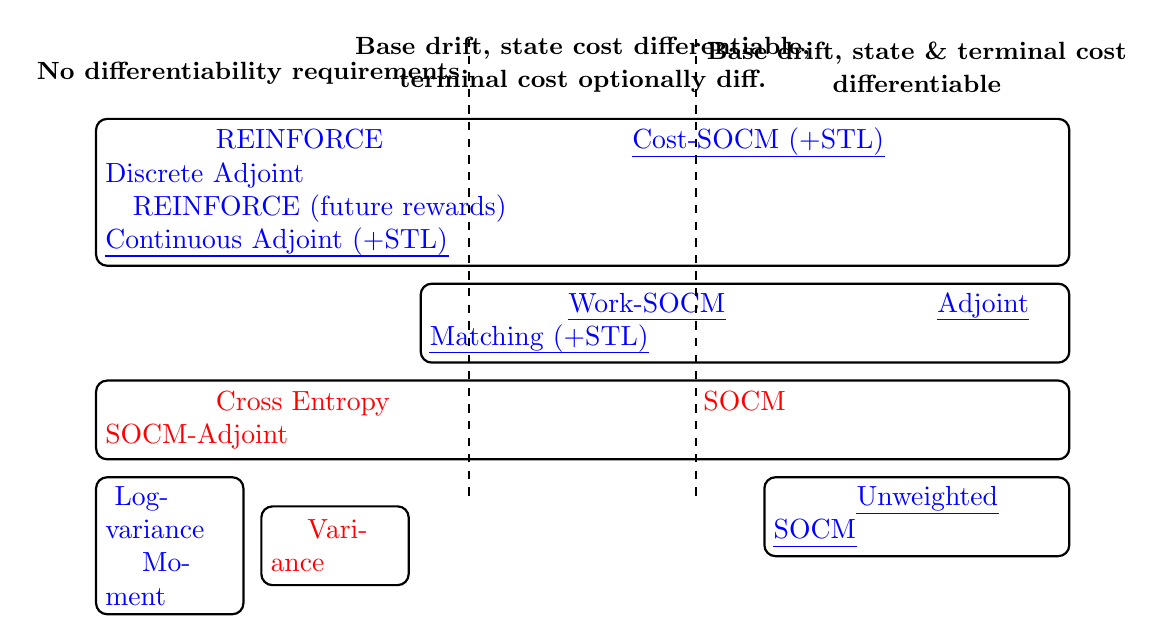
\begin{tikzpicture}[
    blocka/.style={draw, thick, text width=\textwidth, %align=center, 
    rectangle, rounded corners, minimum height=1cm},
    blockb/.style={draw, thick, text width=\textwidth, %align=center, 
    rectangle, rounded corners, minimum height=1cm},
    blockc/.style={draw, thick, text width=0.135\textwidth, align=left, 
    rectangle, rounded corners, minimum height=1cm},
    blockd/.style={draw, thick, text width=0.3\textwidth, align=center, 
    rectangle, rounded corners, minimum height=1cm},
    blocke/.style={draw, thick, text width=0.66\textwidth, %align=center, 
    rectangle, rounded corners, minimum height=1cm},
    blockf/.style={draw, thick, text width=0.3\textwidth, align=left, 
    rectangle, rounded corners, minimum height=1cm},
    line/.style={draw, thick, dashed},
    scalable/.style={text=blue},
    nonscalable/.style={text=red},
    node distance=0.5cm,
    label/.style={above=of groupA, align=center}
]

\node[blocka] (groupA) {
    \qquad\qquad\textcolor{blue}{REINFORCE} \qquad\qquad\qquad\qquad \ \ \textcolor{blue}{\uline{Cost-SOCM (+STL)}} \qquad\qquad\qquad\qquad \textcolor{blue}{Discrete Adjoint} \\ \quad \textcolor{blue}{REINFORCE (future rewards)} \qquad\qquad\qquad\qquad\qquad\qquad\qquad\qquad\qquad\quad 
    % \textcolor{blue}{SOCM+}
    \textcolor{blue}{\uline{Continuous Adjoint (+STL)}}
    % \qquad\qquad\qquad\qquad\qquad\qquad\qquad\quad \textcolor{blue}{Unweighted SOCM-adjoint}
};
\node[blocke, below=0.2cm of groupA.south east, anchor=north east] (groupA2) {
    \qquad\qquad\quad  \textcolor{blue}{\uline{Work-SOCM}} \qquad\qquad\qquad\quad \ \textcolor{blue}{\uline{Adjoint Matching (+STL)}} 
    % \\ \qquad\qquad\qquad\qquad\qquad\qquad\qquad\qquad\quad \textcolor{blue}{Work-SOCM+}
};
\node[blockb, below=0.2cm of groupA2.south east, anchor=north east] (groupB) {
    \qquad\qquad\textcolor{red}{Cross Entropy} \quad\qquad\qquad\qquad\qquad\qquad \textcolor{red}{SOCM} \qquad\qquad\qquad\qquad\qquad\qquad \textcolor{red}{SOCM-Adjoint}
};
\node[blockc, below=0.2cm of groupB.south west, anchor=north west] (groupC) {
    \ \textcolor{blue}{Log-variance} \\ \quad \  \textcolor{blue}{Moment}
};
\node[blockc, right=0.2cm of groupC] (groupE) {
    \quad \ \textcolor{red}{Variance}
};
% \node[blockd, right=of groupC] (groupD) {
% \node[blockc, below=0.2cm of groupB.south east, anchor=north east] (groupD) {
%     \qquad\textcolor{blue}{Unweighted SOCM}
% };
% \node[blocke, below=0.2cm of groupB.south east, anchor=north east] (groupD) {
%     \qquad\quad \ \textcolor{blue}{SOCM-Work} \qquad\qquad\quad \ \textcolor{blue}{Unweighted SOCM-Adjoint}
% };
\node[blockf, below=0.2cm of groupB.south east, anchor=north east] (groupF) {
    \qquad\quad \textcolor{blue}{\uline{Unweighted SOCM}}
};

% Labels for regions
\node[label] (labelA) at ([yshift=-0.2cm,xshift=-0.35\textwidth]groupA.north) {\small \textbf{No differentiability requirements}};
\node[label] (labelB) at ([yshift=-0.3cm]groupA.north) {\small \textbf{Base drift, state cost differentiable,} \\ \small \textbf{terminal cost optionally diff.}};
\node[label] (labelC) at ([yshift=-0.3cm,xshift=0.35\textwidth]groupA.north) {\small \textbf{Base drift, state \& terminal cost} \\  \small \textbf{differentiable}};

% Dashed lines to delimit regions
\draw[line] ([yshift=0.7cm,xshift=2.8cm]labelA.south) -- ([yshift=-5.1cm,xshift=2.8cm]labelA.south);
\draw[line] ([yshift=0.8cm,xshift=-2.8cm]labelC.south) -- ([yshift=-5.0cm,xshift=-2.8cm]labelC.south);

\end{tikzpicture}

\caption{Training losses for stochastic optimal control problems. Losses in blue scale to high-dimensions, while losses in red do not, as the gradient variance blows up exponentially with the dimension. By \autoref{thm:main}, losses in the same block (there are five different blocks) are equal in expectation, i.e. taking infinite batch size would yield the same gradient update. Novel losses are underlined, and losses that admit a Sticking The Landing version are identified with the suffix (+STL).}
\label{fig:SOC_taxonomy}
\end{figure}

The information in \autoref{thm:main} is summarized in \autoref{fig:SOC_taxonomy}. Additionally, the diagram contains information on the losses that require differentiating through the state and terminal costs, those that do not, and those that differentiate the state cost and may or may not differentiate the terminal costs. 
% (which are losses based on the path-wise reparameterization trick, where $M_t(T)$ can be set to zero to avoid computing $\nabla g$).  \brian{Is the path-wise reparameterization trick introduced somewhere?}

\section{Simple stochastic optimal control experiments} \label{sec:simple_exp}

We benchmark all the loss functions in our taxonomy in \autoref{fig:SOC_taxonomy} on four experimental settings where we have access to the ground truth optimal control, which means that we can compute the control $L^2$ error incurred by each algorithm throughout training. The settings are \textsc{Quadratic Ornstein Uhlenbeck, easy} and \textsc{hard}, and \textsc{Double Well, easy} and \textsc{hard}, and were used in \cite{domingoenrich2023stochastic,nüsken2023solving} (more details in \autoref{subsec:detail_exp}). 

\autoref{fig:control_L2_errors} contains all the plots; errors are averaged using an exponential moving average. The top left subfigure corresponds to an easy setting where all algorithms perform well. The best-performing losses are SOCM and UW-SOCM, which we introduce in \autoref{subsec:new_losses_app}. The top right subfigure is on a more challenging setting in which the running cost $f$ and the terminal cost $g$ are larger, where losses that do not scale well (those in red in \autoref{fig:SOC_taxonomy}) struggle. Larger costs make these losses fail completely, as gradient variance is too high. UW-SOCM achieves the lowest error. 

The bottom subfigures are for settings where the optimal process has 1024 modes. Algorithms need to explore all the modes, which is why the control $L^2$ errors decrease slower than in the top subfigures, and also the reason why some plots have occasional bounces. While Adjoint Matching achieves the lowest error in the bottom left subfigure, UW-SOCM is the best loss among those for which the error decreases monotonically. In the bottom right, UW-SOCM shows unstable behavior which we attribute to its weak theoretical guarantees (\autoref{prop:UW_SOCM_optimality}), and the best loss is SOCM.

In summary, while SOCM and UW-SOCM perform are the best loss functions in some settings, they struggle in others. In comparison, Continuous Adjoint and Adjoint Matching behave well across the board. 

\begin{figure}[H]
    \centering
    \includegraphics[width=0.495\textwidth]{toy_experiments/easy_EMA_norm_sqd_diff_optimal_7.png}
    \includegraphics[width=0.495\textwidth]{toy_experiments/hard_EMA_norm_sqd_diff_optimal_7.png}
    % \includegraphics[width=0.495\textwidth]{toy_experiments/linear_EMA_norm_sqd_diff_optimal_7.png}
    \includegraphics[width=0.495\textwidth]{toy_experiments/double_well_EMA_norm_sqd_diff_optimal_7.png}
    \includegraphics[width=0.495\textwidth]{toy_experiments/double_well_0.5_EMA_norm_sqd_diff_optimal_7.png}
    \caption{Control $L^2$ error incurred by each loss function throughout training, on four different settings.}
    \label{fig:control_L2_errors}
\end{figure}

\section{Diffusion fine-tuning experiments} \label{sec:diff_finetuning_exp}

% \begin{table}[h]
% \centering
% \begin{tabular}{lccccc}
%     \toprule
%     Fine-tuning loss & Inference $\sigma(t)$ & ImageReward & ClipScore & PickScore & Human Preference Score v2 
%      \\
%     \midrule
%     \multirow{2}{*}{None (Base Model)} & $\sqrt{2 \eta_t}$
%     & 
%     &  &  &  
%     \\ & 0
%     & 
%     &  &  & 
%     \\
%     \addlinespace
%     \multirow{2}{*}{Adjoint Matching} & $\sqrt{2 \eta_t}$
%     & 
%     &  &  &  
%     \\ & 0
%     & 
%     &  &  & 
%     \\
%     \addlinespace
%     \multirow{2}{*}{Continuous Adjoint} & $\sqrt{2 \eta_t}$
%     & 
%     &  &  &  
%     \\ & 0
%     & 
%     &  &  & 
%     \\
%     \addlinespace
%     \multirow{2}{*}{Discrete Adjoint} & $\sqrt{2 \eta_t}$
%     & 
%     &  &  &  
%     \\ & 0
%     & 
%     &  &  & 
%     \\
%     \addlinespace
%     ReFL $\sigma(t) = \sqrt{2 \eta_t}$ & $\sqrt{2 \eta_t}$
%     & 
%     &  &  &  
%     \\ ReFL $\sigma(t) = 0$ & 0
%     & 
%     &  &  & 
%     \\
%     \addlinespace
%     Draft-1 $\sigma(t) = \sqrt{2 \eta_t}$ & $\sqrt{2 \eta_t}$
%     & 
%     &  &  &  
%     \\ Draft-1 $\sigma(t) = 0$ & 0
%     & 
%     &  &  & 
%     \\
%     \addlinespace
%     Draft-40 $\sigma(t) = \sqrt{2 \eta_t}$ & $\sqrt{2 \eta_t}$
%     & 
%     &  &  &  
%     \\ Draft-40 $\sigma(t) = 0$ & 0
%     & 
%     &  &  & 
%     \bottomrule
% \end{tabular}
% \caption{TODO
% }
% \label{table:coefficients}
% \end{table}

\begin{table}[h]
\centering
{\footnotesize
\begin{tabular}{lccccccc}
    \toprule
    FT Loss & FT $\sigma(t)$ & Inf. $\sigma(t)$ & ImageReward ($\uparrow$) & ClipScore ($\uparrow$) & PickScore ($\uparrow$) & HPS v2 ($\uparrow$) & Seconds/it.  \\
    \midrule
    \multirow{2}{*}{None (Base)} & \multirow{2}{*}{N/A}& $\sqrt{2 \eta_t}$ & $-1.356 \pm 0.007$ & $24.33 \pm 0.11$ & $17.28 \pm 0.02$ & $16.30 \pm 0.04$ & \multirow{2}{*}{N/A} \\
                                 &                     & 0                 & $-0.898 \pm 0.012$ & $28.46 \pm 0.05$ & $18.18 \pm 0.02$ & $17.94 \pm 0.05$ & \\
    \addlinespace
    \multirow{2}{*}{ReFL}              & $\sqrt{2 \eta_t}$ & $\sqrt{2 \eta_t}$ & $-0.379 \pm 0.010$ & $27.47 \pm 0.07$ & $18.39 \pm 0.03$ & $20.65 \pm 0.02$ & $23.5 \pm 1.0$ \\
                                       & 0                 & 0                 & $-0.303 \pm 0.095$ & $29.13 \pm 0.34$ & $18.76 \pm 0.14$ & $20.71 \pm 0.34$ & $24.6 \pm 1.3$ \\
    \addlinespace
    \multirow{2}{*}{Draft-1}           & $\sqrt{2 \eta_t}$ & $\sqrt{2 \eta_t}$ & $-0.200 \pm 0.029$ & $27.89 \pm 0.12$ & $18.59 \pm 0.03$ & $21.39 \pm 0.08$ & $34.1 \pm 0.1$ \\
                                       & 0                 & 0                 & $-0.188 \pm 0.034$ & $29.56 \pm 0.07$ & $18.94 \pm 0.01$ & $21.15 \pm 0.09$ & $37.7 \pm 0.3$ \\
    \addlinespace
    \multirow{2}{*}{Draft-40}          & $\sqrt{2 \eta_t}$ & $\sqrt{2 \eta_t}$ & $-0.648 \pm 0.170$ & $28.16 \pm 0.73$ & $18.42 \pm 0.73$ & $19.54 \pm 0.86$ & $99.0 \pm 2.7$ \\
                                       & 0                 & 0                 & $-0.208 \pm 0.067$ & $29.84 \pm 0.14$ & $19.09 \pm 0.04$ & $21.66 \pm 0.23$ & $105.1 \pm 1.8$ \\
    \addlinespace
    \multirow{2}{*}{Adj. Matching}  & \multirow{2}{*}{$\sqrt{2 \eta_t}$} & $\sqrt{2 \eta_t}$ & $\mathbf{0.157} \pm 0.024$ & $29.58 \pm 0.19$ & $19.18 \pm 0.06$ & $\mathbf{23.16} \pm 0.12$ & \multirow{2}{*}{$150.7 \pm 2.0$} \\
                                    &                                    & 0                 & $0.069 \pm 0.003$ & $\mathbf{30.59} \pm 0.05$ & $\mathbf{19.47} \pm 0.04$ & $22.33 \pm 0.03$ &  \\
    \addlinespace
    \multirow{2}{*}{Cont. Adjoint}  & \multirow{2}{*}{$\sqrt{2 \eta_t}$} & $\sqrt{2 \eta_t}$ & $-0.240 \pm 0.022$ & $28.75 \pm 0.03$ & $18.84 \pm 0.03$ & $21.80 \pm 0.14$ & \multirow{2}{*}{$202.5 \pm 3.1$} \\
                                    &                                    & 0                 & $-0.214 \pm 0.018$ & $30.13 \pm 0.12$ & $19.25 \pm 0.03$ & $21.47 \pm 0.15$ &  \\
    \addlinespace
    \multirow{2}{*}{Disc. Adjoint}  & \multirow{2}{*}{$\sqrt{2 \eta_t}$} & $\sqrt{2 \eta_t}$ & $-0.530 \pm 0.154$ & $28.27 \pm 0.52$ & $18.47 \pm 0.18$ & $20.40 \pm 0.77$ & \multirow{2}{*}{$ 144.6 \pm 1.3$} \\
                                    &                                    & 0                 & $-0.615 \pm 0.124$ & $29.07 \pm 0.48$ & $18.75 \pm 0.13$ & $19.60 \pm 0.63$ &  \\
    \bottomrule
\end{tabular}
}
\caption{Performance metrics for various fine-tuning methods for \textit{multi-prompt} text-to-image generation. The second and third columns show the noise schedules $\sigma(t)$ used for fine-tuning and for inference: $\sigma(t) = \sqrt{2\eta_t}$ corresponds to Memoryless Flow Matching \eqref{eq:memoryless_FM_sde}, and $\sigma(t) = 0$ to the Flow Matching ODE \eqref{eq:FM_ode}. Confidence intervals show standard errors of estimates; computed over 3 runs of the fine-tuning algorithm on separate fine-tuning prompt datasets of size 20000 each. Test prompt sets are of size 1000, and also different for each run.}
\label{table:metrics_multiprompt}
\end{table}

\begin{table}[h]
\centering
{\small
\begin{tabular}{lccccccc}
    \toprule
    FT Loss & FT $\sigma(t)$ & Inference $\sigma(t)$ & ImageReward$\, \uparrow$ & ClipScore$\, \uparrow$ & PickScore$\, \uparrow$ & HPS v2$\, \uparrow$ \\
    \midrule
    \multirow{2}{*}{None (Base)} & \multirow{2}{*}{N/A}& $\sqrt{2 \eta_t}$ & $-1.356 \pm 0.032$ & $24.33 \pm 0.21$ & $17.28 \pm 0.06$ & $16.30 \pm 0.14$ \\
                                 &                     & 0                 & $-0.898 \pm 0.037$ & $28.46 \pm 0.17$ & $18.18 \pm 0.06$ & $17.94 \pm 0.14$ \\
    \addlinespace
    \multirow{2}{*}{ReFL}              & $\sqrt{2 \eta_t}$ & $\sqrt{2 \eta_t}$ & $0.703 \pm 0.045$ & $29.12 \pm 0.39$ & $18.72 \pm 0.20$ & $22.20 \pm 0.54$ \\
                                       & 0                 & 0                 & N/A & N/A & N/A & N/A \\
    \addlinespace
    \multirow{2}{*}{Draft-1}           & $\sqrt{2 \eta_t}$ & $\sqrt{2 \eta_t}$ & $\mathbf{1.111} \pm 0.056$ & $30.44 \pm 0.26$ & $19.27 \pm 0.07$ & $24.11 \pm 0.32$  \\
                                       & 0                 & 0                 & $1.060 \pm 0.080$ & $30.93 \pm 0.23$ & $19.25 \pm 0.11$ & $23.53 \pm 0.30$ \\
    \addlinespace
    \multirow{2}{*}{Draft-40}          & $\sqrt{2 \eta_t}$ & $\sqrt{2 \eta_t}$ & $-1.212 \pm 0.442$ & $23.31 \pm 2.54$ & $17.38 \pm 0.73$ & $14.96 \pm 3.54$  \\
                                       & 0                 & 0                 & $-0.434 \pm 0.278$ & $27.36 \pm 1.10$ & $18.47 \pm 0.31$ & $20.34 \pm 1.61$ \\
    \addlinespace
    Adj.-Matching  & \multirow{2}{*}{$\sqrt{2 \eta_t}$} & $\sqrt{2 \eta_t}$ & $0.356 \pm 0.100$ & $29.90 \pm 0.61$ & $19.12 \pm 0.14$ & $23.51 \pm 0.28$ \\
    $\beta = 1000$                     &                                    & 0                 & $0.266 \pm 0.080$ & $30.92 \pm 0.29$ & $19.39 \pm 0.09$ & $22.82 \pm 0.24$ \\
    \addlinespace
    Adj.-Matching & \multirow{2}{*}{$\sqrt{2 \eta_t}$} & $\sqrt{2 \eta_t}$ & $0.484 \pm 0.067$ & $29.96 \pm 0.27$ & $19.17 \pm 0.10$ & $23.81 \pm 0.25$ \\
    $\beta = 2500$                     &                                    & 0                 & $0.413 \pm 0.068$ & $31.19 \pm 0.25$ & $19.48 \pm 0.09$ & $23.35 \pm 0.31$ \\
    \addlinespace
    Adj.-Matching  & \multirow{2}{*}{$\sqrt{2 \eta_t}$} & $\sqrt{2 \eta_t}$ & $0.610 \pm 0.078$ & $29.68 \pm 0.46$ & $19.24 \pm 0.10$ & $\mathbf{24.20} \pm 0.16$ \\
    $\beta = 12500$                    &                                    & 0                 & $0.569 \pm 0.062$ & $\mathbf{31.18} \pm 0.21$ & $\mathbf{19.62} \pm 0.08$ & $23.88 \pm 0.23$ \\
    \bottomrule
\end{tabular}
}
\caption{Consistency metrics for various fine-tuning methods for \textit{multi-prompt} text-to-image generation. The second and third columns show the noise schedules $\sigma(t)$ used for fine-tuning and for inference: $\sigma(t) = \sqrt{2\eta_t}$ corresponds to Memoryless Flow Matching \eqref{eq:memoryless_FM_sde}, and $\sigma(t) = 0$ to the Flow Matching ODE \eqref{eq:FM_ode}. Confidence intervals show standard errors of estimates; computed over 3 runs of the fine-tuning algorithm on separate fine-tuning prompt datasets of size 20000 each. Test prompt sets are of size 1000, and also different for each run. \textcolor{red}{Separate ImageReward with line. Have ClipScore, HPS v2, DreamSim in the main paper, others in appendix.}.}
\label{table:metrics_multiprompt}
\end{table}

\begin{table}[h]
\centering
{\small
\begin{tabular}{lccccccc}
    \toprule
    FT Loss & FT $\sigma(t)$ & Inference $\sigma(t)$ & DreamSim diversity$\, \uparrow$ & ClipScore diversity$\, \uparrow$ & PickScore diversity$\, \uparrow$ \\
    \midrule
    \multirow{2}{*}{None (Base)} & \multirow{2}{*}{N/A} & $\sqrt{2 \eta_t}$ & $53.46 \pm 0.53$ & $28.65 \pm 0.53$ & $1.62 \pm 0.02$ \\
                                 &                     & 0                 & $56.24 \pm 1.47$ & $29.77 \pm 1.42$ & $1.83 \pm 0.09$ \\
    \addlinespace
    \multirow{2}{*}{ReFL}              & $\sqrt{2 \eta_t}$ & $\sqrt{2 \eta_t}$ & $32.33 \pm 1.48$ & $18.95 \pm 1.20$ & $1.39 \pm 0.13$ \\
                                       & 0                 & 0                 & N/A & N/A & N/A \\
    \addlinespace
    \multirow{2}{*}{Draft-1}           & $\sqrt{2 \eta_t}$ & $\sqrt{2 \eta_t}$ & $28.79 \pm 1.21$ & $16.15 \pm 0.73$ & $1.31 \pm 0.12$ \\
                                       & 0                 & 0                 & $29.79 \pm 0.85$ & $16.13 \pm 0.95$ & $1.32 \pm 0.07$  \\
    \addlinespace
    \multirow{2}{*}{Draft-40}          & $\sqrt{2 \eta_t}$ & $\sqrt{2 \eta_t}$ & $29.06 \pm 14.99$ & $16.63 \pm 7.67$ & $1.22 \pm 0.53$ \\
                                       & 0                 & 0                 &  $40.10 \pm 3.58$ & $22.10 \pm 2.29$ & $1.60 \pm 0.11$ \\
    \addlinespace
    Adj.-Matching  & \multirow{2}{*}{$\sqrt{2 \eta_t}$} & $\sqrt{2 \eta_t}$ & $40.88 \pm 2.86$ & $21.42 \pm 1.43$ & $1.66 \pm 0.09$ \\
    $\beta = 1000$                     &                                    & 0                 & $43.65 \pm 2.16$ & $21.54 \pm 1.20$ & $1.78 \pm 0.09$ \\
    \addlinespace
    Adj.-Matching & \multirow{2}{*}{$\sqrt{2 \eta_t}$} & $\sqrt{2 \eta_t}$ & $39.49 \pm 1.57$ & $21.48 \pm 1.37$ & $1.71 \pm 0.09$ \\
    $\beta = 2500$                     &                                    & 0                 & $41.71 \pm 1.63$ & $20.59 \pm 1.31$ & $1.76 \pm 0.10$ \\
    \addlinespace
    Adj.-Matching  & \multirow{2}{*}{$\sqrt{2 \eta_t}$} & $\sqrt{2 \eta_t}$ & $36.30 \pm 2.72$ & $20.38 \pm 1.78$ & $1.68 \pm 0.13$ \\
    $\beta = 12500$                    &                                    & 0                 & $37.95 \pm 2.25$ & $19.49 \pm 1.47$ & $1.71 \pm 0.12$ \\
    \bottomrule
\end{tabular}
}
\caption{Diversity metrics for various fine-tuning methods for \textit{multi-prompt} text-to-image generation. The second and third columns show the noise schedules $\sigma(t)$ used for fine-tuning and for inference: $\sigma(t) = \sqrt{2\eta_t}$ corresponds to Memoryless Flow Matching \eqref{eq:memoryless_FM_sde}, and $\sigma(t) = 0$ to the Flow Matching ODE \eqref{eq:FM_ode}. Confidence intervals show standard errors of estimates; computed over 3 runs of the fine-tuning algorithm on separate fine-tuning prompt datasets of size 20000 each. Test prompt sets are of size 1000, and also different for each run. \textcolor{red}{Merge Dreamsim into the first table, leave other metrics in the appendix.}}
\label{table:metrics_multiprompt}
\end{table}

\begin{table}[h]
\centering
{\footnotesize
\begin{tabular}{lccccccc}
    \toprule
    FT Loss & FT $\sigma(t)$ & Inf. $\sigma(t)$ & ImageReward ($\uparrow$) & ClipScore ($\uparrow$) & PickScore ($\uparrow$) & HPS v2 ($\uparrow$) \\
    \midrule
    \multirow{2}{*}{None (Base)} & \multirow{2}{*}{N/A}& $\sqrt{2 \eta_t}$ & $-0.858 \pm 0.015$ & $29.80 \pm 0.11$ & $17.72 \pm \num{1e-3}$ & $19.35 \pm 0.02$ \\
                                 &                     & 0                 & $-0.061 \pm 0.018$ & $34.03 \pm 0.06$ & $18.75 \pm 0.02$ & $21.23 \pm 0.10$ \\
    \addlinespace
    \multirow{2}{*}{ReFL}              & $\sqrt{2 \eta_t}$ & $\sqrt{2 \eta_t}$ & $1.359 \pm 0.029$ & $36.86 \pm 0.05$ & $19.51 \pm 0.04$ & $26.24 \pm 0.20$ \\
                                       & 0                 & 0                 & $1.340 \pm 0.106$ & $37.39 \pm 0.22$ & $19.86 \pm 0.11$ & $25.80 \pm 0.45$ \\
    \addlinespace
    \multirow{2}{*}{Draft-1}           & $\sqrt{2 \eta_t}$ & $\sqrt{2 \eta_t}$ & $1.783 \pm 0.013$ & $37.83 \pm 0.06$ & $19.97 \pm 0.07$ & $28.86 \pm 0.15$ \\
                                       & 0                 & 0                 & $1.542 \pm 0.048$ & $37.93 \pm 0.12$ & $19.93 \pm 0.06$ & $26.48 \pm 0.29$ \\
    \addlinespace
    \multirow{2}{*}{Draft-40}          & $\sqrt{2 \eta_t}$ & $\sqrt{2 \eta_t}$ & $1.496 \pm 0.138$ & $37.60 \pm 0.76$ & $19.88 \pm 0.28$ & $27.36 \pm 0.52$ \\
                                       & 0                 & 0                 & $\mathbf{1.836} \pm 0.070$ & $\mathbf{38.92} \pm 0.43$ & $\mathbf{20.53} \pm 0.11$ & $\mathbf{29.33} \pm 0.69$ \\
    \addlinespace
    \multirow{2}{*}{Adj. Matching}  & \multirow{2}{*}{$\sqrt{2 \eta_t}$} & $\sqrt{2 \eta_t}$ & $\mathbf{1.820} \pm 0.014$ & $38.31 \pm 0.26$ & $\mathbf{20.40} \pm 0.10$ & $\mathbf{29.00} \pm 0.47$ \\
                                    &                                    & 0                 & $1.719 \pm 0.028$ & $\mathbf{38.59} \pm 0.22$ & $20.24 \pm 0.05$ & $28.60 \pm 0.46$ \\
    \addlinespace
    \multirow{2}{*}{Cont. Adjoint}  & \multirow{2}{*}{$\sqrt{2 \eta_t}$} & $\sqrt{2 \eta_t}$ & $1.791 \pm 0.008$ & $38.18 \pm 0.28$ & $\mathbf{20.46} \pm 0.05$ & $\mathbf{29.19} \pm 0.09$ \\
                                    &                                    & 0                 & $1.684 \pm 0.033$ & $\mathbf{38.57} \pm 0.16$ & $20.31 \pm 0.09$ & $28.72 \pm 0.33$ \\
    \addlinespace
    \multirow{2}{*}{Disc. Adjoint}  & \multirow{2}{*}{$\sqrt{2 \eta_t}$} & $\sqrt{2 \eta_t}$ & $1.571 \pm 0.070$ & $37.31 \pm 0.53$ & $20.08 \pm 0.12$ & $28.29 \pm 0.33$ \\
                                    &                                    & 0                 & $1.563 \pm 0.022$ & $38.11 \pm 0.26$ & $20.09 \pm 0.06$ & $28.51 \pm 0.38$ \\
    \bottomrule
\end{tabular}
}
\caption{Performance metrics for various fine-tuning methods for \textit{single prompt} text-to-image generation, with prompt: “\textit{Parrot on sandy beach near sea. Beach holiday background.}”. The second and third columns show the noise schedules $\sigma(t)$ used for fine-tuning and for inference: $\sigma(t) = \sqrt{2\eta_t}$ corresponds to Memoryless Flow Matching \eqref{eq:memoryless_FM_sde}, and $\sigma(t) = 0$ to the Flow Matching ODE \eqref{eq:FM_ode}. Confidence intervals show standard errors of estimates; computed over 3 runs of the fine-tuning algorithm on separate fine-tuning prompt datasets of size 20000 each. Test prompt sets are of size 1000, and also different for each run.}
\label{table:metrics_single_prompt}
\end{table}

\textcolor{red}{Plots for all baselines and our best method, and then plots for all SOC algorithms}

\textcolor{red}{Add (Control + Reward)/(Reward only) after method name in label} 
\textcolor{red}{Remove plot titles}
\textcolor{red}{Not putting figure title on Python, but on subfigure framework in Latex}

\begin{figure}
    \centering    \includegraphics[width=0.495\textwidth]{text-to-image_experiments/multiprompt_plots_2/multiprompt_control_objective_plot.png}
    \includegraphics[width=0.495\textwidth]{text-to-image_experiments/multiprompt_plots_2/multiprompt_control_term_plot.png}
    \includegraphics[width=0.495\textwidth]{text-to-image_experiments/multiprompt_plots_2/multiprompt_reward_plot.png}
    \includegraphics[width=0.495\textwidth]{text-to-image_experiments/multiprompt_plots_2/multiprompt_clipscore_plot.png}
    \caption{Error bars show standard errors of estimates; computed over 3 runs of the fine-tuning algorithm on separate fine-tuning prompt datasets of size 20000 each. Test prompt sets are of size 1000, and also different for each run.}
    \label{fig:enter-label}
\end{figure}

\begin{figure}
    \centering
    \includegraphics[width=0.995\textwidth]{text-to-image_experiments/multiprompt_images_1/figure_1_10_None_0.0.jpg}
    \includegraphics[width=0.995\textwidth]{text-to-image_experiments/multiprompt_images_1/figure_1_10_adjoint_matching_1.0.jpg}
    \includegraphics[width=0.995\textwidth]{text-to-image_experiments/multiprompt_images_1/figure_1_10_adjoint_matching_0.0.jpg}
    \includegraphics[width=0.995\textwidth]{text-to-image_experiments/multiprompt_images_1/figure_1_10_cont_adjoint_0.0.jpg}
    \includegraphics[width=0.995\textwidth]{text-to-image_experiments/multiprompt_images_1/figure_1_10_discrete_adjoint_0.0.jpg}
    \includegraphics[width=0.995\textwidth]{text-to-image_experiments/multiprompt_images_1/figure_1_10_refl_0.0.jpg}
    \includegraphics[width=0.995\textwidth]{text-to-image_experiments/multiprompt_images_1/figure_1_10_draft-1_0.0.jpg}
    \includegraphics[width=0.995\textwidth]{text-to-image_experiments/multiprompt_images_1/figure_1_10_draft-40_0.0.jpg}
    \caption{Caption}
    \label{fig:enter-label}
\end{figure}

% \begin{figure}
%     \centering
%     \includegraphics[width=0.495\textwidth]{text-to-image_experiments/multiprompt_images_0/multiprompt_step_0.png}
%     \includegraphics[width=0.495\textwidth]{text-to-image_experiments/multiprompt_images_0/multiprompt_work_adjoint_step_450.png}
%     \includegraphics[width=0.495\textwidth]{text-to-image_experiments/multiprompt_images_0/multiprompt_draft-1_step_450.png}
%     \includegraphics[width=0.495\textwidth]{text-to-image_experiments/multiprompt_images_0/multiprompt_draft-40_step_450.png}
%     \caption{Caption}
%     \label{fig:enter-label}
% \end{figure}

% \begin{figure}
%     \centering
%     \includegraphics[width=0.495\textwidth]{text-to-image_experiments/single_prompt_plots_0/single_prompt_control_objective_plot.png}
%     \includegraphics[width=0.495\textwidth]{text-to-image_experiments/single_prompt_plots_0/single_prompt_control_term_plot.png}
%     \includegraphics[width=0.495\textwidth]{text-to-image_experiments/single_prompt_plots_0/single_prompt_reward_plot.png}
%     \includegraphics[width=0.495\textwidth]{text-to-image_experiments/single_prompt_plots_0/single_prompt_clipscore_plot.png}
%     \caption{Caption}
%     \label{fig:enter-label}
% \end{figure}

\begin{figure}
    \centering
    \includegraphics[width=0.495\textwidth]{text-to-image_experiments/single_prompt_plots_1/single_prompt_74488_control_objective_plot.png}
    \includegraphics[width=0.495\textwidth]{text-to-image_experiments/single_prompt_plots_1/single_prompt_74488_control_term_plot.png}
    \includegraphics[width=0.495\textwidth]{text-to-image_experiments/single_prompt_plots_1/single_prompt_74488_reward_plot.png}
    \includegraphics[width=0.495\textwidth]{text-to-image_experiments/single_prompt_plots_1/single_prompt_74488_clipscore_plot.png}
    \caption{Caption}
    \label{fig:enter-label}
\end{figure}

\begin{figure}
    \centering
    \includegraphics[width=0.495\textwidth]{text-to-image_experiments/single_prompt_images_0/single_prompt_step_0.png}
    \includegraphics[width=0.495\textwidth]{text-to-image_experiments/single_prompt_images_0/single_prompt_work_adjoint_step_450.png}
    \includegraphics[width=0.495\textwidth]{text-to-image_experiments/single_prompt_images_0/single_prompt_draft-1_step_450.png}
    \includegraphics[width=0.495\textwidth]{text-to-image_experiments/single_prompt_images_0/single_prompt_draft-40_step_450.png}
    \caption{Prompt: "Beautiful brunette little girl wearing casual sweater praying with hands together asking for forgiveness smiling confident."}
    \label{fig:enter-label}
\end{figure}

\begin{figure}
    \centering
    \includegraphics[width=0.995\textwidth]{text-to-image_experiments/single_prompt_images_1/74488_figure_1_10_None_0.0.jpg}
    \includegraphics[width=0.995\textwidth]{text-to-image_experiments/single_prompt_images_1/74488_figure_1_10_adjoint_matching_1.0.jpg}
    \includegraphics[width=0.995\textwidth]{text-to-image_experiments/single_prompt_images_1/74488_figure_1_10_adjoint_matching_0.0.jpg}
    \includegraphics[width=0.995\textwidth]{text-to-image_experiments/single_prompt_images_1/74488_figure_1_10_cont_adjoint_0.0.jpg}
    \includegraphics[width=0.995\textwidth]{text-to-image_experiments/single_prompt_images_1/74488_figure_1_10_discrete_adjoint_0.0.jpg}
    \includegraphics[width=0.995\textwidth]{text-to-image_experiments/single_prompt_images_1/74488_figure_1_10_refl_0.0.jpg}
    \includegraphics[width=0.995\textwidth]{text-to-image_experiments/single_prompt_images_1/74488_figure_1_10_draft-1_0.0.jpg}
    \includegraphics[width=0.995\textwidth]{text-to-image_experiments/single_prompt_images_1/74488_figure_1_10_draft-40_0.0.jpg}
    \caption{Prompt: “Parrot on sandy beach near sea. Beach holiday background.”}
    \label{fig:enter-label}
\end{figure}

\section{Conclusion}
\label{sec:conclusion}

\clearpage
\newpage
\bibliographystyle{assets/plainnat}
\bibliography{biblio}

\clearpage
\newpage
\beginappendix

\section{Appendix} \label{appendix}


\subsection{NewYorker Data for evaluation}

\begin{figure}[!ht]
\small
\centering
\includegraphics[width=0.4\textwidth]{figures/length.png}
\caption{\label{lengthdist} Distribution of word count of stories in our test set}
\end{figure}

Table \ref{teststories} shows the data used for conducting our evaluation. The 12 stories shown are taken from The New Yorker and summarized into single-sentence plots. These stories come from highly established literary experts acting as an upper bound for what it means to be creative. These stories span complex themes.

\begin{table*}[!ht]
\centering
\small
\def\arraystretch{1.35}
\begin{tabular}{|l|}
\hline
\begin{tabular}[c]{@{}l@{}}Write a New Yorker-style story given the plot below. Make sure it is atleast \textbf{\color{blue}\{\{word\_count\}\}} words. Directly start with the\\ story, do not say things like `Here's the story {[}...{]}:\end{tabular}                                                                                                                                                                                            \\ \hline\hline
\begin{tabular}[c]{@{}l@{}}You wrote the story I gave you below. I requested a story with \textbf{\color{blue}\{\{word\_count\}\}} words, but the story only has\\ \textbf{\color{blue}\{\{current\_word\_count\}\}} words. Can you rewrite the story to make it longer, and closer to the \textbf{\color{blue}\{\{word\_count\}\}} word target\\ I gave you. Directly start with the story, do not say things like `Here's the story {[}...{]}:`\\ \\ Current story: \{\{story\}\}\end{tabular} \\ \hline
\end{tabular}
\vspace{2ex}
\caption{\label{promptstory}Prompt to write the initial story (Row1) vs Prompt to rewrite the initial story to be longer. word\_count represents the number of words in the human written story on a given plot (P) while current\_word\_count represents the number of words in the LLM generated story on the same plot (P)}
\end{table*}

\begin{table*}[!ht]
\def\arraystretch{1.15}
\small
\begin{tabular}{|l|l|}
\hline
Story                                    & Plot                                                                                                                                                                                                                                                                                                                                                                                                                                                                                                                                   \\ \hline
\href{https://www.newyorker.com/books/flash-fiction/a-triangle}{A Triangle}                               & \begin{tabular}[c]{@{}l@{}}An observer becomes entranced by a seemingly ordinary couple on the street, follows them home, and then \\watches them from outside in the rising floodwaters, drawing an eerie connection between the woman and\\ a discarded, burned chair they'd noticed earlier.\end{tabular}                                                                                                                                                                    \\ \hline\hline
\href{https://www.newyorker.com/books/flash-fiction/barbara-detroit-1966}{\begin{tabular}[c]{@{}l@{}}Barbara\\ Detroit,1966\end{tabular}}                    & \begin{tabular}[c]{@{}l@{}}On Feb 12, 1966, a heavily pregnant woman named Barbara experienced a shocking incident in her synagogue\\in Southfield, Detroit, where a young man shot and killed the renowned Rabbi Adler before turning the gun\\ on himself, and though Barbara tried to reach the shooter, she was swept away by the fleeing crowd.\end{tabular}                                                                              \\ \hline\hline
\href{https://www.newyorker.com/books/flash-fiction/beyond-nature}{Beyond Nature}                           & \begin{tabular}[c]{@{}l@{}}A solitary man walking in a remote mountainous region comes across a car crash, and stays by the side\\ of the lifeless female victim, narrating stories of his past and reflecting on the impermanence of \\events and life itself, while awaiting emergency services amidst the looming presence of wilderness.\end{tabular}                                                                                                                \\ \hline\hline
\href{https://www.newyorker.com/books/flash-fiction/certain-european-movies}{\begin{tabular}[c]{@{}l@{}}Certain European\\ Movies\end{tabular}}                  & \begin{tabular}[c]{@{}l@{}}Two individuals, at a residency together, navigate the complexity of their ephemeral relationship during\\ their final beach trip, framed by misadventures, subtle tensions, unspoken desires, and looming departures.\end{tabular}                                                                                                                                                                                   \\ \hline\hline
\href{https://www.newyorker.com/books/flash-fiction/keys}{Keys}                                     & \begin{tabular}[c]{@{}l@{}}Daniel, struggling with recurring dreams of his ex-wife Rachel and a mysterious unused flat, eventually \\discusses them with his current partner Isabel, sparking various reflections and conversations about their\\ past relationships, until a real-life discovery of old keys triggers a nostalgic memory and helps him find a\\ way to reconnect with his present relationship through canoeing.\end{tabular}                                     \\ \hline\hline
\href{https://www.newyorker.com/books/flash-fiction/listening-for-the-click}{\begin{tabular}[c]{@{}l@{}}Listening For\\ the Click\end{tabular}}                  & \begin{tabular}[c]{@{}l@{}}Navigating a complex social landscape, the protagonist experiences a series of complex relationships \\and emotional turmoil in a student environment, and engages in self-discovery and self-reflection as she\\ interacts with the characters Carl, Martin, Lizzy, and Johan, resulting in a journey of introspection,\\ betrayal, love, and personal growth.\end{tabular}                                                          \\ \hline\hline
\href{https://www.newyorker.com/magazine/2023/05/15/maintenance-hvidovre-fiction-olga-ravn}{\begin{tabular}[c]{@{}l@{}}Maintenance,\\ Hvidovre\end{tabular}}                   & \begin{tabular}[c]{@{}l@{}}A woman experiences a disorienting night in a maternity ward where she encounters other similarly \\disoriented new mothers, leading to an uncanny mix-up where she leaves the hospital with a baby \\that she realizes is not her own, yet accepts the situation with an inexplicable sense of happiness.\end{tabular}                                                                                                  \\ \hline\hline
\href{https://www.newyorker.com/magazine/2022/11/14/returns}{Returns}                                  & \begin{tabular}[c]{@{}l@{}}The narrator visits their elderly mother in her small town, spending a day with her that is filled with \\nostalgia, conversation, and old habits, only to return a month later after her hospitalization due to\\ a sunstroke, finding remnants of their last visit.\end{tabular}                                                                                                                                                                      \\ \hline\hline
\href{https://www.newyorker.com/books/flash-fiction/the-facade-renovation-thats-going-well}{\begin{tabular}[c]{@{}l@{}}The Facade \\Renovation\\ That’s Going Well\end{tabular}} & \begin{tabular}[c]{@{}l@{}}An academic faculty housed in a building with a critical waterproofing layer missing experiences a series\\ of disruptive and problematic construction repairs, causing tension, inconvenience, and health concerns\\ among the tenants, ultimately leading to resignation and endurance in hopes of better future circumstances.\end{tabular}                                                        \\ \hline\hline
\href{https://www.newyorker.com/books/flash-fiction/the-kingdom-that-failed}{\begin{tabular}[c]{@{}l@{}}The Kingdom\\ That Failed\end{tabular}}                  & \begin{tabular}[c]{@{}l@{}}The narrator recounts their college friendship with the seemingly flawless Q, and after a decade apart, \\they accidentally cross paths at a pool, where the narrator anonymously observes Q's failed attempt to \\let down a woman about a work-related issue, demonstrating that Q, too, has his share of difficulties.\end{tabular}                                                                                                \\ \hline\hline
\href{https://www.newyorker.com/magazine/2022/06/13/trash }{Trash}                                    & \begin{tabular}[c]{@{}l@{}}A woman unexpectedly marries the son of a successful, ambitious woman named Miss Emily, finding both \\acceptance and critique from her mother-in-law as she navigates this new relationship and confronts the \\stark contrasts between her former life as a supermarket cashier and her new life as part of a well-off family.\end{tabular}                                                                                                            \\ \hline\hline
\href{https://www.newyorker.com/culture/personal-history/the-last-dance-with-my-dad}{\begin{tabular}[c]{@{}l@{}}The Last Dance\\ with my Dad \end{tabular}}               & \begin{tabular}[c]{@{}l@{}}A young teenager recounts her experiences of fitting into her father's gay lifestyle, highlighted by a\\ seven-day cruise with hundreds of gay men, where she experienced acceptance and connection, had her\\ first genuine interaction with a  boy, and shared a last dance with her terminally ill father.\end{tabular}                                                                                                       \\ \hline
\end{tabular}
\vspace{2ex}
\caption{\label{teststories} Expert-written short stories from the New Yorker along with their human-verified GPT4 generated summary as plots that are included as part of our test data for Creativity Evaluation}
\end{table*}


\subsection{Expert Perception on the TTCW tests}

\begin{figure*}[!ht]
    \centering
     \includegraphics[width=\textwidth]{figures/rel.pdf}
    \caption{\label{relev} Relative Evaluation by Creative Writing Experts within a given group of four stories}
\end{figure*}

\begin{table*}[!ht]
\small
\centering
\begin{tabular}{|l|l|}
\hline
E5 & \begin{tabular}[c]{@{}l@{}}It was a pretty effective rubric! I'm used to being more subjective in my work -- did you like a story? Did it connect with \\you? Did it make sense? Why or why not? It was often challenging to break it down into more regimented segments \\like the rubric asked for -- but I do think that it allowed me to express the subjective feelings in a pretty thorough and\\ structured way!\end{tabular}                                                                                                                                                                 \\ \hline
E3 & \begin{tabular}[c]{@{}l@{}}As for the rubric, I thought it was quite thorough. There were some categories where I would say the story didn’t ``pass,"\\ but which were excellent. This happened often with the categories about multiple points of view, and innovative\\ structure and form. Overall, I think the rubric was helpful in helping me think about the different aspects of storytelling.\end{tabular}                                                                                                                                                                                 \\ \hline
E4 & \begin{tabular}[c]{@{}l@{}}I thought the rubric felt pretty thorough; the only part I felt could be added was that suggestion about consistency in\\ voice \& diction!\end{tabular}                                                                                                                                                         \\ \hline
E2 & \begin{tabular}[c]{@{}l@{}}The rubric seemed great to me! It’s however hard to talk about something like pacing without talking about scene and \\summary, for instance. Or the difference between originality of thought and originality in theme/content—wouldn’t the \\latter make up the former and vice/versa? But it is also comprehensive and I can see the merits of this sort of repetition in\\ teasing out a fuller picture of things\end{tabular} \\ \hline
E1 & \begin{tabular}[c]{@{}l@{}}I thought the rubric was pretty good tbh. I think there is overlap in some of the different elements, like "language \\proficiency \& literary devices" and "originality in thought." it's tricky to use words like "satisfying" and "sophisticated" \\when assessing art, but there's always going to be a great deal of subjectivity in these matters.I think that voice is a crucial \\aspect of high-quality writing that is being overlooked by the rubric, and one that greatly informs how I as a reader\\ evaluate 
and appreciate literary writing.\end{tabular} \\ \hline
\end{tabular}
\vspace{2ex}
\caption{\label{expertfeedbackrubric}Expert perception and feedback on the TTCW tests they conducted as part of our data collection.}
\end{table*}

Since the experts listed in Table \ref{creativeexperts} were not involved in designing the rubric but evaluated several stories based on the rubric we asked them their \textit{overall thought about the rubric and any potentially crucial test we missed out on that they use to discriminate between good and bad writing}.As can be seen in Table \ref{expertfeedbackrubric} in Appendix overall almost every expert agreed on the thorough and effective nature of our rubric. Many of them agreed on the fact that our rubric helped them to think about different aspects of storytelling in a more structured way. One of the difficult things about coming up with a rubric for creativity is ensuring coverage. Even though our rubric covers most aspects of creative writing, some experts such as E1 and E4 emphasized on the utility of \textbf{Consistency of Voice and Diction} as a measurable test. In E4's words \textit{``Inconsistent voice and diction are sometimes/often notable in stories that aren't very good, and when voice \& diction are used beautifully, it enhances a story considerably"}. E1 similarly exclaimed \textit{``One of the most meaningful aspects of high-quality literary writing is voice, which conveys qualities of proficiency, artistry, personality, and identity."}. We hope future work can adapt this as a meaningful test in addition to the tests covered in our rubric. Finally, some of the tests from our rubric can have potential overlaps as pointed out by E2. This is further corroborated by the similar numbers for \textit{Narrative Pacing} and \textit{Scenes vs Exposition} suggesting a strong correlation between the two.
\begin{table*}[!ht]
\small
\centering
% \def\arraystretch{1.3}
\begin{tabular}{|l|l|l|}
\hline
Test & Passing Stories & Failing Stories \\ \hline
\begin{tabular}[c]{@{}l@{}}Originality in\\ Form\end{tabular} & \begin{tabular}[c]{@{}l@{}}Inventive techniques like time jumping, varied \\ perspectives, unconventional punctuation, and\\ delayed revelation of key information\end{tabular} & \begin{tabular}[c]{@{}l@{}}Conventional and linear in its form, language, \\ and narrative, with occasional attempts at \\ innovation that do not significantly contribute to \\ its overall originality or creativity\end{tabular} \\ \hline
\begin{tabular}[c]{@{}l@{}}Originality in\\ Thought\end{tabular} & \begin{tabular}[c]{@{}l@{}}Fresh language, unique plot and characters, subtle\\ emotional resonance, and inventive metaphors. Minor \\ familiar elements, but do not undermine the overall \\ sense of imagination and distinctiveness\end{tabular} & \begin{tabular}[c]{@{}l@{}}Stories relies heavily on cliches \& tired tropes.\\ Language does not feel fresh or original with \\ narrative arc following a predictable trajectory.\\ Metaphors, descriptions, and overall premise \\ cover familiar ground that lacks novelty or nuance\end{tabular} \\ \hline
\begin{tabular}[c]{@{}l@{}}Originality in\\ Theme/Content\end{tabular} & \begin{tabular}[c]{@{}l@{}}Unconventional, dreamlike exploration of emotions\\ such as love and loss, evoking empathy and reflection\\ through its distinct main character perspective, \\ eschewing simplistic meanings for ambiguity, and \\ valuing open-ended questions over singular messages,\\ thus providing a unique reading experience compared\\ to conventional stories.\end{tabular} & \begin{tabular}[c]{@{}l@{}}Disjointed narrative, underdeveloped themes, \\ inconsistent tone, vaguely defined characters, and\\ abrupt context shifts, lack depth and fail to provide \\ substantive insight or originality to the reader.\end{tabular} \\ \hline\hline
\begin{tabular}[c]{@{}l@{}}World Building\\ and Setting\end{tabular} & \begin{tabular}[c]{@{}l@{}}Strategic use of concrete, specific sensory details from\\ a particular character’s perspective balances narrative\\ momentum, making a fictional world feel real, vivid\\ and immersive for readers. Thoughtful depiction of\\ everyday objects, and idiosyncratic elements within\\ narrative and dialogue to balance exposition with \\ vivid scene-setting, creating authenticity and realism \\ that serves the plot and characters\end{tabular} & \begin{tabular}[c]{@{}l@{}}Fictional world is not always convincingly \\established through sensory details and language. \\Stories rely too heavily on overwrought imagery\\ and figurative language without grounding \\the reader in a tangible reality.\end{tabular} \\ \hline
\begin{tabular}[c]{@{}l@{}}Character\\ Development\end{tabular} & \begin{tabular}[c]{@{}l@{}}Fully realized characters with contradictions, \\ motivations, and backstories that make them\\ feel lifelike. Flatter, less developed characters\\ that feel appropriate for the narrative goals \\ and style is not necessarily a weakness\end{tabular} & \begin{tabular}[c]{@{}l@{}}Characters not well rounded. easily resorting to \\stereotypes. Predictable arcs not making them\\memorable. Actions or motivations unclear leading \\to disconnect\end{tabular} \\ \hline
\begin{tabular}[c]{@{}l@{}}Rhetorical\\ Complexity\end{tabular} & \begin{tabular}[c]{@{}l@{}}Rich subtext that emerges through contrasts between\\ characters and settings. Omissions that let readers \\ fill in meaning, metaphors with layered significance, \\ implicit characterization, ambiguous endings, \\ intertextual references, and rich language that goes\\ beyond straightforward storytelling\end{tabular} & \begin{tabular}[c]{@{}l@{}}Straightforward storytelling, lack of complexity,\\ nuance, and ambiguity.The absence of context and \\ ironic tensions, overtelling instead of showing, \\ Use of expository dialogue, blunt symbolism, \\ predictable characters, and definitive endings, all \\of which limit interpretation and undermine\\ their potential resonance\end{tabular} \\ \hline
\end{tabular}
\vspace{2ex}
\caption{\label{expertexpl2}Common themes and issues found in expert explanations for tests focusing on TTCW-Originality and TTCW-Elaboration}
\vspace{-8ex}
\end{table*}

\subsection{Common themes in TTCW of Originality and Elaboration}


Table~\ref{expertexpl2} provides common themes and issues found in the expert explanations for each TTCW in the Originality and Elaboration dimensions.


\subsection{Example LLM-generated and expert-written explanations for a TTCW assessment} 

\begin{table*}[!ht]
\centering
\small
\def\arraystretch{1.35}
\begin{tabular}{|l|l|}
\hline
GPT4 & \begin{tabular}[c]{@{}l@{}}The story incorporates numerous instances of subtext that serve to further develop the characters' internal emotions \\ and relationships, as well as accentuate the atmospheric tension and undertones of longing. The subtext, which is\\ subtly weaved into surface-level interactions, actions, and observations, is eloquently crafted and does not feel \\ forced, enriching both the narrative depth and setting.\\ One key passage with evident subtext is when he is in the ocean, swimming and jumping off the rock, while she\\ observes from the towel. The surface-level interpretation suggests a casual, relaxed beach day. However, the \\ subtext is rife with allusions of emotional undercurrents in their interaction. His unawareness of her going \\ into the water parallels the emotional disconnect between them, insinuating the vast, metaphorical space that \\ separates their respective experiences and understanding of their relationship.\\ Another instance of subtext occurs when he takes a photo of her with her swimsuit top off, indicating his attraction\\ to her. But the meaning deepens when we understand that he will delete the photo before going home, implicitly\\ revealing his guilt or fear of being discovered, and again highlighting the transient, secret nature of their relationship.\\ The line, "As in certain European movies" suggests the fleeting, impermanent element of their relationship and the\\ eventual abruptness and intensity of feelings that often feature in said films. The 'European movies' serve as a \\ metaphor for the unexpected and sudden end of their encounter. \\ In these examples, the subtext does not feel forced but instead flows naturally from the characters and \\ circumstances, subtly conveying deeper meanings that heighten both the narrative tension and emotional depth.\\ \\ So Yes.\end{tabular} \\ \hline
E3   & \begin{tabular}[c]{@{}l@{}}There is rich subtext, as the main character seems continually conflicted about whether she wants to be where she is, \\ doing what she is doing. On the surface, she is carefree, riding to the beach with the guy she met, skipping the ceramics\\ and the museum, and whatever else. And yet, she is unhappy and unsatisfied, longing for a beer, imagining that if their\\ relationship continued they would only hate each other. This tension is maintained throughout the story.\end{tabular}                                                                                                                                                                                                                                                                                                               \\ \hline
E1   & \begin{tabular}[c]{@{}l@{}}This piece has an iceberg of subtext floating underneath it. The entire story is conveyed through the successful \\ integration of subtext and text. The interactions between the protagonist and the man (Did you see me jump of the \\ rock? No, she hadn't.Did he notice she had gone in the water too, that her hair was dripping? No, he hadn't.)convey\\ a profound disconnect that causes the reader to wonder why the protagonist continues to suffer the presence of this\\ man she clearly disdains and seems to view as an incompetent man-child.\end{tabular}
               \\ \hline
E7   & \begin{tabular}[c]{@{}l@{}}Yes!!!!! Again, the idea of the story was fairly simple (the inevitability of age, parting, change), but it was illustrated\\ in a way that felt inspiring re: questioning how these ideas relate and resonate throughout our own lives. It was really \\ beautiful and I was left feeling changed at the end of it :)\end{tabular}                                                                                                                                                                                                                                                            \\ \hline
\end{tabular}
\vspace{2ex}
\caption{\label{llmvsexpertexpl}LLM explanation vs expert explanation for Rhetorical Complexity}
\end{table*}

In Table~\ref{llmvsexpertexpl}, we show examples of explanations that experts wrote in conjunction with a binary TTCW assessment they made on a story, as well as the corresponding LLM-generated explanations.

\subsection{Can non-experts administer TTCW tests?}

Recruiting experts for data annotation purposes is challenging, and costly, and must consider the time constraint put on the experts. Prior work has shown the potential of crowd-sourcing (through platforms such as Amazon Mechanical Turk) and the ability of non-experts to accomplish complex tasks as a crowd \cite{kittur2013future}, when following an appropriate workflow that iterates and validates the work on individual non-experts. Some prior work has even shown the validity of crowd-based feedback for writing tasks \cite{bernstein2010soylent,nebeling2016wearwrite}. 

In this work, we chose to rely on experts for annotation, to maximize the validity of our experiments, and confirm whether experts with domain knowledge would reach satisfying agreement levels when evaluating stories with TTCW. Future work can leverage our open-sourced annotations to explore whether non-experts correlate with experts when performing TTCW evaluation, which could lead to more cost-effective TTCW evaluation.

\subsection{Prompts for TTCW} \label{allprompts}

All the instructions shown to creative writing experts and LLMs are given in the tables below.


\begin{table*}[!ht]
\centering
\small
\begin{tabular}{|l|l|}
\hline
\begin{tabular}[c]{@{}l@{}}Expert \\ Measure\end{tabular}               & Does the manipulation of time in terms of compression or stretching feel appropriate and balanced?                                                                                                                                    \\ \hline
\begin{tabular}[c]{@{}l@{}}Expanded\\ Expert\\ Measure (M)\end{tabular} & \begin{tabular}[c]{@{}l@{}}`Compression/stretching of time' in fiction writing, also known as pacing, refers to the manipulation of time in \\storytelling for dramatic effect, pacing, or other narrative purposes. Essentially, it's about controlling the perceived \\speed and rhythm at which a story unfolds.\\ \\

Compression of time refers to when events that take a long time (hours, days, weeks, or even years) are summarized \\or condensed into a brief narrative span. For example, a writer might compress several years of a character's life \\into a few paragraphs to quickly convey important changes or developments.\\ \\

On the other hand, stretching of time is when a brief moment or event is drawn out over pages or chapters. It's often \\used to create suspense, emphasize details, or delve deeper into a character's thoughts and feelings. For example, \\the few seconds it takes for a dropped glass to hit the floor might be stretched out with detailed descriptions of the\\ action, reactions, and thoughts of characters involved.\\ \\

Storytime refers to the time within the world of the story, while real-world time refers to the time it takes for the \\reader to read the story. A skilled writer can manipulate the relationship between these two to affect the pacing of \\the narrative, either speeding it up (compression) or slowing it down (stretching). This technique plays a crucial role \\in shaping the reader's experience and engagement with the story.\end{tabular} \\ \hline
\begin{tabular}[c]{@{}l@{}}Human\\ Instruction\end{tabular}             & \begin{tabular}[c]{@{}l@{}}\{\{M\}\}\\ \\ Based on the story that you just read, answer the following question.\\ \textit{\color{blue}Does the manipulation of time in terms of compression or stretching feel appropriate and balanced?}\\ -Yes \\ -No \\\\ Reasoning : \end{tabular}                                                                       \\ \hline
\begin{tabular}[c]{@{}l@{}}LLM\\ Instruction\end{tabular}               & \begin{tabular}[c]{@{}l@{}}\{\{M\}\}\\ \\ Given the story above, list out the scenes in the story in which time compression or time stretching is used, and \\argue for each whether it is successfully implemented.  Then overall, give your reasoning about the question below \\and give an answer to it between 'Yes' or 'No' only \\ \\ \textit{\color{blue} Q) Does the manipulation of time in terms of compression or stretching feel appropriate and balanced?}\end{tabular}                                                                                                                                                                                                                    \\ \hline
\end{tabular}
\vspace{2ex}
\caption{\label{prompting}TTCW Fluency1 (Narrative Pacing) }
\vspace{-5ex}
\end{table*}


% ==================================================





\begin{table*}[!ht]
\centering
\small
% \def\arraystretch{1.15}
\begin{tabular}{|l|l|}
\hline
\begin{tabular}[c]{@{}l@{}}Expert \\ Measure\end{tabular}               & \begin{tabular}[c]{@{}l@{}}Does the story have an appropriate balance between scene and summary/exposition or it relies on one\\ of the elements heavily compared to the other?  \end{tabular}                                                                                                                                  \\ \hline
\begin{tabular}[c]{@{}l@{}}Expanded\\ Expert\\ Measure (M)\end{tabular} & \begin{tabular}[c]{@{}l@{}}'Scene' and 'summary/exposition' are two crucial elements of narrative storytelling, and balancing them \\appropriately is an important skill in fiction writing.\\ \\ 

A 'scene' is a moment in the story that is dramatized in real-time. Scenes are usually vivid and engaging, often \\featuring character interaction, dialogue, and action. They are the building blocks of the plot, and through them, \\the story unfolds.\\ \\ 

'Summary' or 'exposition', on the other hand, involves summarizing events or providing information. Instead of \\unfolding in real time, \\summaries compress time and tell the reader what happened. Exposition provides \\necessary background information, like character history, setting details, or prior events. \\ \\ 

A good writer knows when to use scenes to make the story come alive, show character development, or increase \\tension. They also know when to use summary or exposition to move the story forward, fill in background \\information, or bridge gaps between important scenes. \\ \\ 

The right balance between scene and summary/exposition can vary depending on the story, but in general, it's \\essential for maintaining a good pace, keeping the reader engaged, and delivering necessary information. \\A story with too many scenes and not enough summary might feel overwhelming or slow, while a story with \\too much exposition and not enough scenes could feel dry and unengaging.\end{tabular} \\ \hline
\begin{tabular}[c]{@{}l@{}}Human\\ Instruction\end{tabular}             & \begin{tabular}[c]{@{}l@{}}\{\{M\}\}\\ \\ Based on the story that you just read, answer the following question.\\ \textit{\color{blue} Does the story have an appropriate balance between scene and summary/exposition or it relies on one of the elements} \\\textit{\color{blue}heavily compared to the other?} \\ -Yes \\ -No \\\\ Reasoning : \end{tabular}    
\\ \hline
\begin{tabular}[c]{@{}l@{}}LLM\\ Instruction\end{tabular}               & \begin{tabular}[c]{@{}l@{}}\{\{M\}\}\\ \\ Given the story above, answer the following question. Please first explain your reasoning step by step \\and then given an answer between 'Yes' or 'No' only \\ \\ \textit{\color{blue} Does the story have an appropriate balance between scene and summary/exposition or it relies on one of the elements} \\\textit{\color{blue}heavily compared to the other?}\end{tabular}                                                                                                                                                                                                                    \\ \hline
\end{tabular}
\vspace{2ex}
\caption{\label{prompting}TTCW Fluency2 (Scene vs Exposition) }
\vspace{-5ex}
\end{table*}


% ==================================================


\begin{table*}[!ht]
\centering
\small
% \def\arraystretch{1.15}
\begin{tabular}{|l|l|}
\hline
\begin{tabular}[c]{@{}l@{}}Expert \\ Measure\end{tabular}               & Does the story make sophisticated use of idiom or metaphor or literary allusion?                                                                                                                                     \\ \hline
\begin{tabular}[c]{@{}l@{}}Expanded\\ Expert\\ Measure (M)\end{tabular} & \begin{tabular}[c]{@{}l@{}}`Idiom' refers to phrases or expressions that have a figurative, or sometimes literal, meaning that is \\comprehensible to a particular group of people. These can be cultural, regional, or specific to a certain group or \\profession.Sophisticated use of idiom suggests that the writer is skillfully using these expressions to lend \\authenticity to character voices or to convey specific meanings in a concise way.\\\\

`Metaphor' is a figure of speech that describes an object or action in a way that isn't literally true, but helps explain\\ an idea or make a comparison. Sophisticated use of metaphor suggests the
writer could create impactful, original \\comparisons that reveal deeper insights about themes,
characters, or situations in the story.\\\\

`Literary allusion' refers to a brief and indirect reference to a person, place, thing or idea of
historical, cultural,\\ literary, or political significance. It does not describe in detail the person or thing to which it refers. A sophisticated\\ use of literary allusion implies the writer can effectively incorporate these references to enhance the depth\\ and resonance of the story. They can provide contextual richness, evoke a specific tone, or draw parallels between\\ the narrative and the work alluded to.\\\\

Overall, when a writer uses these techniques well, they add depth, interest, and nuanced \\meaning
to their work. It allows for a richer reading experience, where the literal events are \\imbued with deeper symbolic or thematic significance.\end{tabular} \\ \hline
\begin{tabular}[c]{@{}l@{}}Human\\ Instruction\end{tabular}             & \begin{tabular}[c]{@{}l@{}}\{\{M\}\}\\ \\ Based on the story that you just read, answer the following question.\\ \textit{\color{blue}Does the story make sophisticated use of idiom or metaphor or literary allusion?}\\ -Yes \\ -No \\\\ Reasoning: \end{tabular}                                                                       \\ \hline
\begin{tabular}[c]{@{}l@{}}LLM\\ Instruction\end{tabular}               & \begin{tabular}[c]{@{}l@{}}\{\{M\}\}\\ \\ Given the story above, please list out all the metaphors, idioms and literary allusions, and for each decide \\whether it is successful vs it feels forced or too easy.  Then overall, give your reasoning about the question \\below and give an answer to it between 'Yes' or 'No' only\\ \\ \textit{\color{blue} Q) Does the story make sophisticated use of idiom or metaphor or literary allusion?}\end{tabular}                                                                                                                                                                                                                    \\ \hline
\end{tabular}
\vspace{2ex}
\caption{\label{prompting}TTCW Fluency3 (Language Proficiency \& Literary Devices) }
\vspace{-5ex}
\end{table*}


% ==================================================



\begin{table*}[!ht]
\centering
\small
% \def\arraystretch{1.15}
\begin{tabular}{|l|l|}
\hline
\begin{tabular}[c]{@{}l@{}}Expert \\ Measure\end{tabular}               & Does the end of the story feel natural and earned, as opposed to arbitrary or abrupt?                                                                                                                                    \\ \hline
\begin{tabular}[c]{@{}l@{}}Expanded\\ Expert\\ Measure (M)\end{tabular} & \begin{tabular}[c]{@{}l@{}}If the writer ends the piece simply because they are 'tired of writing', the conclusion might feel abrupt, disjointed, \\or unfulfilling to the reader. It suggests a rushed ending, where plot threads might be left unresolved and character \\arcs incomplete.\\ \\ 

Conversely, if the writer concludes because they've reached `the moment the entire piece has been leading readers \\towards', it implies a well-considered and purposeful ending. The events, character development, and themes \\throughout the story have built towards this climactic moment, providing a satisfying resolution to the reader.\\ \\ 

A strong ending offers a sense of closure, ties up the central conflicts or questions of the story, and generally \\leaves the reader feeling that the narrative journey was worthwhile and complete.\end{tabular} \\ \hline
\begin{tabular}[c]{@{}l@{}}Human\\ Instruction\end{tabular}             & \begin{tabular}[c]{@{}l@{}}\{\{M\}\}\\ \\ Based on the story that you just read, answer the following question.\\ \textit{\color{blue}Does the end of the story feel natural and earned, as opposed to arbitrary or abrupt?}\\ -Yes \\ -No \\\\ Reasoning : \end{tabular}                                                                       \\ \hline
\begin{tabular}[c]{@{}l@{}}LLM\\ Instruction\end{tabular}               & \begin{tabular}[c]{@{}l@{}}\{\{M\}\}\\ \\ Given the story above, answer the following question. Please first explain your reasoning step by step \\ and then given an answer between 'Yes' or 'No' only\\ \\ \textit{\color{blue} Q) Does the end of the story feel natural and earned, as opposed to arbitrary or abrupt?}\end{tabular}                                                                                                                                                                                                                    \\ \hline
\end{tabular}
\vspace{2ex}
\caption{\label{prompting}TTCW Fluency4 (Narrative Ending) }
\vspace{-5ex}
\end{table*}



% ==================================================



\begin{table*}[!ht]
\centering
\small
% \def\arraystretch{1.15}
\begin{tabular}{|l|l|}
\hline
\begin{tabular}[c]{@{}l@{}}Expert \\ Measure\end{tabular}               & Do the different elements of the story work together to form a unified, engaging, and satisfying whole?                                                                                                                                     \\ \hline
\begin{tabular}[c]{@{}l@{}}Expanded\\ Expert\\ Measure (M)\end{tabular} & \begin{tabular}[c]{@{}l@{}}A well-crafted story usually follows a logical path, where the events in the beginning set up the middle, which then\\ logically leads to the end. Every scene, character action, and piece of dialogue should serve the story and propel it \\forward. Well-written stories have an underlying the unity that binds the elements together. The themes, plotlines, \\character arcs, and other elements of the story interweave to create a harmonious whole. A story with 'disorder'\\ might feel disjointed, with characters, scenes, etc that don't connect or contribute to the overall narrative.\end{tabular} \\ \hline
\begin{tabular}[c]{@{}l@{}}Human\\ Instruction\end{tabular}             & \begin{tabular}[c]{@{}l@{}}\{\{M\}\}\\ \\ Based on the story that you just read, answer the following question.\\ \textit{\color{blue}Do the different elements of the story work together to form a unified, engaging, and satisfying whole?}\\ -Yes \\ -No \\\\ Reasoning : \end{tabular}                                                                       \\ \hline
\begin{tabular}[c]{@{}l@{}}LLM\\ Instruction\end{tabular}               & \begin{tabular}[c]{@{}l@{}}\{\{M\}\}\\ \\ Given the story above, answer the following question. Please first explain your reasoning step by step and then \\give an answer between 'Yes' or 'No' only\\ \\ \textit{\color{blue} Q) Do the different elements of the story work together to form a unified, engaging, and satisfying whole?}\end{tabular}                                                                                                                                                                                                                                 \\ \hline
\end{tabular}
\vspace{2ex}
\caption{\label{prompting}TTCW Fluency5 (Understandability \& Coherence) }
\vspace{-5ex}
\end{table*}


% ==================================================



\begin{table*}[!ht]
\centering
\small
% \def\arraystretch{1.15}
\begin{tabular}{|l|l|}
\hline
\begin{tabular}[c]{@{}l@{}}Expert \\ Measure\end{tabular}               & \begin{tabular}[c]{@{}l@{}}Does the story provide diverse perspectives, and if there are unlikeable characters, are their perspectives \\presented convincingly and accurately? \end{tabular}                                                                                                                                     \\ \hline
\begin{tabular}[c]{@{}l@{}}Expanded\\ Expert\\ Measure (M)\end{tabular} & \begin{tabular}[c]{@{}l@{}}A good writer can convincingly and accurately depict a wide range of character viewpoints, including those of\\ characters who may be morally ambiguous, difficult, or otherwise unappealing.\\ \\ 

This can involve diving into the mindset of characters who may act or think in ways that the reader, or even \\the writer, finds objectionable or repugnant. It involves understanding their motivations, their beliefs, and the \\reasons behind their actions, and then conveying these elements in a way that is believable and consistent.\\ \\ 

The purpose of doing so is not to justify or endorse these perspectives, but rather to create complex, three-\\dimensional characters who contribute to the richness and depth of the story. This can also serve to \\challenge the reader, provoke thought, and provide insights into different aspects of the human experience.\end{tabular} \\ \hline
\begin{tabular}[c]{@{}l@{}}Human\\ Instruction\end{tabular}             & \begin{tabular}[c]{@{}l@{}}\{\{M\}\}\\ \\ Based on the story that you just read, answer the following question.\\ \textit{\color{blue}Does the story provide diverse perspectives, and if there are unlikeable characters, are their perspectives presented} \\ \textit{\color{blue}convincingly and accurately?}\\ -Yes \\ -No \\\\ Reasoning : \end{tabular}                                                                       \\ \hline
\begin{tabular}[c]{@{}l@{}}LLM\\ Instruction\end{tabular}               & \begin{tabular}[c]{@{}l@{}}\{\{M\}\}\\ \\ Given the story above, answer the following question. Please first explain your reasoning step by step and then \\give an answer between 'Yes' or 'No' only\\ \\ \textit{\color{blue} Q) Does the story provide diverse perspectives, and if there are unlikeable characters, are their perspectives presented}\\\textit{\color{blue} convincingly and accurately?}\end{tabular}                                                                                                                                                                                                                                 \\ \hline
\end{tabular}
\vspace{2ex}
\caption{\label{prompting}TTCW Flexibility1 (Perspective \& Voice Flexibility) }
\vspace{-5ex}
\end{table*}


% ==================================================




\begin{table*}[!ht]
\centering
\small
% \def\arraystretch{1.15}
\begin{tabular}{|l|l|}
\hline
\begin{tabular}[c]{@{}l@{}}Expert \\ Measure\end{tabular}               & \begin{tabular}[c]{@{}l@{}}Does the story achieve a good balance between interiority and exteriority, in a way that feels \\emotionally flexible? \end{tabular}                                                                                                                                     \\ \hline
\begin{tabular}[c]{@{}l@{}}Expanded\\ Expert\\ Measure (M)\end{tabular} & \begin{tabular}[c]{@{}l@{}}`Emotional flexibility' is asking whether the piece of writing effectively balances action and introspection, and \\if it portrays a broad and realistic spectrum of emotions.\\ \\

`Exteriority' refers to the observable actions, behaviors, or dialogue of a character, and the physical or visible \\aspects of the setting, plot, and conflicts.\\ \\

`Interiority', on the other hand, pertains to the inner life of a character — their thoughts, feelings, memories, \\and subjective experiences.\\ \\

A balance between these two aspects is crucial in creating well-rounded characters and compelling narratives. \\If a piece is too heavy on exteriority, it may feel shallow or lack emotional depth. If it leans too much on\\ interiority, it could become overly introspective and potentially lose the momentum of the plot.
\end{tabular} \\ \hline
\begin{tabular}[c]{@{}l@{}}Human\\ Instruction\end{tabular}             & \begin{tabular}[c]{@{}l@{}}\{\{M\}\}\\ \\ Based on the story that you just read, answer the following question.\\ \textit{\color{blue}Does the story achieve a good balance between interiority and exteriority, in a way that feels emotionally flexible?}\\ -Yes \\ -No \\\\ Reasoning : \end{tabular}                                                                       \\ \hline
\begin{tabular}[c]{@{}l@{}}LLM\\ Instruction\end{tabular}               & \begin{tabular}[c]{@{}l@{}}\{\{M\}\}\\ \\ Given the story above, answer the following question. Please first explain your reasoning step by step and \\then give an answer between 'Yes' or 'No' only\\ \\ \textit{\color{blue}Q) Does the story achieve a good balance between interiority and exteriority, in a way that feels} \\\textit{\color{blue}emotionally flexible?}\end{tabular}                                                                                                                                                                                                                                 \\ \hline
\end{tabular}
\vspace{2ex}
\caption{\label{prompting}TTCW Flexibility2 (Emotional Flexibility) }
\vspace{-5ex}
\end{table*}


% ==================================================




\begin{table*}[!ht]
\centering
\small
% \def\arraystretch{1.15}
\begin{tabular}{|l|l|}
\hline
\begin{tabular}[c]{@{}l@{}}Expert \\ Measure\end{tabular}               & \begin{tabular}[c]{@{}l@{}}Does the story contain turns that are both surprising and appropriate? \end{tabular}                                                                                                                                     \\ \hline
\begin{tabular}[c]{@{}l@{}}Expanded\\ Expert\\ Measure (M)\end{tabular} & \begin{tabular}[c]{@{}l@{}}`Surprising': This refers to the element of unpredictability in a narrative. A good story often has plot twists, \\character developments, or thematic revelations that surprise the reader, subverting their expectations in a \\thrilling way.It's about keeping readers engaged and curious, never fully knowing what's going to happen next.\\ \\ 

`Appropriate': Despite the surprises and twists, the turns in the story must also make sense within the established \\context of the story's universe, its characters, and its themes. This means that even though an event might be \\surprising, it should feel appropriate or fitting in hindsight. It shouldn't feel like the writer has broken the rules \\they've set up, or made a character behave inconsistently without reason, simply for the sake of shock value.\\ \\ 

So when someone wonders if a writer can make turns that are 'both surprising and appropriate', they're asking \\if the writer can strike this balance between unexpectedness and coherence, keeping the reader on their toes \\while maintaining a believable, satisfying narrative. \end{tabular} \\ \hline
\begin{tabular}[c]{@{}l@{}}Human\\ Instruction\end{tabular}             & \begin{tabular}[c]{@{}l@{}}\{\{M\}\}\\ \\ Based on the story that you just read, answer the following question.\\ \textit{\color{blue}Does the story contain turns that are both surprising and appropriate?}\\ -Yes \\ -No \\\\ Reasoning: \end{tabular}                                                                       \\ \hline
\begin{tabular}[c]{@{}l@{}}LLM\\ Instruction\end{tabular}               & \begin{tabular}[c]{@{}l@{}}\{\{M\}\}\\ \\ Given the story above, list each element in the story that is intended to be surprising. For each, decide whether the\\ surprising element remains appropriate with respect to the entire story. Then overall, give your reasoning \\about the question below and give an answer to it between 'Yes' or 'No' only\\ \\ \textit{\color{blue} Q) Does the story contain turns that are both surprising and appropriate?}\end{tabular}                                                                                                                                                                                                                                 \\ \hline
\end{tabular}
\vspace{2ex}
\caption{\label{prompting}TTCW Flexibility3 (Structural Flexibility) }
\vspace{-5ex}
\end{table*}


% ==================================================






\begin{table*}[!ht]
\centering
\small
% \def\arraystretch{1.15}
\begin{tabular}{|l|l|}
\hline
\begin{tabular}[c]{@{}l@{}}Expert \\ Measure\end{tabular}               & \begin{tabular}[c]{@{}l@{}}Will an average reader of this story obtain a unique and original idea from reading it? \end{tabular}                                                                                                                                     \\ \hline
\begin{tabular}[c]{@{}l@{}}Expanded\\ Expert\\ Measure (M)\end{tabular} & \begin{tabular}[c]{@{}l@{}}If a story is good, the reader gains new insights, perspectives, or knowledge from it. This doesn't necessarily\\ mean factual information but could relate to a deeper understanding of human nature, cultural insights,\\ unique viewpoints, or even the exploration of new ideas and themes. Essentially, it's about what\\ the reader takes away from the story beyond just the plot.\\ \\ 

A good story has lasting impacts on its readers and the society. It is meant to entertain, inform, provoke \\thought, challenge beliefs, provide comfort, or raise awareness on specific issues.
 \end{tabular} \\ \hline
\begin{tabular}[c]{@{}l@{}}Human\\ Instruction\end{tabular}             & \begin{tabular}[c]{@{}l@{}}\{\{M\}\}\\ \\ Based on the story that you just read, answer the following question.\\ \textit{\color{blue}Will an average reader of this story obtain a unique and original idea from reading it?}\\ -Yes \\ -No \\\\ Reasoning : \end{tabular}                                                                       \\ \hline
\begin{tabular}[c]{@{}l@{}}LLM\\ Instruction\end{tabular}               & \begin{tabular}[c]{@{}l@{}}\{\{M\}\}\\ \\ Given the story above, list out elements that are unique takeaways of this story for the reader. Then overall, \\give your reasoning about the question below and give an answer to it between 'Yes' or 'No' only\\ \\ \textit{\color{blue} Q) Will an average reader of this story obtain a unique and original idea from reading it?}\end{tabular}                                                                                                                                                                                                                                 \\ \hline
\end{tabular}
\vspace{2ex}
\caption{\label{prompting}TTCW Originality1 (Originality in Theme and Content) }
\vspace{-3ex}
\end{table*}


% ==================================================








\begin{table*}[!ht]
\centering
\small
% \def\arraystretch{1.15}
\begin{tabular}{|l|l|}
\hline
\begin{tabular}[c]{@{}l@{}}Expert \\ Measure\end{tabular}               & \begin{tabular}[c]{@{}l@{}}Is the story an original piece of writing without any cliches?\end{tabular}                                                                                                                                     \\ \hline
\begin{tabular}[c]{@{}l@{}}Expanded\\ Expert\\ Measure (M)\end{tabular} & \begin{tabular}[c]{@{}l@{}}A cliche is an idea, expression, character, or plot that has been overused to the point of losing its original \\meaning or impact. They often become predictable and uninteresting for the reader. Originality suggests\\ that the piece isn't cliche.

 \end{tabular} \\ \hline
\begin{tabular}[c]{@{}l@{}}Human\\ Instruction\end{tabular}             & \begin{tabular}[c]{@{}l@{}}\{\{M\}\}\\ \\ Based on the story that you just read, answer the following question.\\ \textit{\color{blue}Is the story an original piece of writing without any cliches?}\\ -Yes \\ -No \\\\ Reasoning: \end{tabular}                                                                       \\ \hline
\begin{tabular}[c]{@{}l@{}}LLM\\ Instruction\end{tabular}               & \begin{tabular}[c]{@{}l@{}}\{\{M\}\}\\ \\ Given the story above, are there any cliches in the story? If so, list out all the elements in this story that \\are cliche. Then overall, give your reasoning if the piece is negatively impacted by the cliches and give \\an answer to the question below between 'Yes' or 'No' only\\ \\ \textit{\color{blue} Q) Is the story an original piece of writing without any cliches?}\end{tabular}                                                                                                                                                                                                                                 \\ \hline
\end{tabular}
\vspace{2ex}
\caption{\label{prompting}TTCW Originality2 (Originality in Thought) }
\vspace{-5ex}
\end{table*}


% ==================================================




\begin{table*}[!ht]
\centering
\small
% \def\arraystretch{1.15}
\begin{tabular}{|l|l|}
\hline
\begin{tabular}[c]{@{}l@{}}Expert \\ Measure\end{tabular}               & \begin{tabular}[c]{@{}l@{}}Does the story show originality in its form?\end{tabular}                                                                                                                                     \\ \hline
\begin{tabular}[c]{@{}l@{}}Expanded\\ Expert\\ Measure (M)\end{tabular} & \begin{tabular}[c]{@{}l@{}}When someone says that a piece of fiction 'shows an innovative use of form/structure', they're referring to\\ how the writer has chosen to shape and organize the story in an unusual, original, or inventive way. This could \\involve a variety of different elements, including:\\ \\ 

Narrative Structure: This could include unconventional timelines (e.g. a non-linear story, a story told in reverse)\\, multiple perspectives or narrators, or unusual narrative voices (e.g. a story told from the perspective of an \\inanimate object).\\ \\ 

Format: This could be something as simple as using unconventional punctuation or capitalization, or as complex \\as telling a story through a series of letters, diary entries, newspaper clippings, or other documents. In recent years,\\ some authors have even experimented with using social media posts or text messages as a form of narrative structure.\\ \\ 

Genre Hybridity: Combining elements from different genres or sub-genres in unexpected ways can also be seen\\ as an innovative use of form such as Horror-Mystery or Comic Fantasy.\\ \\ 

Plot Structure: Deviating from traditional plot structures such as three-act structure, or following them in unexpected\\ ways.For example, telling a story without a clear resolution, incorporating multiple climaxes or using revelation as a \\device where a surprising, and often shocking, development occurs that was previously kept hidden from the \\characters and/or the audience. It's typically designed to provide new context for interpreting what has previously \\occurred in the story. \\ \\ 

Language and Style: Innovative use of form can also come in the form of unique use of language, style, or \\even typography, such as concrete poetry or writing that visually represents its subject matter on the page.\\ \\ 

The goal of this innovation is often to provide a fresh reader experience, challenge conventional reading\\ expectations, or to create a deeper or more complex exploration of the story's themes.

 \end{tabular} \\ \hline
\begin{tabular}[c]{@{}l@{}}Human\\ Instruction\end{tabular}             & \begin{tabular}[c]{@{}l@{}}\{\{M\}\}\\ \\ Based on the story that you just read, answer the following question.\\ \textit{\color{blue}Does the story show originality in its form?}\\ -Yes \\ -No \\\\ Reasoning: \end{tabular}                                                                       \\ \hline
\begin{tabular}[c]{@{}l@{}}LLM\\ Instruction\end{tabular}               & \begin{tabular}[c]{@{}l@{}}\{\{M\}\}\\ \\ Given the story and the devices mentioned above, list each device used with a short explanation of whether it is \\successful or not. Then overall, give your reasoning about the question below and give an answer to it\\ between 'Yes' or 'No' only\\ \\ \textit{\color{blue} Q) Does the story show originality in its form?}\end{tabular}                                                                                                                                                                                                                                 \\ \hline
\end{tabular}
\vspace{2ex}
\caption{\label{prompting}TTCW Originality3 (Originality in Form) }
\vspace{-5ex}
\end{table*}


% ==================================================




\begin{table*}[!ht]
\centering
\small
% \def\arraystretch{1.15}
\begin{tabular}{|l|l|}
\hline
\begin{tabular}[c]{@{}l@{}}Expert \\ Measure\end{tabular}               & \begin{tabular}[c]{@{}l@{}}Does each character in the story feel developed at the appropriate complexity level, ensuring that no character \\feels like they are present simply to satisfy a plot requirement?\end{tabular}                                                                                                                                     \\ \hline
\begin{tabular}[c]{@{}l@{}}Expanded\\ Expert\\ Measure (M)\end{tabular} & \begin{tabular}[c]{@{}l@{}} A `flat character' is typically a minor character who is not thoroughly developed or who does not undergo \\significant change or growth throughout the story. They often embody or represent a single trait or idea, \\and they're used to advance the plot or highlight certain qualities in other characters.\\ \\ 

A `complex character', also known as a round character, has depth in feelings and passions, has a variety \\of traits of a real human being, and evolves over time. They have their strengths, weaknesses, \\and they learn from their experiences. They tend to be more engaging to the reader, as they mirror \\the complexity of real people.\\ \\ 

In good stories, authors take a character who initially appears to be one-dimensional or stereotypical (flat) and \\add depth to them. This could be done by revealing more about their backstory, introducing unexpected traits \\or motivations, or having them grow and change in response to the events of the story. \\This transformation from a flat to a complex character can make the narrative more engaging and believable.
 \end{tabular} \\ \hline
\begin{tabular}[c]{@{}l@{}}Human\\ Instruction\end{tabular}             & \begin{tabular}[c]{@{}l@{}}\{\{M\}\}\\ \\ Based on the story that you just read, answer the following question.\\  \textit{\color{blue} Q) Does each character in the story feel developed at the appropriate complexity level, ensuring that no character} \\ \textit{\color{blue}feels like they are present simply to satisfy a plot requirement?}\\ -Yes \\ -No \\\\ Reasoning: \end{tabular}                                                                       \\ \hline
\begin{tabular}[c]{@{}l@{}}LLM\\ Instruction\end{tabular}               & \begin{tabular}[c]{@{}l@{}}\{\{M\}\}\\ \\ Given the story above, list each character and the level of development. Then overall, give your reasoning \\about the question below and give an answer to it between 'Yes' or 'No' only\\ \\ 
 \textit{\color{blue} Q) Does each character in the story feel developed at the appropriate complexity level, ensuring that no character} \\ \textit{\color{blue}feels like they are present simply to satisfy a plot requirement?}\end{tabular}                                                                                                                                                                                                                                 \\ \hline
\end{tabular}
\vspace{2ex}
\caption{\label{prompting}TTCW Elaboration2 (Character Development) }
\vspace{-5ex}
\end{table*}


% ==================================================



\begin{table*}[!ht]
\centering
\small
% \def\arraystretch{1.15}
\begin{tabular}{|l|l|}
\hline
\begin{tabular}[c]{@{}l@{}}Expert \\ Measure\end{tabular}               & \begin{tabular}[c]{@{}l@{}}Are there passages in the story that involve subtext and when there is subtext, does it enrich the story's setting \\or does it feel forced?\end{tabular}                                                                                                                                     \\ \hline
\begin{tabular}[c]{@{}l@{}}Expanded\\ Expert\\ Measure (M)\end{tabular} & \begin{tabular}[c]{@{}l@{}} `Surface' level: This is the most apparent and straightforward level of a story. It includes the visible actions, \\explicit dialogue, and clear descriptions. This is what literally happens in the plot: the characters' actions, events, \\and the apparent consequences.\\ \\ 

`Subtext' level: This is the underlying or implicit meaning that isn't directly stated but can be inferred from \\the characters'  actions, dialogue, and other elements of the story. Subtext often reveals deeper truths about \\characters, themes, or the overall message of the piece. It could be a hidden motive, an unstated\\ emotion, a cultural commentary, or a symbolic meaning.\\ \\ 

For example, in a conversation between two characters, the surface text might be polite and cordial, but the \\subtext \\discerned from the characters' nonverbal cues, previous interactions, or the context of their conversation\\ — could suggest tension or hostility.\\ \\ 

Effective fiction often operates on both levels. The surface text keeps the reader engaged with the plot and \\characters, while the subtext provides depth, complexity, and additional layers of interpretation, \\contributing to a richer and more rewarding reading experience.
 \end{tabular} \\ \hline
\begin{tabular}[c]{@{}l@{}}Human\\ Instruction\end{tabular}             & \begin{tabular}[c]{@{}l@{}}\{\{M\}\}\\ \\ Based on the story that you just read, answer the following question.\\  \textit{\color{blue} Q) Are there passages in the story that involve subtext and when there is subtext, does it enrich the story's setting} \\ \textit{\color{blue} or does it feel forced?}\\ -Yes \\ -No \\\\ Reasoning: \end{tabular}                                                                       \\ \hline
\begin{tabular}[c]{@{}l@{}}LLM\\ Instruction\end{tabular}               & \begin{tabular}[c]{@{}l@{}}\{\{M\}\}\\ \\ Given the story above, answer the following question. Please first explain your reasoning step by step \\and then give an answer between 'Yes' or 'No' only\\ \\ 
 \textit{\color{blue} Q)Are there passages in the story that involve subtext and when there is subtext, does it enrich the story's setting} \\ \textit{\color{blue} or does it feel forced?}\end{tabular}                                                                                                                                                                                                                                 \\ \hline
\end{tabular}
\vspace{2ex}
\caption{\label{prompting}TTCW Elaboration3 (Rhetorical Complexity) }
\vspace{-5ex}
\end{table*}


% ==================================================


\end{document}